\documentclass [10 pt, a4 paper]{report}
\usepackage[utf8]{inputenc}
\usepackage{booktabs}
\usepackage{graphicx}
\usepackage{listings, lstautogobble}


% Packages required by doxygen
\usepackage{fixltx2e}
\usepackage{calc}
\usepackage{doxygen}
\usepackage[export]{adjustbox} % also loads graphicx
\usepackage{graphicx}
\usepackage[utf8]{inputenc}
\usepackage{makeidx}
\usepackage{multicol}
\usepackage{multirow}
\PassOptionsToPackage{warn}{textcomp}
\usepackage{textcomp}
\usepackage[nointegrals]{wasysym}
\usepackage[table]{xcolor}



% Indices & bibliography
\usepackage{natbib}
\usepackage[titles]{tocloft}
\setcounter{tocdepth}{3}
\setcounter{secnumdepth}{5}
\makeindex

% Hyperlinks (required, but should be loaded last)
\usepackage{ifpdf}
\ifpdf
  \usepackage[pdftex,pagebackref=true]{hyperref}
\else
  \usepackage[ps2pdf,pagebackref=true]{hyperref}
\fi
\hypersetup{%
  colorlinks=true,%
  linkcolor=blue,%
  citecolor=blue,%
  unicode%
}

% Custom commands
\newcommand{\clearemptydoublepage}{%
  \newpage{\pagestyle{empty}\cleardoublepage}%
}

\usepackage{caption}
\captionsetup{labelsep=space,justification=centering,font={bf},singlelinecheck=off,skip=4pt,position=top}


\lstset{language={C++},
basicstyle=\ttfamily\scriptsize,
autogobble=true
}


\title{RASD and STQA Combined Assignment}
\author{Patricia Colbere \\ Cranfield University}
\date{December 2018}

\begin{document}

\maketitle

\tableofcontents

\begin{abstract}
    In this report we try to realise a simulation which models a computing platform with a job control system. In order to approximate this computing platform, we will simulate its various users as well as the jobs they send. The users simulated will be divided into three categories: IT staff members which are the biggest users, researchers which are the second biggest users, and students which are the smallest users. We will then also simulate treating the jobs they will be sending to the queue they choose . There are in total four job queues: a short one, a medium one, a large one and a huge one. The huge job queue is working only after Friday 5pm and before Monday 9am. In order to make the results of the simulation more clear regarding these queues, we will consider the beginning of the week to be on Monday 9am. We will then consider the simulation for 168 hours in order to have a full week finishing the next Monday. Therefore, our results will first show the jobs treated by the three smallest queues and in the end the jobs treated by the huge queue. The resources treating the jobs are nodes, which exist in three types. It is a scheduler that chooses which job is treated when and by which resources. We will be using a first-in first-out scheduler in order to simplify the simulation.
   

\end{abstract}



\chapter{Introduction}
We will be studying the simulation of the job control system. The jobs will take a certain amount of nodes during a certain time, depending on each job. These nodes can be traditional, accelerated or specialized. In a real computing platform, there are also storing devices, however since we are only doing a simulation we did not find it necessary to represent the storing devices. In reality, the nodes also have multiple processors, but in order to simplify this simulation we did not represent the processors, as we considered that one node could not work on different jobs at the same time by partitioning its processors.
\\ \\
What matches the resources of the platform to the requests of the users is the scheduler. To have a simpler simulation, this scheduler is first-in first-out, but that characteristic can easily be replaced in order to see how a more efficient scheduler could affect the system. Indeed, this scheduler is isolated and it can get evaluated to better see its performances. The results of the simulation get shown once it has done the whole week. 
\\ \\
We will be explaining our choices in design in more detail in the next part. The following part will better explain the software requirements to further justify our choices in design as corresponding to these requirements. Then we will show our test plan. Indeed we also launch the tests of the simulation at the end of it in order to check that the results are meaningful and that the simulation is working as expected. Finally we will see the code coverage of these tests as well as their results.





\chapter{Design employed}
% use case diagrams detailing the operation of the simulation system
In order to better explain the design we have chosen to apply to this software, we will be presenting five use case diagrams from different perspectives and with different levels of precision for the operations of the job control simulation.

\section{From inside the simulation}
First we will be explaining how our program works from the perspective of the users of the simulation. 

\begin{figure}[!htbp]
\centering
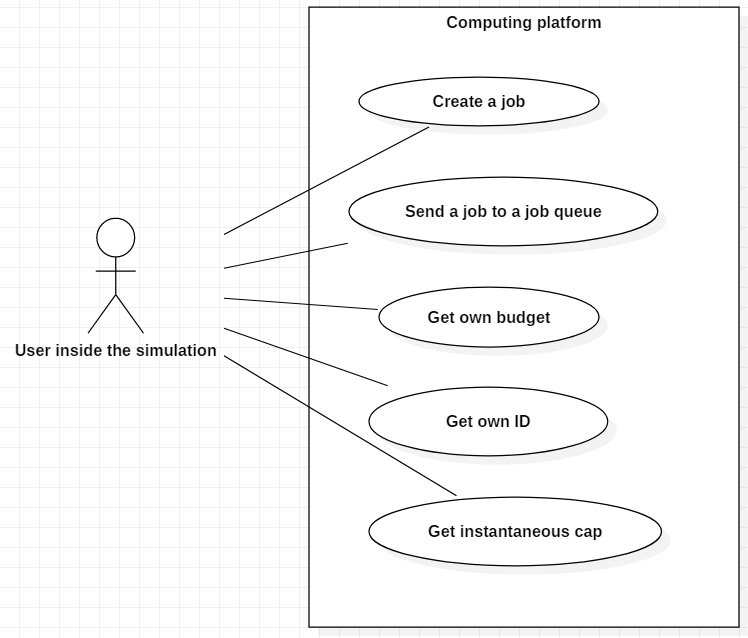
\includegraphics[width=0.95\textwidth]{UCD1.jpg}
\caption{\label{fig:image} Use case diagram of the users inside the simulation}
\end{figure}

\noindent
These users can be classified into three categories: IT staff members, who are the biggest users, researchers, who are the second biggest users, and students, who are the smallest users.
In the simulation, we have decided for our examples to make more students than researchers and more researchers than IT staff members, but this is a parameter that can be chosen by the users of the simulation. Each class of users has the same rights, it is only their parameters which may vary: the bigger users have a bigger budget and a bigger instantaneous cap. Actually only the students can be prevented from creating a job by their instantaneous cap. We have decided that their cumulative cap is represented by their lower budget, as the simulation only runs for a week.
\\ \\
In the use case diagram we can see that the users we simulate in our system can do various actions. We allow them access to their parameters but they cannot be changed by them for obvious security reasons. They can also access the computing system to create a job. They can finally send a job they created to a job queue of their choice. The job has a corresponding number of nodes it will be using, for a certain number of hours with a specific type of nodes. These parameters are decided directly by the simulated users when they create a job. The parameters will also result in a certain budget that will have to be spent by the users if they want to send the job to a queue, with each queue also having a different cost per hour.



\section{From outside the simulation}
Now we will explain how the users of our software can access and interact with our program, and what the software does in response. These users are the actual IT staff members who would be testing our simulation. We will begin by showing a rather broad view of the actions a user of our software can take and then explain some rather complicated actions more in detail, including how it works in the simulation.
\\ \\
We can see from the first diagram below that the user has a rather wide variety of actions possible. He can evaluate the scheduler, as this is a crucial feature of the simulator, because the scheduler is a capital factor of performance of the system. He can also change the scheduler. Indeed the program has been made so that the scheduler is a single class with a single function, so that the user of the simulation only has this unique function to change if he wants to use the simulation with another scheduler. That is why the evaluation of the scheduler is relevant even if we are using a rather inefficient first-in first-out scheduler here. 
\\ \\
Before the simulation starts, the user can of course choose the parameters that will be used inside of the simulation. This will be better explained on the diagram presented in fig. 2.3. Once the simulation has ended, the user can also access the results of the simulation, which correspond to many outputs that will be detailed in fig. 2.4. Finally, to verify that those results have a meaning, the user can check the tests of the simulation and make sure that all of them have passed, so that the code should be giving appropriate results.
\clearpage

\begin{figure}[!htbp]
\centering
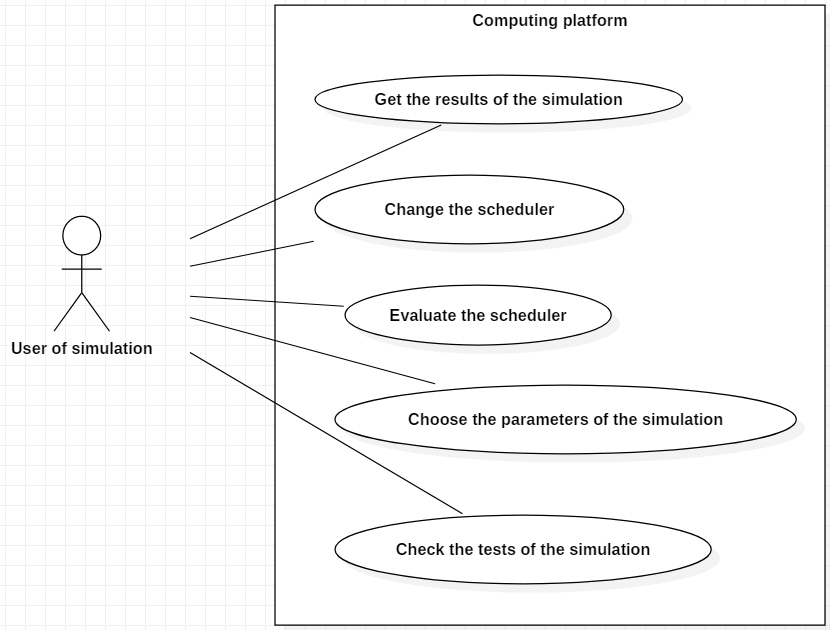
\includegraphics[width=\textwidth]{UCD2.jpg}
\caption{\label{fig:image} General use case diagram of the users of the simulation}
\end{figure}

\begin{figure}[!htbp]
\centering
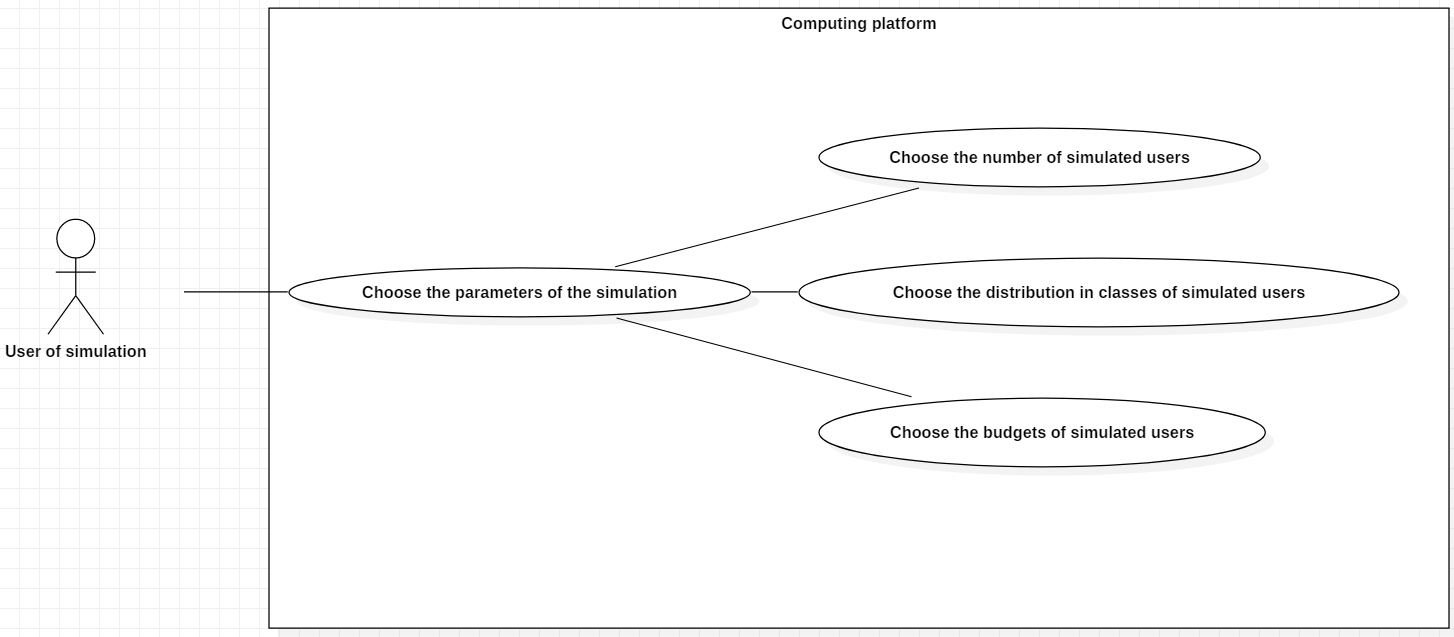
\includegraphics[width=1.2\textwidth]{UCD4.jpg}
\caption{\label{fig:image} Use case diagram of the users of the simulation detailing their choice of parameters for the simulation}
\end{figure}

\clearpage
\noindent
When he starts the simulation, the user has to select parameters. He has to choose the set of simulated users that will be observed. In order to generate this set of simulated users, he can choose the number of simulated users from each class: the number of IT staff members, the number of researchers and the number of students. For each of these simulated users, he also needs to choose a budget. In order to make the generation of a bigger amount of users less tedious and more random than with a single input file, we have added the possibility for the user not to choose the budget of each user generated. Indeed the user can also choose to keep the default values for the budgets of each class. We have put a fixed budget for the IT staff members and the students, but have added a random variable to the budget of the researchers to represent the fact that they can have additional budget granted to them. This way we can also test more functionalities without the need of an input. \\ \\

\begin{figure}[!htbp]
\centering
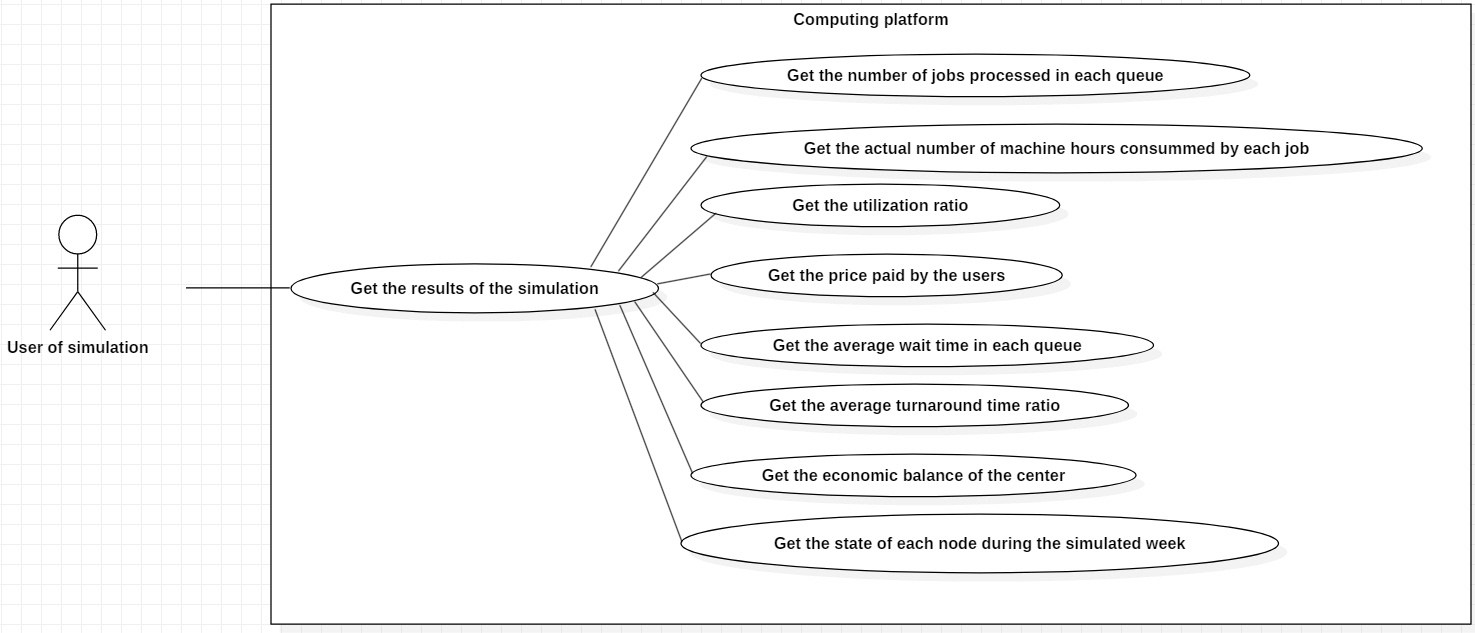
\includegraphics[width=1.2\textwidth]{UCD3.jpg}
\caption{\label{fig:image} Use case diagram of the users of the simulation detailing the outputs they can get from the simulation}
\end{figure}

\\
\noindent
Additionaly, the user of the simulation can view the results of the simulation in details. More precisely he can obtain the number of jobs processed in each of the three queues, get the actual number of machine hours that each job consummed, get the utilisation ratio, as well as the prices paid by the users, their average wait time for each of the four job queues, the average turnaround time ratio, the economic balance of the whole center, and finally we have added the possibility to view the state of each node during the simulated week. 
\\ \\
In order to show this, we have chosen to represent each of the three types of nodes: traditional, accelerated and specialized, by a matrix. We have recuperated the matrix class we use as well as a vector class used by this matrix class from an exercise of the course of C++. For our representation, For our representation, we have chosen the lines of the matrices to represent each a time step of one hour during the week. As there are 168 hours in a week, this is the number of rows our three matrices possess. The number of columns of our matrices is the number of nodes chosen for each type. In total there are always at least 128 nodes, which we have respected in our simulation where we chose by default 64 traditional nodes, 32 accelerated nodes and 32 specialized nodes, which makes it 128 nodes in total.
\\ \\

\begin{figure}[!htbp]
\centering
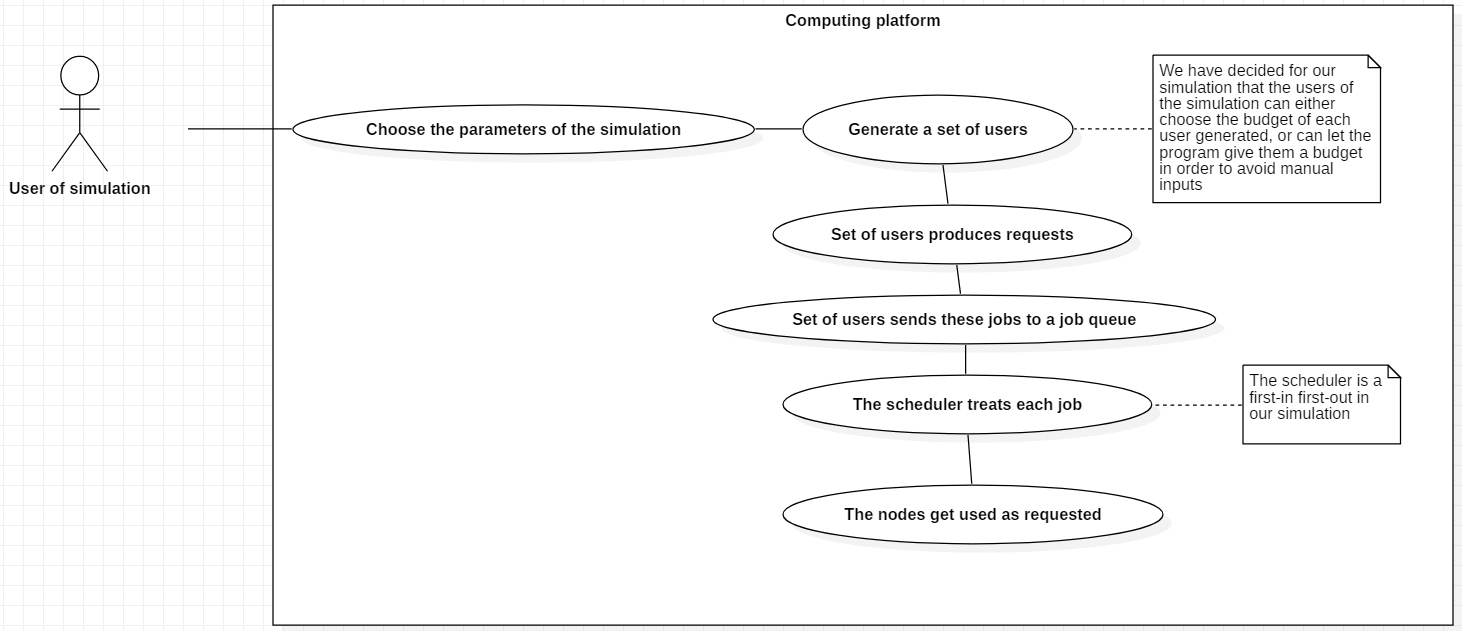
\includegraphics[width=1.2\textwidth]{UCD5.jpg}
\caption{\label{fig:image} Use case diagram of the users of the simulation detailing the process in the simulation}
\end{figure}
\\

\noindent
When the user of the simulator chooses the parameters, it is to generate a set of users. These simulated users produce requests during the simulated week. Each user has a probability of sending a job to a job queue depending on an exponential distribution. The size of the job, so the number of nodes used, also depends on an exponential distribution. The bigger users have a bigger chance of sending a request, so that at the end of the week, on average, they will have sent more requests. We used the exponential distribution so that the jobs would have more chance to be sent at a short interval, and so that bigger jobs happen more often than the smaller ones. We determine the duration of the job depending on the queue it is sent to, with a random variable so that not every job of a same queue has the same duration.
\\ \\
Once the simulated users have sent their requests to a chosen job queue, the scheduler takes each job and associates it with the necessary resources: the nodes, of the type requested. The nodes are used as soon as possible from the time the scheduler gets the request. For this simulation, since we are counting the time in hours, we do not simulate any delay of the scheduler or in the taking of the nodes. The scheduler directly links the job to the right resources, which means that the corresponding nodes are then used appropriately.
\\ \\
\clearpage
For this simulation we have chosen to consider the use of the software by the actual IT staff members who will use it, and inside of the simulation by the generated users. The actual users start the simulation with a set of parameters, and in this simulation the generated users send requests that are treated thanks to the scheduler linking the right job to the right nodes.




\chapter{Software requirements}
% appropriate models to represent the requirements (functional and non-functional); it is suggested to create a structured model, a behavioural model and a data flow model to capture the requirements of the simulation system.

\section{Functional model of the requirements}
\subsection{UML class diagram}
We have chosen to represent the requirements with a UML class diagram, which is a structured model, because we find it useful to code in a language like C++ that can be considered object oriented. It is also a good way to present the code with the different classes, their attributes and their methods and functions. It also shows how each class interacts with the others.
\\ \\
First we will see each class to present it, before showing how they are part of the software as a whole.

\\ \\

\begin{figure}[!htbp]
\centering
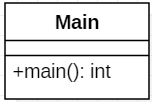
\includegraphics[width=0.2\textwidth]{Main.jpg}
\caption{\label{fig:image} Class diagram of Main}
\end{figure}
\\

\noindent
The Main class is what launches the simulator. It also starts the tests and the evaluation of the scheduler if that is necessary.


\\ \\

\begin{figure}[!htbp]
\centering
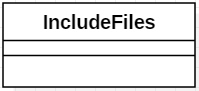
\includegraphics[width=0.3\textwidth]{IncludeFiles.jpg}
\caption{\label{fig:image} Class diagram of InclideFiles}
\end{figure}
\\

\noindent
The IncludeFiles class is a way to keep the dependencies used by every other class in a single file. It could also contain a function or a variable needed by most classes if it becomes needed.

\clearpage

\begin{figure}[!htbp]
\centering
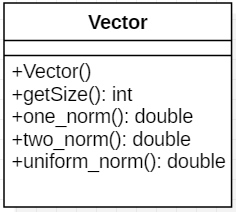
\includegraphics[width=0.3\textwidth]{Vector.jpg}
\caption{\label{fig:image} Class diagram of Vector}
\end{figure}

\begin{figure}[!htbp]
\centering
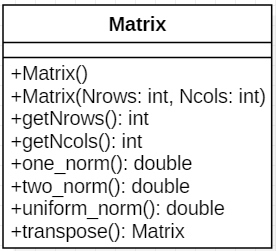
\includegraphics[width=0.3\textwidth]{Matrix.jpg}
\caption{\label{fig:image} Class diagram of Matrix}
\end{figure}
\\

\noindent
The Matrix class is used to represent the nodes as was previously explained. Itself, it uses the vector class. These classes were both taken from an exercise of the course of C++. There is one matrix for each type of node, which means one for the traditional, one for the accelerated and one for the specialized nodes.


\\ \\

\begin{figure}[!htbp]
\centering
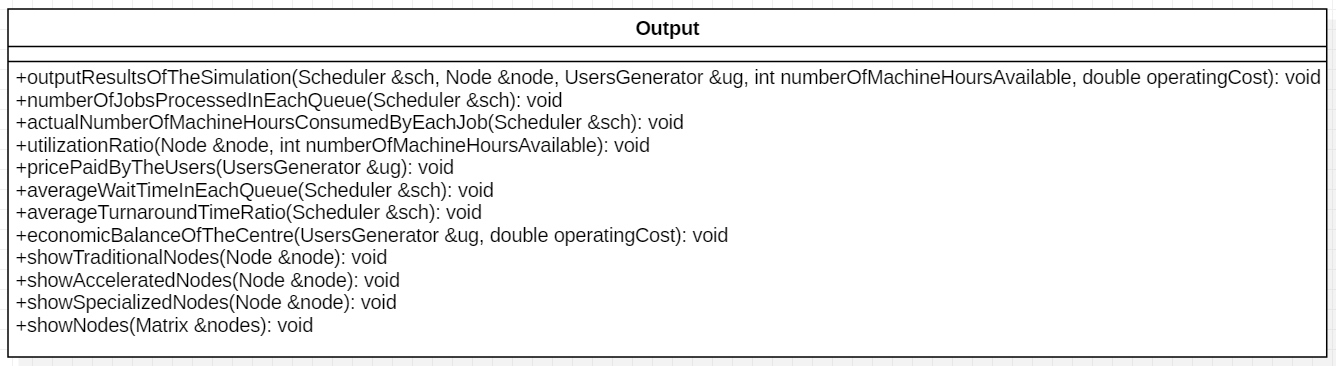
\includegraphics[width=1.3\textwidth]{Output.jpg}
\caption{\label{fig:image} Class diagram of Output}
\end{figure}
\\

\noindent
The Output class is used by the Main class in order to show the results of the simulation to the actual user as we have described in the first chapter, in fig. 2.4. The user sees these results at the end of the simulation.


\clearpage

\begin{figure}[!htbp]
\centering
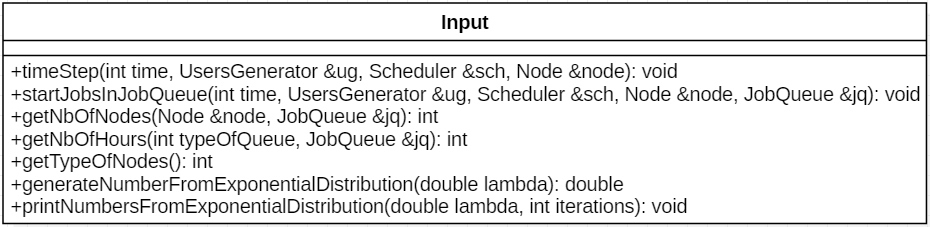
\includegraphics[width=1.3\textwidth]{Input.jpg}
\caption{\label{fig:image} Class diagram of Input}
\end{figure}
\\

\noindent
The Input class is used by the Main class to make the simulation progress in time. Its function timeStep makes everything needed for the time to go forward one hour. Indeed it chooses which simulated user sends which job request, what kind of job request and to which job queue. To do this, it uses its other functions.

\\ \\

\begin{figure}[!htbp]
\centering
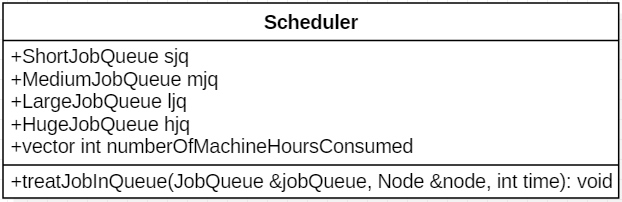
\includegraphics[width=\textwidth]{Sch.jpg}
\caption{\label{fig:image} Class diagram of Scheduler}
\end{figure}
\\

\noindent
The Scheduler class is used to link the jobs with the proper resources. When jobs are sent to a job queue by a user, it is the scheduler that decides which job is treated first and sends it to be taken care of by the right resources. Here, to have a simpler simulation, we have a first-in first-out scheduler.

\\ \\

\begin{figure}[!htbp]
\centering
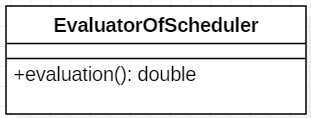
\includegraphics[width=0.6\textwidth]{EvalOfSch.jpg}
\caption{\label{fig:image} Class diagram of EvaluatorOfScheduler}
\end{figure}
\\

\noindent
The EvaluatorOfScheduler class evaluates the scheduler we have chosen for our implementation of the software. It tells us how long the scheduler treats a standard problem. To get a better approximation, this problem is repeated 1000 times and the result of the duration of the treatment is divided accordingly.

\clearpage

\begin{figure}[!htbp]
\centering
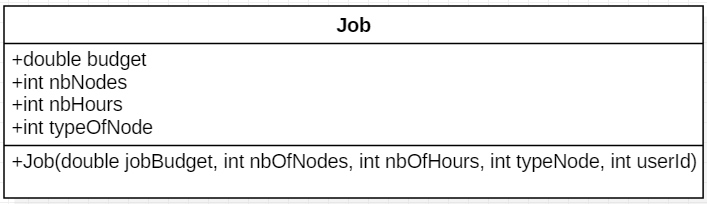
\includegraphics[width=1.2\textwidth]{Job.jpg}
\caption{\label{fig:image} Class diagram of Job}
\end{figure}
\\

\noindent
The Job class represents the jobs that are created by the users. Its attributes give the information needed for the right resources to be taken in order to treat each job. A job can be created by any simulated user if they have enough budget.

\\ \\

\begin{figure}[!htbp]
\centering
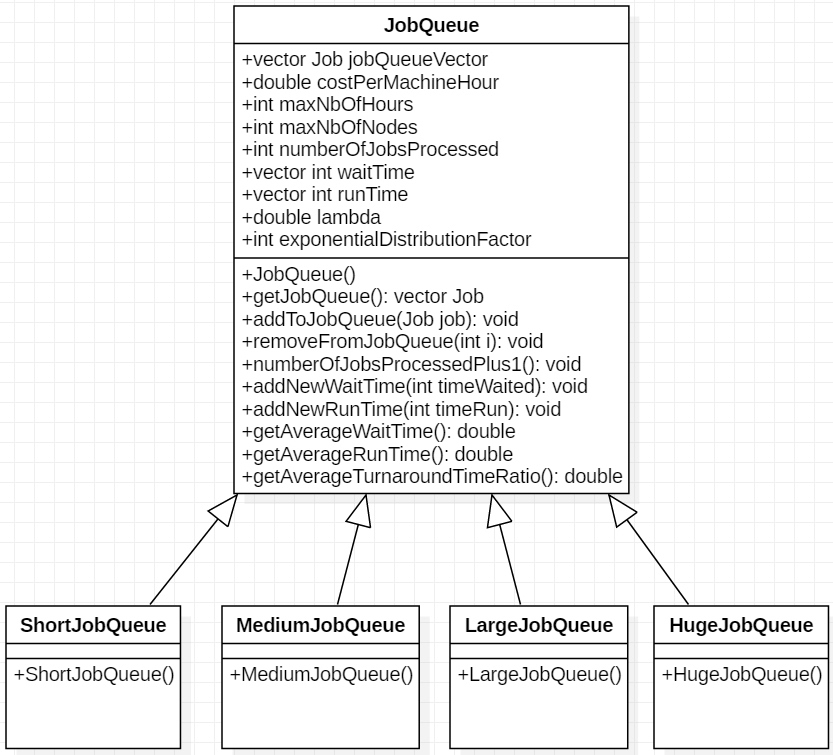
\includegraphics[width=\textwidth]{JobQueues.jpg}
\caption{\label{fig:image} Class diagram of the JobQueues}
\end{figure}
\\
\clearpage
\noindent
The JobQueue class is used by the scheduler to choose which job gets treated first. There are actually four job queues: a short one, a medium one, a large one and a huge one. Since they have all their attributes and functions in common, and are only different in the way these attributes are initialized, we have created a JobQueue class from which four classes, corresponding each to a specific job queue, inherits.

\\ \\

\begin{figure}[!htbp]
\centering
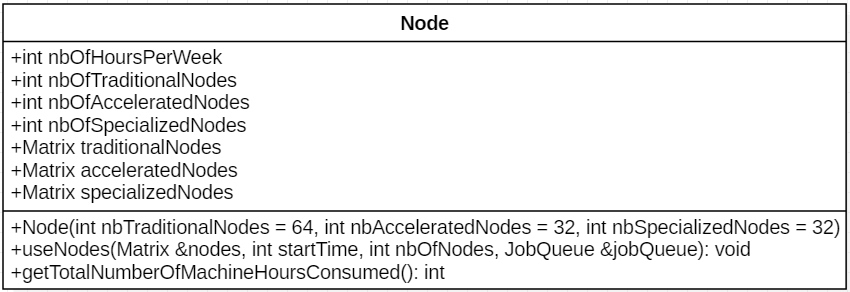
\includegraphics[width=1.2\textwidth]{Node.jpg}
\caption{\label{fig:image} Class diagram of Node}
\end{figure}
\\

\noindent
The Node class contains three matrices to represent the different nodes as we have previously explained. It represents the resources of the system. In each matrix, a value of zero means that the node has not been used, while a value of one means that the node has been used. It lets us see the advances of our simulation and how the resources are used, as well as what resources we can use at a certain point in time. The nodes treat the jobs. Indeed, at first, the nodes are all initialized to zero, but once a job is treated the corresponding nodes get the value of one.

\\ \\

\begin{figure}[!htbp]
\centering
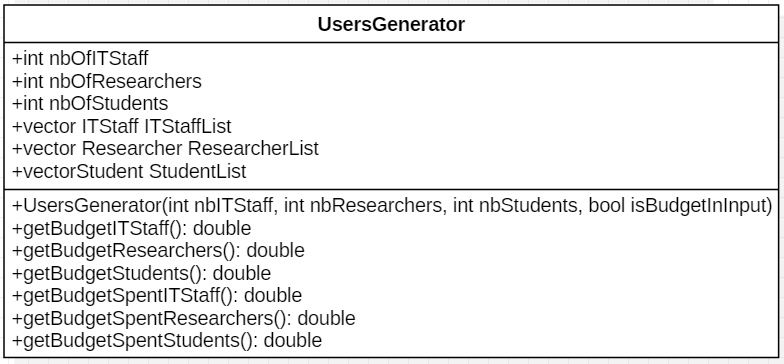
\includegraphics[width=1.2\textwidth]{UsersGenerator.jpg}
\caption{\label{fig:image} Class diagram of UsersGenerator}
\end{figure}
\\
\clearpage
\noindent
The UsersGenerator class lets us generate a set of users accordingly to the parameters chosen by the user of the simulation. To represent each set of users while respecting their classes, three vectors are created: a vector of ITStaff, a vector of Researcher and a vector of Student. Each vector contains the users generated of the corresponding class.

\\ \\

\begin{figure}[!htbp]
\centering
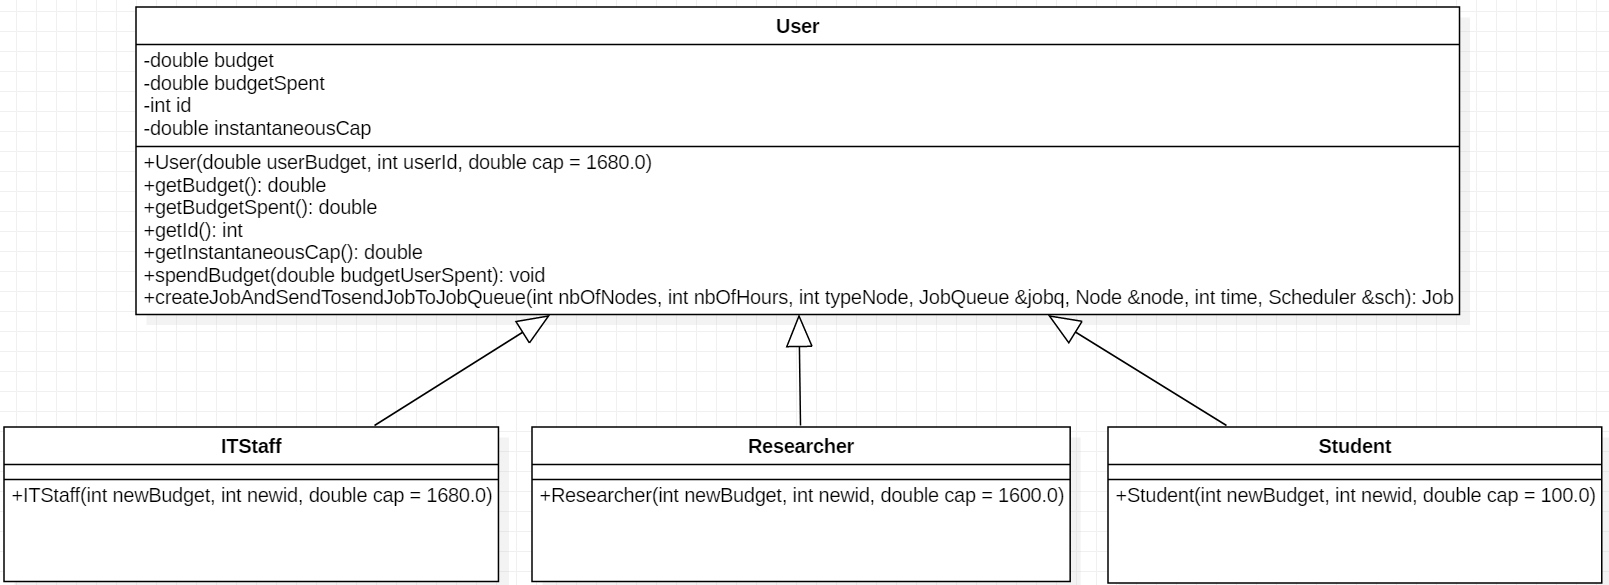
\includegraphics[width=1.3\textwidth]{Users.jpg}
\caption{\label{fig:image} Class diagram of the Users}
\end{figure}
\\

\noindent
The User class is the base class for the simulated users. The ITStaff, Researcher and Student classes all inherit from it. Like for the job queues, they all have the same attributes and functions but those attributes have different values. It is these classes that can generate jobs and send them to a queue of their own choice.

\clearpage

\begin{figure}[!htbp]
\centering
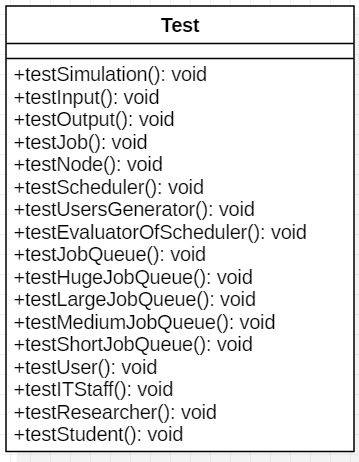
\includegraphics[width=0.7\textwidth]{Test.jpg}
\caption{\label{fig:image} Class diagram of Test}
\end{figure}
\\

\noindent
The Test class is used to test every other class. While there are tests inside of the other classes, it is this class that contains the unit testing. It has a function testSimulation that runs all of the tests. If this one passes it means that all of our tests pass. We coded each function with assert so that if a test fails, the program cannot finish running and we do not get false results unknowingly.

\clearpage

\begin{figure}[!htbp]
\centering
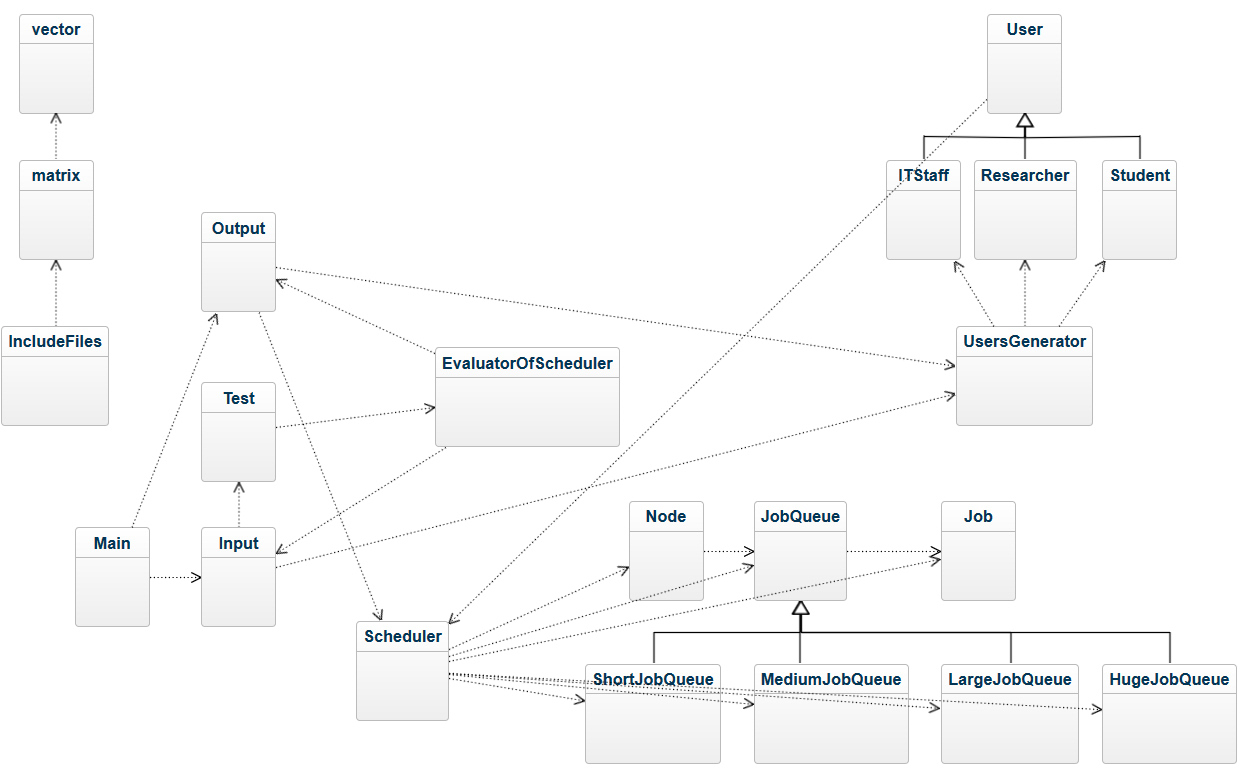
\includegraphics[width=1.3\textwidth]{umlDiagram.jpg}
\caption{\label{fig:image} Class diagram of the project}
\end{figure}
\\

\noindent
Every class depends on the IncludeFiles class but to make this diagram easier to read, we have not represented these dependencies. In this diagram we can see that the Main class uses only the Input and Output classes to have access to all the classes it actually needs. It also uses the Input to progress trough each time step and the Output to show the final results of the simulation. Of course it is also the Main class that runs the evaluation of the scheduler as well as the various tests of the other classes. The scheduler itself manages the link between the resources, so the nodes, and the job queues containing the jobs sent by the users. The users themselves exist because they are generated by UsersGenerator. Many of the links between classes are indirect, but it is indeed the users who create the jobs before sending them to the scheduler. 
\\ \\
In order to get proper results, during one run of the simulation, there is only one instance of the scheduler, so one instance of each queue used. There is also a single instance of the nodes represented by unique matrices. The UsersGenerator is also unique in order to keep the same users during the whole simulation.



\clearpage
\noindent

\subsection{Sequence diagram}
We will be presenting the sequence diagram of our simulation doing its main purpose: that of its users creating jobs and the jobs being treated. This is a behavioural model.

\\ \\

\begin{figure}[!htbp]
\centering
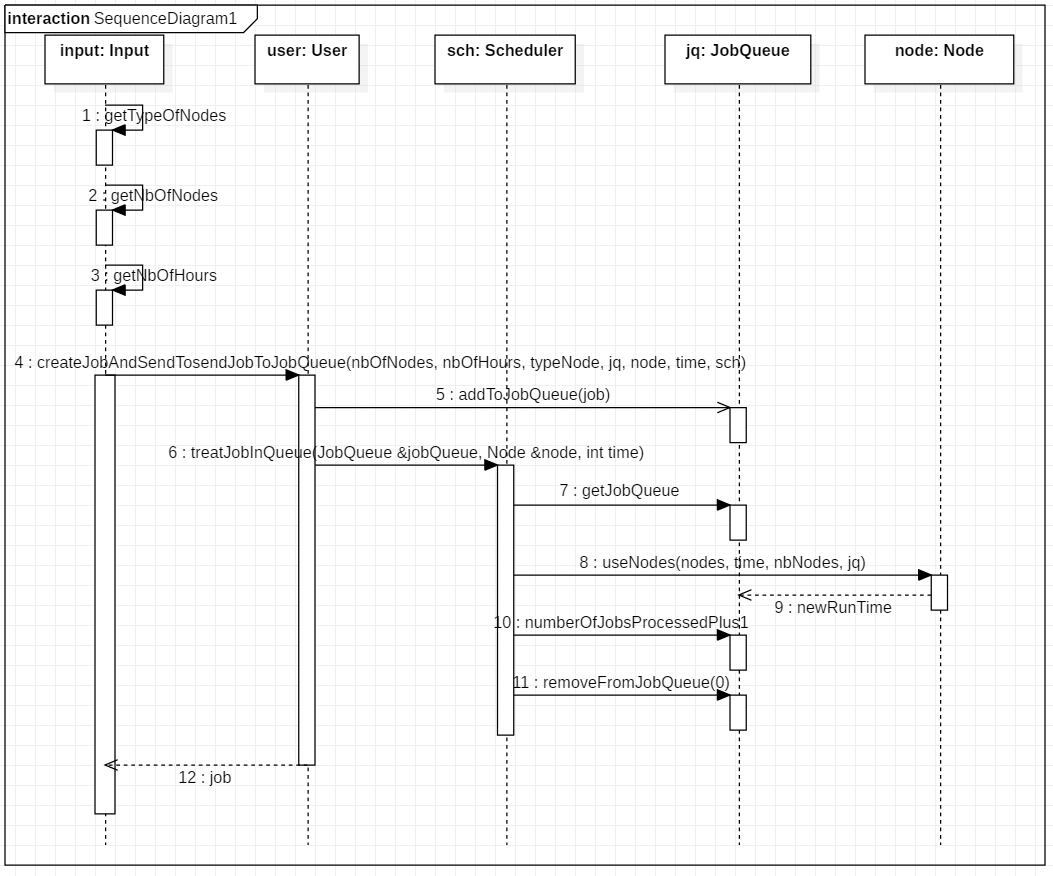
\includegraphics[width=1.3\textwidth]{SequenceDiag.jpg}
\caption{\label{fig:image} Sequence diagram of the treatment of a job at a certain time step}
\end{figure}
\\

\noindent
In this sequence diagram we can see that first the Input object chooses the type of nodes the job created will be requesting. It also chooses its number of nodes and the number of hours it will approximately take to execute. There is also a time corresponding to the current date in the week of the simulation, a job queue to which the job will be sent, and the scheduler and nodes used during the simulation to treat the jobs.
\\ \\
Then it sends a message to the user that will be sending the job request to the scheduler. First this user adds the job to the chosen job queue: it is one of the job queues instantiated in the scheduler, which can be a short job queue, a medium one, a large one or a huge one. If it is before Friday 5pm the job queue will be one of the first three, if it is after, the job queue will be the huge one, as it is the only queue active during the weekend and it is only active then.
\\ \\
Next the user will send its request to the scheduler. The scheduler will first retrieve the appropriate job queue. Here the job treated is always the job of index zero because it is a first-in first-out scheduler. This way, the scheduler will know that it has to send the information corresponding to this job to the nodes.
\\ \\
The appropriate nodes will then be used, which is represented by the modification of the matrix corresponding to the type of nodes requested: traditional nodes, accelerated nodes or specialized nodes. Once that is done, the run time can be sent to the job queue used. The number of jobs processed is increased by one and the job that has been treated is removed from the job queue.








\clearpage
\noindent

\section{Non-functional models of the requirements}
\subsection{Data flow diagram}
We will now be presenting a data flow diagram. This non functional model lets us see how the data is transfered and treated during the simulation.

\\ \\

\begin{figure}[!htbp]
\centering
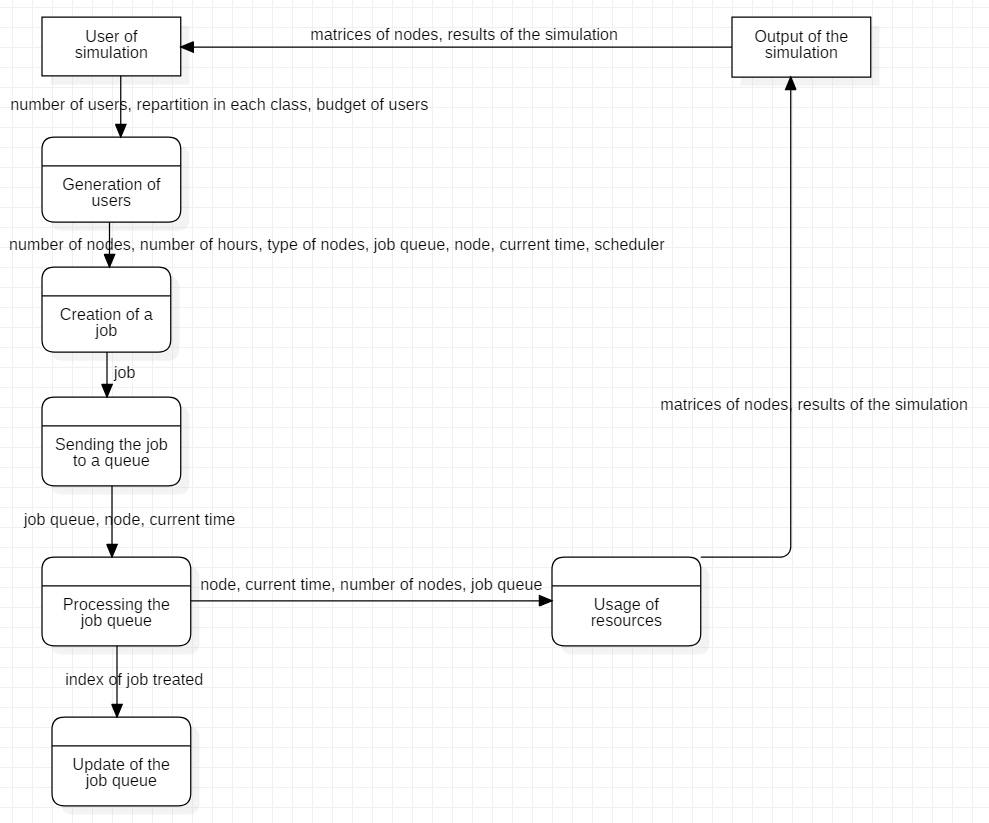
\includegraphics[width=1.3\textwidth]{DataFlowDiag.jpg}
\caption{\label{fig:image} Data flow diagram of the software}
\end{figure}
\\

\noindent
We can see that it is the users of the simulation who input the first data: they choose the parameters of the set of users. As we have previously explained, it is optional for the user to input the budget of each user, as the simulation can also do it for more convenience. With these parameters, the set of users gets generated. 
\\ \\
These users can then send data to create a job that will be treated with the available resources. The simulated users can therefore send the number of nodes the job will be taking, as well as its number of hours, the type of the nodes used, the job queue that the job will be sent to, the node and scheduler of the simulation, and finally the current time.
\\ \\
Once the job has been created, its instance can be sent to the job queue so that it can be processed. Once the job has been treated, its index is sent to the job queue so that it can be removed from it. Indeed, only the jobs waiting to be processed are in the job queue.
\\ \\
To treat this job, the right resources need to be used. That is why the node, the current time, the number of nodes used and the job queue chosen are sent to the nodes so that the matrices of nodes can be updated.
\\ \\
After all this processing is done for the whole week and for every user, the final matrices of nodes and the results of the simulation can be sent as an output back to the user of the simulation who sent the first parameters. More details of the results of the simulation can be seen in fig 3.5 of the Output class that contains every final output of the simulation. This way, the users of the simulation choose its parameters as the requirements ask, and receive the results of the simulated week with the users it generated and their job requests.








\chapter{Test plan}
% Explain what needs to be tested and how you will implement the tests. Ensure you have adequately considered both lower level unit and integration testing, and explain your choice of test inputs.

In order to do the testing of the simulation, we have chosen to do our tests on two different scales. First we do the test of the inputs inside of the functions, to check whether this input is coherent. Then we also have a Test class that contains the unit testing of every class of the software. The tests were all made with the assert() function so that the user of the simulation instantly knows if the software could produce wrong results. This way, the program can not accept wrong input or a wrong implementation.
First we will be presenting the tests inside of the functions, and then the unit tests of each class.


\section{Tests inside of the function}

In order to check the input of the functions, we often put one or more assert at the very beginning of the function to check if running it will give us appropriate results. We have put those assert in the following classes: Input, Job, JobQueue, Node, Output, Scheduler, User and UsersGenerator. Of course there are also many assert in the Test class, but we will see it in more details in the next section.


\begin{lstlisting}[caption=timeStep function of the class Input, label={lst:code1}, frame=single]
void Input::timeStep(int time, UsersGenerator &ug, Scheduler &sch,
Node &node) {
	// We check if the time is possible within the week
	assert(time >= 0 && time <= 168);

	// We randomly choose which user will submit a job at this time
	// and what job it will be
	if (time < 104) {
		...
	}
	else {
		...
	}
}
\end{lstlisting}
\clearpage
\noindent
\\ \\
As we can see we are checking if the time is possible within the time frame of the week. Indeed the time needs to be greater or equal to zero but lesser or equal to 168, which is the number of hours in the week. This test can be seen in every function with time as a parameter for the same reasons, so we will not be explaining it again. The following listings show the other instances of this test.



\begin{lstlisting}[caption=startJobsInJobQueue function of the class Input, label={lst:code1}, frame=single]
void Input::startJobsInJobQueue(int time, UsersGenerator &ug, Scheduler &sch,
Node &node, JobQueue &jq) {
	// We check if the time is possible within the week
	assert(time >= 0 && time <= 168);
	...
}
\end{lstlisting}

\begin{lstlisting}[caption=treatJobInQueue function of the class Scheduler, label={lst:code1}, frame=single]
void Scheduler::treatJobInQueue(JobQueue &jobQueue, Node &node, int time) {
	// We check if the time is possible within the week
	assert(time >= 0 && time <= 168);
	...
}
\end{lstlisting}

\begin{lstlisting}[caption=createJobAndSendTosendJobToJobQueue function of the class User, label={lst:code1}, frame=single]
Job User::createJobAndSendTosendJobToJobQueue(int nbOfNodes, int nbOfHours, 
int typeNode, JobQueue &jobq, Node &node, int time, Scheduler &sch) {
	assert(time >= 0 && time <= 168);
	...
}
\end{lstlisting}

\begin{lstlisting}[caption=useNodes function of the class Node, label={lst:code1}, frame=single]
void Node::useNodes(Matrix &nodes, int startTime, int nbOfNodes, JobQueue &jobQueue) {
	assert(startTime >= 0 && startTime <= nbOfHoursPerWeek);
	...
}
\end{lstlisting}


\noindent
\\ \\
We also have tests on other input than the current time of the simulation. Indeed when the type of node is needed, it is also verified. We have chosen that the type of node used is represented by an integer that can be zero, one or two, as there are three types of node. Therefore, when a parameter is the type of node, we check that it is one of the possible values.

\begin{lstlisting}[caption=Job constructor of the class Job, label={lst:code1}, frame=single]
Job::Job(double jobBudget, int nbOfNodes, int nbOfHours, int typeNode, 
int userId) {
    ...
	assert(typeNode >= 0 && typeNode <= 2);
	...
}
\end{lstlisting}

\noindent
\\ \\
For the next functions there are also tests that do not use assert, as an error there does not means that the software does not work. Indeed, at the beginning we do use some assert to check the input. However, we also check if the job can be created by the user who is trying to create and send his request. 
\\ \\
\noindent
For this, we first check if the instantaneous cap of the user is sufficient. If so, we can proceed, otherwise we print a message and return an empty job object.
\\ \\
If the cap was big enough, we check the budget of the user. We do it the same way as previously, by printing an error message and returning an empty job if the creation of the job cannot be done by the user.
\\ \\
Finally we check if the job request will not take more time than the maxiumum time of the job queue the user has chosen, and we also check if  the number of nodes is not too great for the chosen queue. If one of these conditions is not respected, an appropriate error message is printed and an empty job is returned. Otherwise, all the tests have been passed and the job can be sent to the queue, after which the scheduler can affect the right resources to it.


\begin{lstlisting}[caption=createJobAndSendTosendJobToJobQueue function of the class User, label={lst:code1}, frame=single]
Job User::createJobAndSendTosendJobToJobQueue(int nbOfNodes, int nbOfHours, 
int typeNode, JobQueue &jobq, Node &node, int time, Scheduler &sch) {
	...
	assert(typeNode >= 0 && typeNode <= 2);

	double jobBudget = jobq.costPerMachineHour * nbOfHours;
	if (jobBudget > getInstantaneousCap()) {
		cout << "Instantaneous cap too low to create this job!" 
		<< " Budget needed: " << jobBudget << " Cap: " 
		<< getInstantaneousCap() << "\n";
		return Job(NULL, NULL, NULL, NULL, NULL);
	}

	Job job = Job(jobBudget, nbOfNodes, nbOfHours, typeNode, getId());
	// Check wether the user has enough budget to create the job
	if (jobBudget > getBudget()) {
		cout << "Not enough budget to create this job!" 
		<< " Budget needed: " << jobBudget 
		<< " Budget possessed: " << getBudget() << "\n";
		return Job(NULL, NULL, NULL, NULL, NULL);
	}
	
	if (job.nbHours <= jobq.maxNbOfHours && 
	job.nbNodes <= jobq.maxNbOfNodes) {
		...
		sch.treatJobInQueue(jobq, node, time);
	}
	else if (job.nbHours > jobq.maxNbOfHours) {
		cout << "The number of hours is too high for this queue!\n";
		return Job(NULL, NULL, NULL, NULL, NULL);
	}
	else {
		cout << "The number of nodes is too high for this queue!\n";
		return Job(NULL, NULL, NULL, NULL, NULL);
	}

	sch.numberOfMachineHoursConsumed.push_back(nbOfHours);

	return Job(jobBudget, nbOfNodes, nbOfHours, typeNode, getId());
}
\end{lstlisting}


\noindent
\\ 
To come back to the tests made of assert, the Input class has more of those. First it has a function that needs to know the type of job queue to know what order of job duration it should generate. Since there are four types of queue: short, medium, large and huge, we decided to represent the type of queue by an integer between zero and three. We check if the parameter input corresponds to this with the assert at the very beginning of the function.

\\ \\

\begin{lstlisting}[caption=getNbOfHours function of the class Input, label={lst:code1}, frame=single]
int Input::getNbOfHours(int typeOfQueue, JobQueue &jq) {
	assert(typeOfQueue >= 0 && typeOfQueue <= 3);

	// We decide that the users will use each queue appropriately
	int nbHours;
	...
	return nbHours;
}
\end{lstlisting}

\noindent
\\ \\
The Input class is also responsible for the exponential distribution representation. It has a function that returns a number generated with this distribution with a parameter lambda. In order to check the validity of this function we also have a function that prints many results from the exponential distribution. However we had to check these results by exporting them as plotting seemed  bit complicated to do directly in C++. In both of these functions, lambda has to be positive, as it is in the definition of the exponential distribution. Besides, in the printing function, the quantity of numbers shown is asked, which of course also has to be positive. In the program, we chose the value of lambda empirically when seeing the use of the machine by each class of the users.



\begin{lstlisting}[caption=generateNumberFromExponentialDistribution function of the class Input, label={lst:code1}, frame=single]
double Input::generateNumberFromExponentialDistribution(double lambda) {
	assert(lambda > 0);

	random_device rd;
	mt19937 generator(rd());
	exponential_distribution <double> distribution(lambda);
	double res = distribution(generator);

	return res;
}
\end{lstlisting}


\begin{lstlisting}[caption=printNumbersFromExponentialDistribution function of the class Input, label={lst:code1}, frame=single]
void Input::printNumbersFromExponentialDistribution(double lambda,
int iterations) {
	assert(lambda > 0);
	assert(iterations > 0);

	for (int i = 0;i < iterations;i++) {
		cout << generateNumberFromExponentialDistribution(lambda) 
		<< "\n";
	}
}
\end{lstlisting}


\noindent
\\ \\
Besides what we have already shown, the Job class constructor also has assert for its other parameters. Indeed, the given job budget has to be positive, as well as the number of nodes used and the number of hours. We have chosen to offer the possibility to make these values equal to zero in case someone wants to make an empty job. As we have previously explained, the type of nodes is between zero and two. Finally, we have chosen that the user ID are all greater than or equal to zero and this is the way we generate our users.

\\ \\

\begin{lstlisting}[caption=Job function of the class Job, label={lst:code1}, frame=single]
Job::Job(double jobBudget, int nbOfNodes, int nbOfHours, int typeNode, int userId) {
	assert(jobBudget >= 0);
	assert(nbOfNodes >= 0);
	assert(nbOfHours >= 0);
	assert(typeNode >= 0 && typeNode <= 2);
	assert(userId >= 0);
	...
}
\end{lstlisting}


\noindent
\\ \\
The removeFromJobQueue function removes a job of a given index from the job queue. For the index to be possible, it has to be between zero and the maximum index of the job queue, which is the size of this job queue minus one here.


\begin{lstlisting}[caption=removeFromJobQueue function of the class JobQueue, label={lst:code1}, frame=single]
void JobQueue::removeFromJobQueue(int i) {
	// We check that i is a possible index of the job queue vector
	assert(i >= 0);
	assert(i < jobQueueVector.size());

	jobQueueVector.erase(jobQueueVector.begin() + i);
}
\end{lstlisting}


\noindent
\\ \\
The next function adds a wait time to a list that is used in Output to calculate the average wait time. Since it is a time, it needs to be greater than or equal to zero.


\begin{lstlisting}[caption=addNewWaitTime function of the class JobQueue, label={lst:code1}, frame=single]
void JobQueue::addNewWaitTime(int timeWaited) {
	assert(timeWaited >= 0);

	waitTime.push_back(timeWaited);
}
\end{lstlisting}

\noindent
\\ \\
The addNewRunTime function works the exact same way, for a run time instead of a wait time. Because of this we check here that the run time added is greater than or equal to zero


\begin{lstlisting}[caption=addNewRunTime function of the class JobQueue, label={lst:code1}, frame=single]
void JobQueue::addNewRunTime(int timeRun) {
	assert(timeRun >= 0);

	runTime.push_back(timeRun);
}
\end{lstlisting}


\noindent
\clearpage
For useNodes, we have a number of nodes to use. This number of nodes has to be greater than or equal to zero


\begin{lstlisting}[caption=useNodes function of the class Node, label={lst:code1}, frame=single]
void Node::useNodes(Matrix &nodes, int startTime, int nbOfNodes, 
JobQueue &jobQueue) {
	assert(startTime >= 0 && startTime <= nbOfHoursPerWeek);
	assert(nbOfNodes >= 0);
	...
}
\end{lstlisting}


\noindent
\\ \\
The node constructor checks every input the same way as the job contructor did. Indeed the number of each type of node has to be greater than or equal to zero. Additionally the total number of nodes has to be at greater than or equal to 128. In our simulation we have chosen a default value of 128 for the total number of nodes, with 64 traditional nodes, 32 accelerated nodes and 32 specialized nodes, as we decided that for most jobs the traditional nodes may be sufficient but some really big jobs can require the two other types of nodes.


\begin{lstlisting}[caption=Node constructor of the class Node, label={lst:code1}, frame=single]
Node::Node(int nbTraditionalNodes, int nbAcceleratedNodes, 
int nbSpecializedNodes) {
	assert(nbTraditionalNodes >= 0);
	assert(nbAcceleratedNodes >= 0);
	assert(nbSpecializedNodes >= 0);
	assert(nbTraditionalNodes + nbAcceleratedNodes + nbSpecializedNodes 
	>= 128);
	...
}
\end{lstlisting}

\noindent
\\ \\
The user constructor checks every input the same way as the node and job contructors did. The instantaneous cap and user budget have to be strictly greater than zero because a user that cannot spend budget or create job requests makes no sense in our simulation. Besides, the user ID is greater than or equal to zero.


\begin{lstlisting}[caption=User constructor of the class User, label={lst:code1}, frame=single]
User::User(double userBudget, int userId, double cap) {
	assert(userBudget > 0);
	assert(userId >= 0);
	assert(cap > 0);

	budget = userBudget;
	id = userId;
	budgetSpent = 0;
	instantaneousCap = cap;
}
\end{lstlisting}

\noindent
\clearpage
For the spendBudget function, we need to make sure that the budget we spend is greater than or equal to zero.


\begin{lstlisting}[caption=spendBudget function of the class User, label={lst:code1}, frame=single]
void User::spendBudget(double budgetUserSpent) {
	assert(budgetUserSpent >= 0);

	budget = budget - budgetUserSpent;
	budgetSpent += budgetUserSpent;
}
\end{lstlisting}


\noindent
\\ \\
For the UsersGenerator constructor, we need to check that the number of the users of each class is greater than or equal to zero. These numbers correspond to the parameters of the simulator given by the users of the simulation.


\begin{lstlisting}[caption=UsersGenerator constructor of the class UsersGenerator, label={lst:code1}, frame=single]
UsersGenerator::UsersGenerator(int nbITStaff, int nbResearchers, 
int nbStudents, bool isBudgetInInput) {
	assert(nbITStaff >= 0);
	assert(nbResearchers >= 0);
	assert(nbStudents >= 0);
	...
}
\end{lstlisting}


\noindent
\\ \\
For the treatJobInQueue function, we have to make sure that the job queue does contain at least one job that can be treated. We also check that the type of node given as parameter to the job corresponds to the existing types of nodes, which means it is between zero and two.


\begin{lstlisting}[caption=treatJobInQueue function of the class Scheduler, label={lst:code1}, frame=single]
void Scheduler::treatJobInQueue(JobQueue &jobQueue, Node &node, int time) {
	// We check if the time is possible within the week
	assert(time >= 0 && time <= 168);
	assert(jobQueue.getJobQueue().size() > 0);

	Job job = jobQueue.getJobQueue()[0];
	int nodeType = job.typeOfNode;
	assert(nodeType >= 0 && nodeType <= 2);
	...
}
\end{lstlisting}

\noindent
\\ \\
For the utilizationRatio function, the number of machine hours available during the week is given as a parameter. Since the simulation would make no sense if this number was null, we ask for the number to be strictly greater than zero. Besides, it prevents possible problems from the division by this number, so that we can avoid any division by zero.

\clearpage
\begin{lstlisting}[caption=utilizationRatio function of the class Output, label={lst:code1}, frame=single]
void Output::utilizationRatio(Node &node, int numberOfMachineHoursAvailable) {
	assert(numberOfMachineHoursAvailable > 0);

	cout << "Utilization ratio of the machine: " <<
	((double)(node.getTotalNumberOfMachineHoursConsumed()))/
	((double)numberOfMachineHoursAvailable) << "\n";

	cout << "\n";
}
\end{lstlisting}


\noindent
\\ \\
For the economicBalanceOfTheCentre function, we ask an operating cost. This cost has to be greater than or equal to zero. We have chosen the value of the operating cost so that the economic balance is null if the machine is used half as much as it can be used.


\begin{lstlisting}[caption=economicBalanceOfTheCentre function of the class Output, label={lst:code1}, frame=single]
void Output::economicBalanceOfTheCentre(UsersGenerator &ug, 
double operatingCost) {
	assert(operatingCost >= 0);
	...
}
\end{lstlisting}




\noindent
\\ \\
However since we are coding in C++, not all inputs can be tested. Indeed the type of each input cannot be verified. Still, we check that the values of the input make sense. Moreover, We add to those tests of input the tests of the functions of each class, and of the classes themselves. This is how unit testing is part of our test plan.











\clearpage
\section{Unit tests in the Test class}

Inside of the test class, we do unit testing for every class used in the simulation. In order to keep this clear, we do one function that tests one class. There is a function that is called in the main that itself calls all the functions of the Test class to show the tests for the whole simulation. This way, if the code gets broken, it will be visible as soon as the simulation tries the tests and fails, and we can see whether the output values are meaningful. We will be presenting here the test functions. For the Output class, no detailed tests could be done, so a simple instantiating of it was made. Here is the corresponding function:

\begin{lstlisting}[caption=testOutput function of the class Test, label={lst:code1}, frame=single]
void Test::testOutput() {
	Output out;
}
\end{lstlisting}



\noindent
\\ \\
There are classes where we could not use assert to test them so we instantiated them and started their functions to check whether they seemed to work normally:

\begin{lstlisting}[caption=testEvaluatorOfScheduler function of the class Test, label={lst:code1}, frame=single]
void Test::testEvaluatorOfScheduler() {
	EvaluatorOfScheduler eval;
	eval.evaluation();
}
\end{lstlisting}

\begin{lstlisting}[caption=testInput function of the class Test, label={lst:code1}, frame=single]
void Test::testInput() {
	Input in;
	UsersGenerator ug = UsersGenerator(5, 30, 500, false);
	Scheduler sch;
	Node node;
	in.timeStep(7, ug, sch, node);
}
\end{lstlisting}

\begin{lstlisting}[caption=testScheduler function of the class Test, label={lst:code1}, frame=single]
void Test::testScheduler() {
	Scheduler sch;
	Node node;
	Job job(60, 36, 2, 0, 36);
	sch.mjq.addToJobQueue(job);
	sch.treatJobInQueue(sch.mjq, node, 16);

}
\end{lstlisting}

\noindent
\\ \\ 
For the other classes we were better able to test how they reacted to our calls and if the results they gave us was what was expected from the data we gave them as parameters.

\clearpage
\begin{lstlisting}[caption=testJob function of the class Test, label={lst:code1}, frame=single]
void Test::testJob() {
	Job job = Job(60, 10, 2, 1, 3);

	assert(job.budget == 60);
	assert(job.nbNodes == 10);
	assert(job.nbHours == 2);
	assert(job.typeOfNode == 1);
\end{lstlisting}

\noindent
\\ \\ 
We instantiate a job object with a set of parameters. We check that the resulting object has the correct attributes.


\begin{lstlisting}[caption=testNode function of the class Test, label={lst:code1}, frame=single]
void Test::testNode() {
	Node node;
	Node node2(64, 128, 64);

	assert(node.nbOfTraditionalNodes == 64 && node.nbOfAcceleratedNodes 
	== 32 && node.nbOfSpecializedNodes == 32);
	assert(node2.nbOfTraditionalNodes == 64 && node2.nbOfAcceleratedNodes 
	== 128 && node2.nbOfSpecializedNodes == 64);
	assert(node.nbOfHoursPerWeek == 168);
	assert(node.traditionalNodes.getNrows() == node.nbOfHoursPerWeek 
	&& node.traditionalNodes.getNcols() == node.nbOfTraditionalNodes);
	assert(node.acceleratedNodes.getNrows() == node.nbOfHoursPerWeek 
	&& node.acceleratedNodes.getNcols() == node.nbOfAcceleratedNodes);
	assert(node.specializedNodes.getNrows() == node.nbOfHoursPerWeek 
	&& node.specializedNodes.getNcols() == node.nbOfSpecializedNodes);

	MediumJobQueue mjq;
	node.useNodes(node.traditionalNodes, 15, 200, mjq);
	
	Matrix resultTradiNodes = Matrix(node.nbOfHoursPerWeek, 
	node.nbOfTraditionalNodes);
	for (int i = 15;i < 18;i++) {
		for (int j = 0;j < resultTradiNodes.getNcols();j++)
			resultTradiNodes[i][j] = 1;
	}

	for (int j = 0;j < 8;j++)
		resultTradiNodes[18][j] = 1;

	assert(node.traditionalNodes == resultTradiNodes);
	assert(mjq.getAverageWaitTime() == 0);
	assert(mjq.getAverageRunTime() == 3);

	assert(node.getTotalNumberOfMachineHoursConsumed() == 4);
}
\end{lstlisting}

\noindent
\\ \\ 
We instantiate two node objects, one with a given set of parameters and the other with default values. We check that the resulting objects both have the correct attributes. We check that the sizes of the resulting matrices of nodes have the right dimensions. We then try to use some traditional nodes and check that the result is as expected by producing the expected matrix result and comparing it to the one we obtain by using the function useNodes. Finally we check that the average wait time, average run time and total number of machine hours consummed have the value they should.

\clearpage
\begin{lstlisting}[caption=testUsersGenerator function of the class Test, label={lst:code1}, frame=single]
void Test::testUsersGenerator() {
	UsersGenerator ugRandomBudget(2, 10, 20, false);
	UsersGenerator ugChosenBudget(0, 0, 0, true);

	for (int i = 0;i < ugRandomBudget.ITStaffList.size();i++)
		assert(ugRandomBudget.ITStaffList[i].getBudget() == 1680.0);
	
	for (int i = 0;i < ugRandomBudget.ITStaffList.size();i++)
		assert(ugRandomBudget.ResearcherList[i].getBudget() >= 800.0 
		&& ugRandomBudget.ResearcherList[i].getBudget() <=1600.0);

	for (int i = 0;i < ugRandomBudget.ITStaffList.size();i++)
		assert(ugRandomBudget.StudentList[i].getBudget() == 480.0);

	assert(ugRandomBudget.getBudgetITStaff() == 3360);
	assert(ugRandomBudget.getBudgetResearchers() >= 10 * 800.0 
	&& ugRandomBudget.getBudgetResearchers() <= 10 * 1600.0);
	assert(ugRandomBudget.getBudgetStudents() == 9600);

	assert(ugRandomBudget.getBudgetSpentITStaff() == 0);
	assert(ugRandomBudget.getBudgetSpentResearchers() == 0);
	assert(ugRandomBudget.getBudgetSpentStudents() == 0);
}
\end{lstlisting}

\noindent
\\ \\ 
We instantiate two UsersGenerator objects, one for which we choose not to give manually the budget and another for which we do. Here for the second instance we have no member so that the simulation can run without our input while still using our set of tests. However the program can be tested with users of which we choose the budget and it does work, it is only these parameters that have to be rendered strictly positive to test this situation. We then test the parameters obtained for each class of users generated.


\begin{lstlisting}[caption=testJobQueue function of the class Test, label={lst:code1}, frame=single]
void Test::testJobQueue() {
	JobQueue jq;
	int numberOfJobsProcessedInitially = jq.numberOfJobsProcessed;
	assert(numberOfJobsProcessedInitially == 0);

	vector<Job> jobQueueVect = jq.getJobQueue();
	
	Job job = Job(30, 2, 1, 0, 0);
	jq.addToJobQueue(job);

	jq.removeFromJobQueue(0);

	jq.numberOfJobsProcessedPlus1();
	assert(jq.numberOfJobsProcessed == 1);
	jq.numberOfJobsProcessedPlus1();
	assert(jq.numberOfJobsProcessed == 2);

	jq.addNewWaitTime(3);
	jq.addNewWaitTime(5);
	assert(jq.waitTime[0] == 3);
	assert(jq.getAverageWaitTime() == 4);

	jq.addNewRunTime(4);
	jq.addNewRunTime(6);
	assert(jq.runTime[0] == 4);
	assert(jq.getAverageRunTime() == 5);

	assert(jq.getAverageTurnaroundTimeRatio() == 1.8);

}
\end{lstlisting}

\noindent
\\ \\ 
We instantiate a job queue and check its parameters. We try to add or remove a job from the job queue, check that the increment of the number of jobs processed work. We finally check that the functions related to wait time, run time and turn around time ratio work properly.


\begin{lstlisting}[caption=test of the other jobQueue functions of the class Test, label={lst:code1}, frame=single]
void Test::testHugeJobQueue() {
	HugeJobQueue hjq;
	assert(hjq.costPerMachineHour == 2);
	assert(hjq.maxNbOfHours == 64);
	assert(hjq.maxNbOfNodes == 2048);
	assert(hjq.lambda == 1.0);
	assert(hjq.exponentialDistributionFactor == 400);
}

void Test::testLargeJobQueue() {
	LargeJobQueue ljq;
	assert(ljq.costPerMachineHour == 2);
	assert(ljq.maxNbOfHours == 16);
	assert(ljq.maxNbOfNodes == 1024);
	assert(ljq.lambda == 1.0);
	assert(ljq.exponentialDistributionFactor == 200);
}
void Test::testMediumJobQueue() {
	MediumJobQueue mjq;
	assert(mjq.costPerMachineHour == 3);
	assert(mjq.maxNbOfHours == 8);
	assert(mjq.maxNbOfNodes == 204);
	assert(mjq.lambda == 1.0);
	assert(mjq.exponentialDistributionFactor == 40);
}

void Test::testShortJobQueue() {
	ShortJobQueue sjq;
	assert(sjq.costPerMachineHour == 5);
	assert(sjq.maxNbOfHours == 1);
	assert(sjq.maxNbOfNodes == 2);
	assert(sjq.lambda == 1.0);
	assert(sjq.exponentialDistributionFactor == 1);
}
\end{lstlisting}

\noindent
\\ \\ 
For each of the four categories of job queues, we proceed the same way to test them. We simply instantiate them and check that their respective attributes have the correct value for our simulation.



\clearpage
\begin{lstlisting}[caption=testUser function of the class Test, label={lst:code1}, frame=single]
void Test::testUser() {
	User user(90, 34);

	assert(user.getId() == 34);
	assert(user.getBudgetSpent() == 0);

	user.spendBudget(50);
	assert(user.getBudgetSpent() == 50);
	assert(user.getBudget() == 40);

	Scheduler sch;
	Node node;
	Job job = user.createJobAndSendTosendJobToJobQueue(8, 1, 0, sch.mjq, 
	node, 10, sch);
	assert(job.budget != NULL);
	assert(job.nbHours == 1);
	assert(job.nbNodes == 8);
	assert(job.typeOfNode == 0);

	cout << "There should not be enough budget to create this job:\n";
	job = user.createJobAndSendTosendJobToJobQueue(8, 50, 0, sch.mjq, 
	node, 10, sch);

	User user2(600, 39, 10);
	cout << "The instantaneous cap should be too low to create this job:\n";
	job = user2.createJobAndSendTosendJobToJobQueue(8, 50, 0, sch.mjq, 
	node, 10, sch);

	User user3(900, 40);
	cout << "The number of hours should be too high to create this job:\n";
	job = user3.createJobAndSendTosendJobToJobQueue(17, 18, 0, sch.mjq, 
	node, 10, sch);

	cout << "The number of nodes should be too high to create this job:\n";
	job = user3.createJobAndSendTosendJobToJobQueue(205, 3, 0, sch.mjq, 
	node, 10, sch);
}
\end{lstlisting}

\noindent
\\ \\ 
In order to test the User class, we instantiate it and check its attributes. After that we try spending budget and check the functions that give us the budget spent and the remaining budget. Then we ask the user to send a job to a job queue. We check that this attempt has given us the result we expected. Then we try the various possibilities that give us an error message and show it to the simulator user so that he may check that the User class gave us the proper warnings. There are four warnings possible: not enough budget for the user, an instantenous cap too high, a job too long for the queue requested and too many nodes for the queue requested.



\clearpage
\begin{lstlisting}[caption=test of the other User functions of the class Test, label={lst:code1}, frame=single]
void Test::testITStaff() {
	ITStaff itstaff(1000, 53);
	assert(itstaff.getId() == 53);
	assert(itstaff.getBudget() == 1000);
	assert(itstaff.getInstantaneousCap() == 1680.0);

	ITStaff itstaff2(1000, 54, 50.0);
	assert(itstaff2.getInstantaneousCap() == 50.0);
}

void Test::testResearcher() {
	Researcher researcher(800, 38);
	assert(researcher.getId() == 38);
	assert(researcher.getBudget() == 800);
	assert(researcher.getInstantaneousCap() == 1600.0);

	Researcher researcher2(800, 39, 55.0);
	assert(researcher2.getInstantaneousCap() == 55.0);
}

void Test::testStudent() {
	Student student(300, 95);
	assert(student.getId() == 95);
	assert(student.getBudget() == 300);
	assert(student.getInstantaneousCap() == 100.0);

	Student student2(300, 96, 10.0);
	assert(student2.getInstantaneousCap() == 10.0);
}
\end{lstlisting}

\noindent
\\ \\ 
The user classes inheriting from the User class are all tested similarly. We instantiate them once with a default instantaneous cap and once with a chosen one. We check the values of the attributes to see that they are what we want.



\noindent
\\ \\ 
We have seen the way we chose to apply our test plan to our simulation. Now we will show the code coverage that these tests have and the test results we get from them.






\chapter{Code coverage and test results}
% Specify the percentage coverage of statement, decision and path coverage for each component, and thereby make a statement of the coverage across your whole application.

In order to see how useful our tests are regarding the way of knowing if our software gives us valid results, we need to know how much of our code is checked through the tests. This is done with the percentage coverage of statement and with the decision and path coverage of the components.

\section{Percentage coverage of statement}

A statement coverage checks how many statements in the code are tested compared to how many there are in total. We will see this for each class individually and then conclude with our total percentage of coverage for the software. 
\\ \\
For the EvaluatorOfScheduler, we have a total of 15 statements. Among them, 9 are tested directly and 2 more are tested in other functions of the test file.
\\ \\
For the Input, for its first function we have 11/12 statements tested directly or indirectly. For its second function, 14/20 statements are tested. This is due to the internal functions that give the type of nodes, the number of nodes and the number of hours giving somewhat random results so it is hard to test them. The third function is covered 6/7 statements because the exponential distribution function is very hard to test. The fourth function is tested 6/7 statements as well, for the same reason. The fifth function is tested for 4/5 statements. The two last functions only are only tested by the instantiation of the variables it uses and by checking the input parameters, which makes them 5/7 and 4/5 respectively. In total this gives us a coverage of 50/63 or 80\% for this Input class.
\\ \\
The Job class has a statement coverage of 100\% with 10/10 statements covered.
\\ \\
Every function of the JobQueue class has a perfect statement coverage for a total of 45/45 statements tested.
\\ \\
The short, medium, large and huge job queue classes are also entirely tested in the Test class, so that we have 24/24 more statements covered in total.
\\ \\
For its constructor Node has a coverage of 12/12. For its following function it has a coverage of 31/31 as it is entirely tested in the Test class. This is the same for the last function and its 16 statements. This gives us a total of 59/59 for the Node class.
\\ \\
The Output class only prints results so we can only test its internal statements indirectly. We have in total a coverage of 32/41 statements.
\\ \\
For the Scheduler we have a complete coverage of the 14/14 statements.
\\ \\
For the User class we also have in total a coverage of 100\% with 51/51 statements covered in total. Each individual user class that inherits from User is covered with 1/1 statement so in total 3/3 statements.
\\ \\
Finally our last class is UsersGenerator. It is less covered because the input of budget by the users of the simulation is not easy to test at every launch of the simulation. That is why it has a coverage of 47/53 statements in total.
\\ \\
If we check our total percentage coverage of statements, we get 346/378 statements covered, which means that our total percentage coverage of the software is of 91.5\%, which is just above the 90\% that are usually recommended.


\section{Path coverage of the components}

The path coverage is usually more complicated to evaluate as we have to know all of the paths for this, though since the software is rather small it is easier than for a bigger program. Besides it is the strongest testing criterion. That is why we will try to calculate it. We will once again proceed by class, and then give a total result for the full software.
\\ \\
For the EvaluatorOfScheduler there is only one path and it is covered. For the Input, there are two functions for which the time it is started at matters, depending on if it is before Friday 5pm or after. So it covers 2/4 paths. For the Job class there is only a constructor so it should not be taken into account. It is the same for the job queues inheriting from JobQueue and for the users inheriting from User. Moreover, the Scheduler class has three paths depending on the node type, of which two are covered. JobQueue has a single path for its 9 functions, which is covered. Node has two functions with each a single covered path. Output only prints the results so it should not be taken into account. User has a single path in five functions, and five paths the last function. All of these paths are covered. UsersGenerated has six functions with a single path that are covered. It has a function with different paths due to the possibility to ask or not the user of the simulation to input the budget of each user, the path where the user chooses the manual input is not covered, unlike the path with an automatic input.
\\ \\
If we calculate our final result, we get a total of 33/37 paths covered, which means 89.2\% of the paths of our software are covered. However this may not be very meaningful because we do not have many paths to explore in total, as our software asks for a very minimal interaction with its user.
\\ \\
For the two methods of code coverage we have studied, we obtained acceptable results, so that means that our code has a rather little chance of breaking without us knowing because of the broken tests that would result from it. Therefore our test results are good because they let us know that the software is working properly.




\chapter{Conclusion}
We have studied this implementation of the simulation of a computing platform. First we have justified the design we have employed with a set of use case diagrams, that were written from the point of view of the users generated inside the simulation and from that of the users of the simulation with a bit more detail as to what their actions could do inside of the simulation.
\\ \\
Then we studied the software requirements that were asked by the subject. In order to explain them in more details, we used both functional and non-functional models of the requirements: we used a UML class diagram, a sequence diagram and a data flow diagram.
\\ \\
Next we presented our test plan. It is made of two different kinds of tests. Indeed there are the tests directly inside the functions, at the beginning of them, to check that the parameters input have coherent values with what we expect. The there is also a Test class that contains the functions that do the unit testing of every one of the other classes of the software. We presented the way we programmed our unit tests for each one of the classes.
\\ \\
Finally we presented the code coverage without which the test plan would be useless. We saw that we had acceptable test results with a percentage coverage of statement of 91.5\% and a path coverage of the components of 89.2\%. Overall the software we have is an acceptable solution to the problem.




\chapter{Bibliography}

\begin{itemize}
    \item Course of Requirements Analysis and System design by Salvatore Filipone
    \item Course of Software Testing and Quality Assurance by Salvatore Filipone
    \item Course of C++ by Peter Sherar
\end{itemize}



\chapter{Appendices}


\section{Doxygen documentation}


%===== C O N T E N T S =====


% Titlepage & ToC
\begin{titlepage}
\vspace*{7cm}
\begin{center}%
{\Large Simulation }\\
\vspace*{1cm}
{\large Generated by Doxygen 1.8.14}\\
\end{center}
\end{titlepage}
\tableofcontents

%--- Begin generated contents ---
\chapter{Hierarchical Index}
\section{Class Hierarchy}
This inheritance list is sorted roughly, but not completely, alphabetically\+:\begin{DoxyCompactList}
\item \contentsline{section}{Evaluator\+Of\+Scheduler}{\pageref{class_evaluator_of_scheduler}}{}
\item \contentsline{section}{Input}{\pageref{class_input}}{}
\item \contentsline{section}{Job}{\pageref{class_job}}{}
\item \contentsline{section}{Job\+Queue}{\pageref{class_job_queue}}{}
\begin{DoxyCompactList}
\item \contentsline{section}{Huge\+Job\+Queue}{\pageref{class_huge_job_queue}}{}
\item \contentsline{section}{Large\+Job\+Queue}{\pageref{class_large_job_queue}}{}
\item \contentsline{section}{Medium\+Job\+Queue}{\pageref{class_medium_job_queue}}{}
\item \contentsline{section}{Short\+Job\+Queue}{\pageref{class_short_job_queue}}{}
\end{DoxyCompactList}
\item \contentsline{section}{Node}{\pageref{class_node}}{}
\item \contentsline{section}{Output}{\pageref{class_output}}{}
\item \contentsline{section}{Scheduler}{\pageref{class_scheduler}}{}
\item \contentsline{section}{Test}{\pageref{class_test}}{}
\item \contentsline{section}{User}{\pageref{class_user}}{}
\begin{DoxyCompactList}
\item \contentsline{section}{I\+T\+Staff}{\pageref{class_i_t_staff}}{}
\item \contentsline{section}{Researcher}{\pageref{class_researcher}}{}
\item \contentsline{section}{Student}{\pageref{class_student}}{}
\end{DoxyCompactList}
\item \contentsline{section}{Users\+Generator}{\pageref{class_users_generator}}{}
\end{DoxyCompactList}

\chapter{Class Index}
\section{Class List}
Here are the classes, structs, unions and interfaces with brief descriptions\+:\begin{DoxyCompactList}
\item\contentsline{section}{\mbox{\hyperlink{class_evaluator_of_scheduler}{Evaluator\+Of\+Scheduler}} }{\pageref{class_evaluator_of_scheduler}}{}
\item\contentsline{section}{\mbox{\hyperlink{class_huge_job_queue}{Huge\+Job\+Queue}} }{\pageref{class_huge_job_queue}}{}
\item\contentsline{section}{\mbox{\hyperlink{class_input}{Input}} }{\pageref{class_input}}{}
\item\contentsline{section}{\mbox{\hyperlink{class_i_t_staff}{I\+T\+Staff}} }{\pageref{class_i_t_staff}}{}
\item\contentsline{section}{\mbox{\hyperlink{class_job}{Job}} }{\pageref{class_job}}{}
\item\contentsline{section}{\mbox{\hyperlink{class_job_queue}{Job\+Queue}} }{\pageref{class_job_queue}}{}
\item\contentsline{section}{\mbox{\hyperlink{class_large_job_queue}{Large\+Job\+Queue}} }{\pageref{class_large_job_queue}}{}
\item\contentsline{section}{\mbox{\hyperlink{class_medium_job_queue}{Medium\+Job\+Queue}} }{\pageref{class_medium_job_queue}}{}
\item\contentsline{section}{\mbox{\hyperlink{class_node}{Node}} }{\pageref{class_node}}{}
\item\contentsline{section}{\mbox{\hyperlink{class_output}{Output}} }{\pageref{class_output}}{}
\item\contentsline{section}{\mbox{\hyperlink{class_researcher}{Researcher}} }{\pageref{class_researcher}}{}
\item\contentsline{section}{\mbox{\hyperlink{class_scheduler}{Scheduler}} }{\pageref{class_scheduler}}{}
\item\contentsline{section}{\mbox{\hyperlink{class_short_job_queue}{Short\+Job\+Queue}} }{\pageref{class_short_job_queue}}{}
\item\contentsline{section}{\mbox{\hyperlink{class_student}{Student}} }{\pageref{class_student}}{}
\item\contentsline{section}{\mbox{\hyperlink{class_test}{Test}} }{\pageref{class_test}}{}
\item\contentsline{section}{\mbox{\hyperlink{class_user}{User}} }{\pageref{class_user}}{}
\item\contentsline{section}{\mbox{\hyperlink{class_users_generator}{Users\+Generator}} }{\pageref{class_users_generator}}{}
\end{DoxyCompactList}

\chapter{Class Documentation}
\hypertarget{class_evaluator_of_scheduler}{}\section{Evaluator\+Of\+Scheduler Class Reference}
\label{class_evaluator_of_scheduler}\index{Evaluator\+Of\+Scheduler@{Evaluator\+Of\+Scheduler}}
\subsection*{Public Member Functions}
\begin{DoxyCompactItemize}
\item 
\mbox{\Hypertarget{class_evaluator_of_scheduler_a0a1a38f0808b9cbc60af59cb1468f866}\label{class_evaluator_of_scheduler_a0a1a38f0808b9cbc60af59cb1468f866}} 
double {\bfseries evaluation} ()
\end{DoxyCompactItemize}


The documentation for this class was generated from the following files\+:\begin{DoxyCompactItemize}
\item 
D\+:/\+Cranfield work/\+Requirements Analysis and System Design/simulator project/\+Source\+Code/Evaluator\+Of\+Scheduler.\+h\item 
D\+:/\+Cranfield work/\+Requirements Analysis and System Design/simulator project/\+Source\+Code/Evaluator\+Of\+Scheduler.\+cpp\end{DoxyCompactItemize}

\hypertarget{class_huge_job_queue}{}\section{Huge\+Job\+Queue Class Reference}
\label{class_huge_job_queue}\index{Huge\+Job\+Queue@{Huge\+Job\+Queue}}
Inheritance diagram for Huge\+Job\+Queue\+:\begin{figure}[H]
\begin{center}
\leavevmode
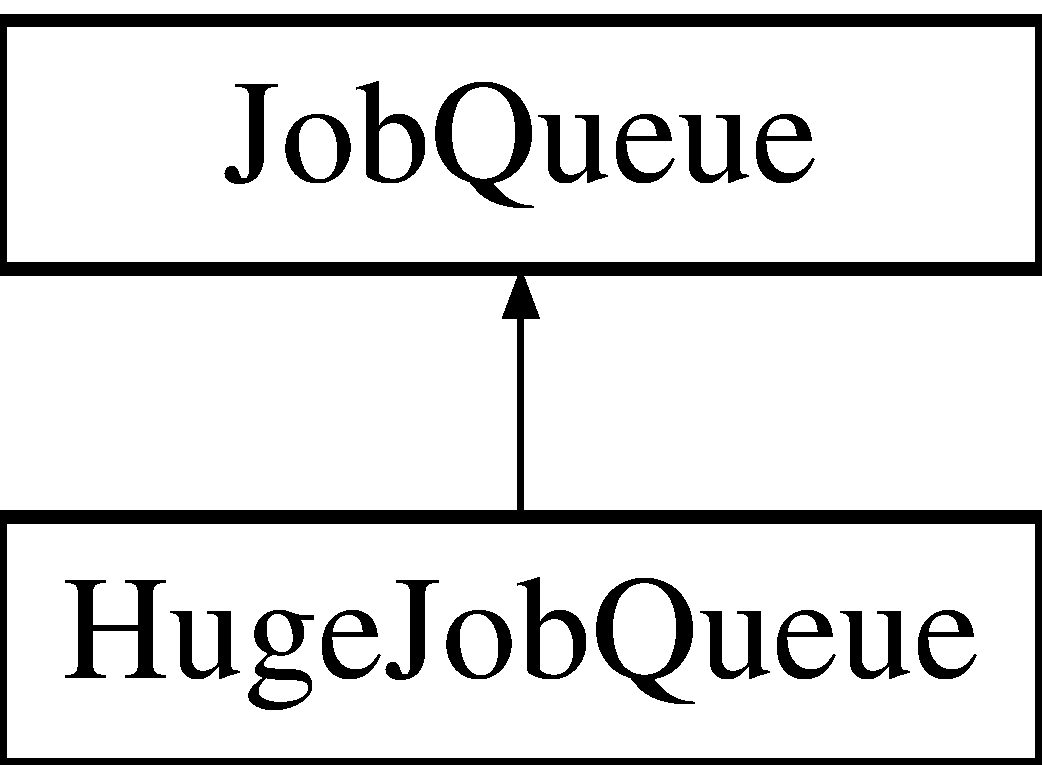
\includegraphics[height=2.000000cm]{class_huge_job_queue}
\end{center}
\end{figure}
\subsection*{Additional Inherited Members}


The documentation for this class was generated from the following files\+:\begin{DoxyCompactItemize}
\item 
D\+:/\+Cranfield work/\+Requirements Analysis and System Design/simulator project/\+Source\+Code/Huge\+Job\+Queue.\+h\item 
D\+:/\+Cranfield work/\+Requirements Analysis and System Design/simulator project/\+Source\+Code/Huge\+Job\+Queue.\+cpp\end{DoxyCompactItemize}

\hypertarget{class_input}{}\section{Input Class Reference}
\label{class_input}\index{Input@{Input}}
\subsection*{Public Member Functions}
\begin{DoxyCompactItemize}
\item 
\mbox{\Hypertarget{class_input_a1ee522db7c8b3cc5507e62d057ca5752}\label{class_input_a1ee522db7c8b3cc5507e62d057ca5752}} 
void {\bfseries time\+Step} (int time, \mbox{\hyperlink{class_users_generator}{Users\+Generator}} \&ug, \mbox{\hyperlink{class_scheduler}{Scheduler}} \&sch, \mbox{\hyperlink{class_node}{Node}} \&node)
\item 
\mbox{\Hypertarget{class_input_a12350cbbc8bcdcaf38bfc3562b7f4a97}\label{class_input_a12350cbbc8bcdcaf38bfc3562b7f4a97}} 
void {\bfseries start\+Jobs\+In\+Job\+Queue} (int time, \mbox{\hyperlink{class_users_generator}{Users\+Generator}} \&ug, \mbox{\hyperlink{class_scheduler}{Scheduler}} \&sch, \mbox{\hyperlink{class_node}{Node}} \&node, \mbox{\hyperlink{class_job_queue}{Job\+Queue}} \&jq)
\item 
\mbox{\Hypertarget{class_input_a5572ea662861b5f294195782ad953bf1}\label{class_input_a5572ea662861b5f294195782ad953bf1}} 
int {\bfseries get\+Nb\+Of\+Nodes} (\mbox{\hyperlink{class_node}{Node}} \&node, \mbox{\hyperlink{class_job_queue}{Job\+Queue}} \&jq)
\item 
\mbox{\Hypertarget{class_input_af91640b0926d1c88baae2561c1aadc5f}\label{class_input_af91640b0926d1c88baae2561c1aadc5f}} 
int {\bfseries get\+Nb\+Of\+Hours} (int type\+Of\+Queue, \mbox{\hyperlink{class_job_queue}{Job\+Queue}} \&jq)
\item 
\mbox{\Hypertarget{class_input_afa75d3fd99706a00c2847a324fefcd92}\label{class_input_afa75d3fd99706a00c2847a324fefcd92}} 
int {\bfseries get\+Type\+Of\+Nodes} ()
\item 
\mbox{\Hypertarget{class_input_ad4c4aa38487074bee3503ee4b8b40ef8}\label{class_input_ad4c4aa38487074bee3503ee4b8b40ef8}} 
double {\bfseries generate\+Number\+From\+Exponential\+Distribution} (double lambda)
\item 
\mbox{\Hypertarget{class_input_a2773675737b827a2f55d482b06fbcfd1}\label{class_input_a2773675737b827a2f55d482b06fbcfd1}} 
void {\bfseries print\+Numbers\+From\+Exponential\+Distribution} (double lambda, int iterations)
\end{DoxyCompactItemize}


The documentation for this class was generated from the following files\+:\begin{DoxyCompactItemize}
\item 
D\+:/\+Cranfield work/\+Requirements Analysis and System Design/simulator project/\+Source\+Code/Input.\+h\item 
D\+:/\+Cranfield work/\+Requirements Analysis and System Design/simulator project/\+Source\+Code/Input.\+cpp\end{DoxyCompactItemize}

\hypertarget{class_i_t_staff}{}\section{I\+T\+Staff Class Reference}
\label{class_i_t_staff}\index{I\+T\+Staff@{I\+T\+Staff}}
Inheritance diagram for I\+T\+Staff\+:\begin{figure}[H]
\begin{center}
\leavevmode
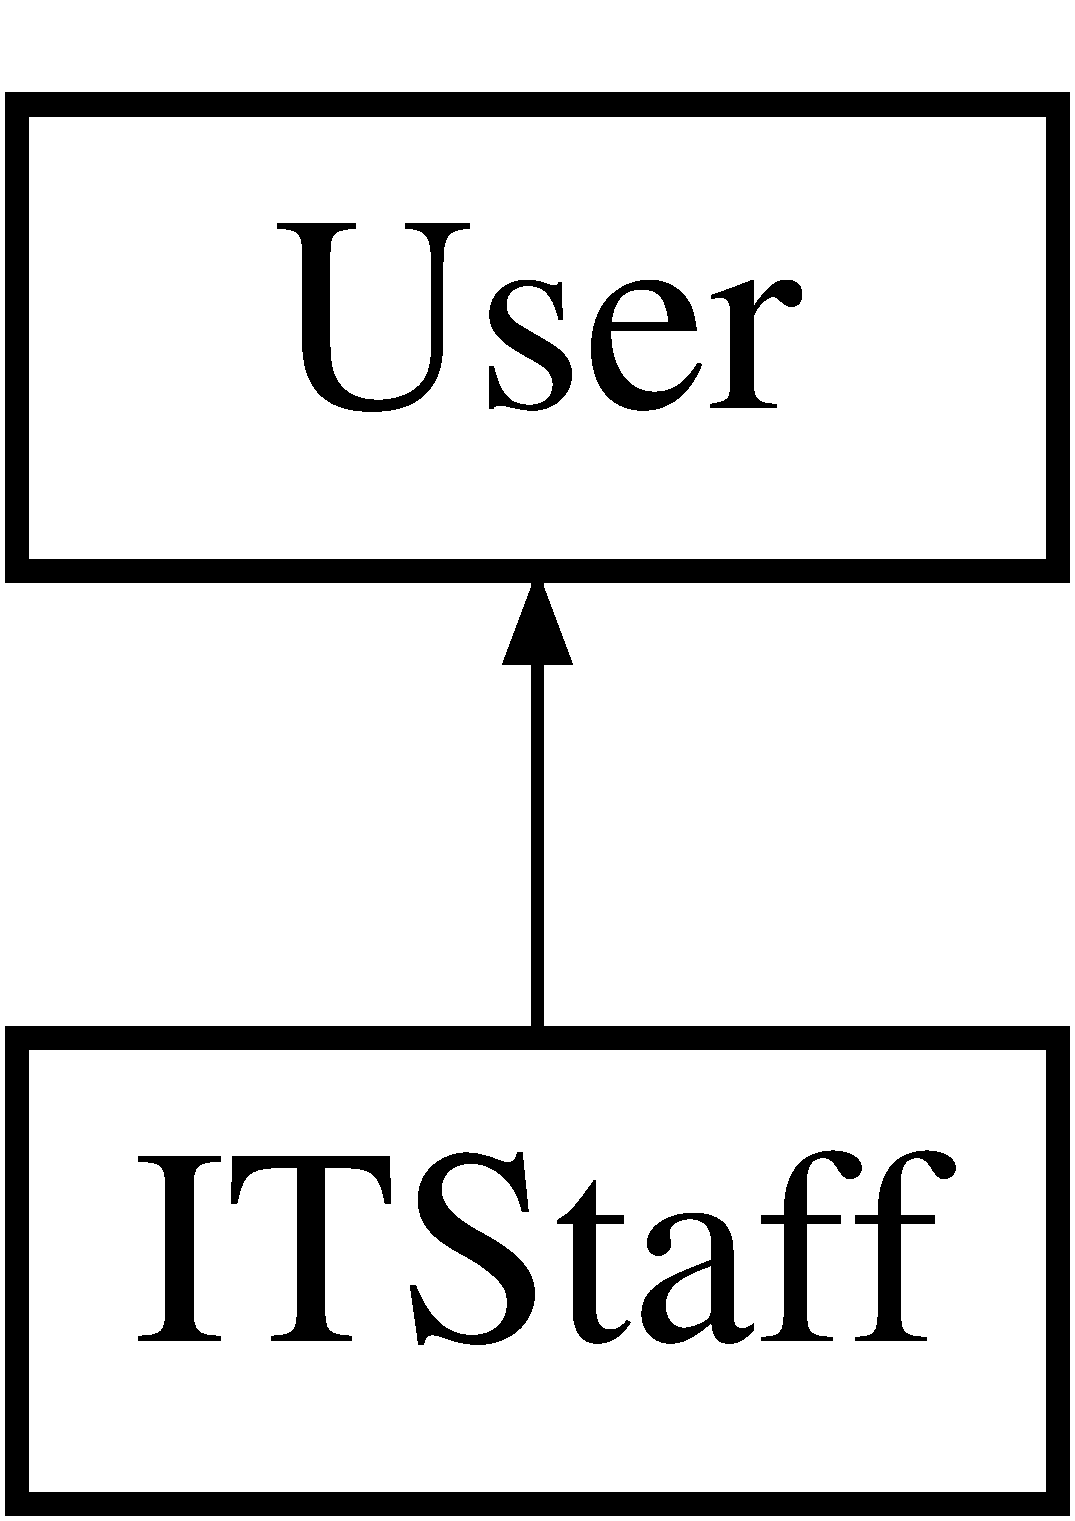
\includegraphics[height=2.000000cm]{class_i_t_staff}
\end{center}
\end{figure}
\subsection*{Public Member Functions}
\begin{DoxyCompactItemize}
\item 
\mbox{\Hypertarget{class_i_t_staff_a25ca02a72692ff5ed0c97f0c23415381}\label{class_i_t_staff_a25ca02a72692ff5ed0c97f0c23415381}} 
{\bfseries I\+T\+Staff} (int new\+Budget, int newid, double cap=1680.\+0)
\end{DoxyCompactItemize}


The documentation for this class was generated from the following files\+:\begin{DoxyCompactItemize}
\item 
D\+:/\+Cranfield work/\+Requirements Analysis and System Design/simulator project/\+Source\+Code/I\+T\+Staff.\+h\item 
D\+:/\+Cranfield work/\+Requirements Analysis and System Design/simulator project/\+Source\+Code/I\+T\+Staff.\+cpp\end{DoxyCompactItemize}

\hypertarget{class_job}{}\section{Job Class Reference}
\label{class_job}\index{Job@{Job}}
\subsection*{Public Member Functions}
\begin{DoxyCompactItemize}
\item 
\mbox{\Hypertarget{class_job_a47efbc618f9062b60684f79600d985d8}\label{class_job_a47efbc618f9062b60684f79600d985d8}} 
{\bfseries Job} (double job\+Budget, int nb\+Of\+Nodes, int nb\+Of\+Hours, int type\+Node, int user\+Id)
\end{DoxyCompactItemize}
\subsection*{Public Attributes}
\begin{DoxyCompactItemize}
\item 
\mbox{\Hypertarget{class_job_af31fad3ece1ef31d18d79435b8d002dc}\label{class_job_af31fad3ece1ef31d18d79435b8d002dc}} 
double {\bfseries budget}
\item 
\mbox{\Hypertarget{class_job_ae09a41715c749301bf627184d554a1d4}\label{class_job_ae09a41715c749301bf627184d554a1d4}} 
int {\bfseries nb\+Nodes}
\item 
\mbox{\Hypertarget{class_job_a6319e0142efd380b45893f719856823e}\label{class_job_a6319e0142efd380b45893f719856823e}} 
int {\bfseries nb\+Hours}
\item 
\mbox{\Hypertarget{class_job_a1aa451e277ebcc805a277dee15d34d44}\label{class_job_a1aa451e277ebcc805a277dee15d34d44}} 
int {\bfseries type\+Of\+Node}
\end{DoxyCompactItemize}


The documentation for this class was generated from the following files\+:\begin{DoxyCompactItemize}
\item 
D\+:/\+Cranfield work/\+Requirements Analysis and System Design/simulator project/\+Source\+Code/Job.\+h\item 
D\+:/\+Cranfield work/\+Requirements Analysis and System Design/simulator project/\+Source\+Code/Job.\+cpp\end{DoxyCompactItemize}

\hypertarget{class_job_queue}{}\section{Job\+Queue Class Reference}
\label{class_job_queue}\index{Job\+Queue@{Job\+Queue}}
Inheritance diagram for Job\+Queue\+:\begin{figure}[H]
\begin{center}
\leavevmode
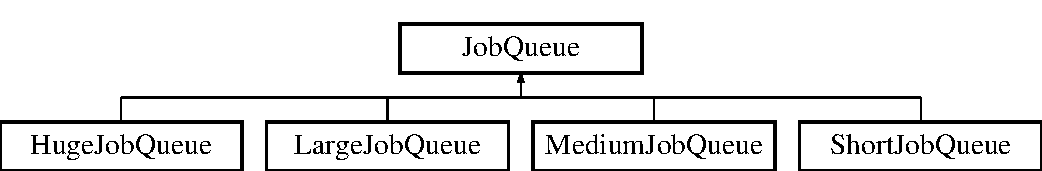
\includegraphics[height=2.000000cm]{class_job_queue}
\end{center}
\end{figure}
\subsection*{Public Member Functions}
\begin{DoxyCompactItemize}
\item 
\mbox{\Hypertarget{class_job_queue_a6d530bf47827ca5b7fd1733908206d9d}\label{class_job_queue_a6d530bf47827ca5b7fd1733908206d9d}} 
vector$<$ \mbox{\hyperlink{class_job}{Job}} $>$ {\bfseries get\+Job\+Queue} ()
\item 
\mbox{\Hypertarget{class_job_queue_aa21eaa87e05aca2ff536effe4fae1f36}\label{class_job_queue_aa21eaa87e05aca2ff536effe4fae1f36}} 
void {\bfseries add\+To\+Job\+Queue} (\mbox{\hyperlink{class_job}{Job}} job)
\item 
\mbox{\Hypertarget{class_job_queue_a40acca49c00bd568337e5e99cee2c936}\label{class_job_queue_a40acca49c00bd568337e5e99cee2c936}} 
void {\bfseries remove\+From\+Job\+Queue} (int i)
\item 
\mbox{\Hypertarget{class_job_queue_a337fbbcbcd9fdc0d7b4cdf1445540eeb}\label{class_job_queue_a337fbbcbcd9fdc0d7b4cdf1445540eeb}} 
void {\bfseries number\+Of\+Jobs\+Processed\+Plus1} ()
\item 
\mbox{\Hypertarget{class_job_queue_a82772a0000d5ad7380950c88c8718d01}\label{class_job_queue_a82772a0000d5ad7380950c88c8718d01}} 
void {\bfseries add\+New\+Wait\+Time} (int time\+Waited)
\item 
\mbox{\Hypertarget{class_job_queue_ad410dafe929327135889e271bd6a2d23}\label{class_job_queue_ad410dafe929327135889e271bd6a2d23}} 
void {\bfseries add\+New\+Run\+Time} (int time\+Run)
\item 
\mbox{\Hypertarget{class_job_queue_a38e08b929dda86f26a29c2c013905b74}\label{class_job_queue_a38e08b929dda86f26a29c2c013905b74}} 
double {\bfseries get\+Average\+Wait\+Time} ()
\item 
\mbox{\Hypertarget{class_job_queue_a3c386ff5559788ce23ee86dc2b69c93b}\label{class_job_queue_a3c386ff5559788ce23ee86dc2b69c93b}} 
double {\bfseries get\+Average\+Run\+Time} ()
\item 
\mbox{\Hypertarget{class_job_queue_a4965c12a271ee4cb1c9fadfcee2b51d3}\label{class_job_queue_a4965c12a271ee4cb1c9fadfcee2b51d3}} 
double {\bfseries get\+Average\+Turnaround\+Time\+Ratio} ()
\end{DoxyCompactItemize}
\subsection*{Public Attributes}
\begin{DoxyCompactItemize}
\item 
\mbox{\Hypertarget{class_job_queue_a2df2ae8313ca2248d59f68158fa64de5}\label{class_job_queue_a2df2ae8313ca2248d59f68158fa64de5}} 
vector$<$ \mbox{\hyperlink{class_job}{Job}} $>$ {\bfseries job\+Queue\+Vector}
\item 
\mbox{\Hypertarget{class_job_queue_abcf8363998ac230e81b6e84d13a0da05}\label{class_job_queue_abcf8363998ac230e81b6e84d13a0da05}} 
double {\bfseries cost\+Per\+Machine\+Hour}
\item 
\mbox{\Hypertarget{class_job_queue_aa14e93d8289f0cbffdd1e7fdb5991e00}\label{class_job_queue_aa14e93d8289f0cbffdd1e7fdb5991e00}} 
int {\bfseries max\+Nb\+Of\+Hours}
\item 
\mbox{\Hypertarget{class_job_queue_aec23b24c5671b66aeb8bcb619f390ab9}\label{class_job_queue_aec23b24c5671b66aeb8bcb619f390ab9}} 
int {\bfseries max\+Nb\+Of\+Nodes}
\item 
\mbox{\Hypertarget{class_job_queue_aee18b3b19b0faf073e1399a3725d92f7}\label{class_job_queue_aee18b3b19b0faf073e1399a3725d92f7}} 
int {\bfseries number\+Of\+Jobs\+Processed}
\item 
\mbox{\Hypertarget{class_job_queue_acc66a3f47ac7bbec772f0c5ea5d699c3}\label{class_job_queue_acc66a3f47ac7bbec772f0c5ea5d699c3}} 
vector$<$ int $>$ {\bfseries wait\+Time}
\item 
\mbox{\Hypertarget{class_job_queue_a3a9b97d1a3b1ee0da81747335a0a5d25}\label{class_job_queue_a3a9b97d1a3b1ee0da81747335a0a5d25}} 
vector$<$ int $>$ {\bfseries run\+Time}
\item 
\mbox{\Hypertarget{class_job_queue_ab6876a626f1767a5bb7e63a65ce1faef}\label{class_job_queue_ab6876a626f1767a5bb7e63a65ce1faef}} 
double {\bfseries lambda}
\item 
\mbox{\Hypertarget{class_job_queue_a2b9e866b703b97a2fcec2ef289a1f00a}\label{class_job_queue_a2b9e866b703b97a2fcec2ef289a1f00a}} 
int {\bfseries exponential\+Distribution\+Factor}
\end{DoxyCompactItemize}


The documentation for this class was generated from the following files\+:\begin{DoxyCompactItemize}
\item 
D\+:/\+Cranfield work/\+Requirements Analysis and System Design/simulator project/\+Source\+Code/Job\+Queue.\+h\item 
D\+:/\+Cranfield work/\+Requirements Analysis and System Design/simulator project/\+Source\+Code/Job\+Queue.\+cpp\end{DoxyCompactItemize}

\hypertarget{class_large_job_queue}{}\section{Large\+Job\+Queue Class Reference}
\label{class_large_job_queue}\index{Large\+Job\+Queue@{Large\+Job\+Queue}}
Inheritance diagram for Large\+Job\+Queue\+:\begin{figure}[H]
\begin{center}
\leavevmode
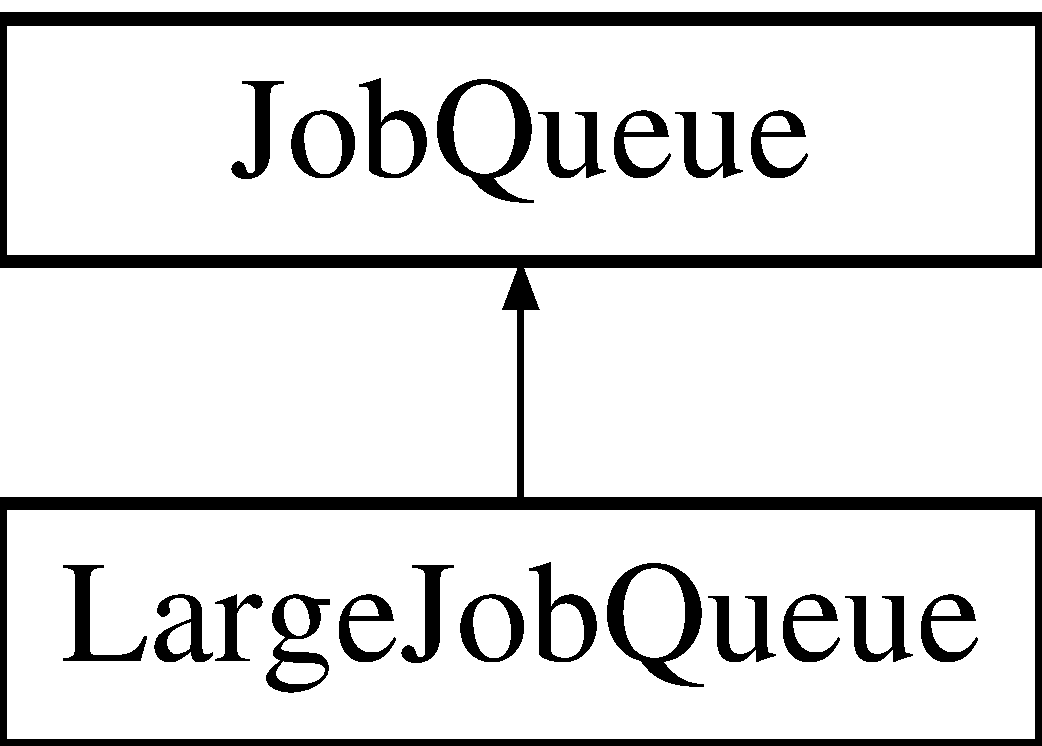
\includegraphics[height=2.000000cm]{class_large_job_queue}
\end{center}
\end{figure}
\subsection*{Additional Inherited Members}


The documentation for this class was generated from the following files\+:\begin{DoxyCompactItemize}
\item 
D\+:/\+Cranfield work/\+Requirements Analysis and System Design/simulator project/\+Source\+Code/Large\+Job\+Queue.\+h\item 
D\+:/\+Cranfield work/\+Requirements Analysis and System Design/simulator project/\+Source\+Code/Large\+Job\+Queue.\+cpp\end{DoxyCompactItemize}

\hypertarget{class_medium_job_queue}{}\section{Medium\+Job\+Queue Class Reference}
\label{class_medium_job_queue}\index{Medium\+Job\+Queue@{Medium\+Job\+Queue}}
Inheritance diagram for Medium\+Job\+Queue\+:\begin{figure}[H]
\begin{center}
\leavevmode
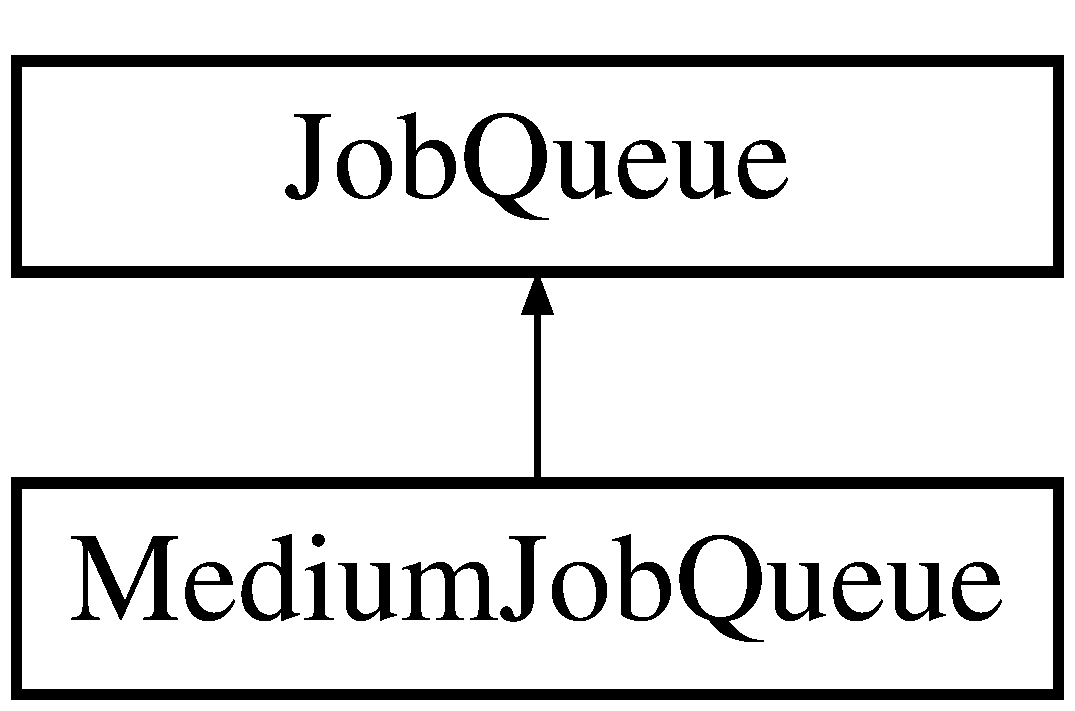
\includegraphics[height=2.000000cm]{class_medium_job_queue}
\end{center}
\end{figure}
\subsection*{Additional Inherited Members}


The documentation for this class was generated from the following files\+:\begin{DoxyCompactItemize}
\item 
D\+:/\+Cranfield work/\+Requirements Analysis and System Design/simulator project/\+Source\+Code/Medium\+Job\+Queue.\+h\item 
D\+:/\+Cranfield work/\+Requirements Analysis and System Design/simulator project/\+Source\+Code/Medium\+Job\+Queue.\+cpp\end{DoxyCompactItemize}

\hypertarget{class_node}{}\section{Node Class Reference}
\label{class_node}\index{Node@{Node}}
\subsection*{Public Member Functions}
\begin{DoxyCompactItemize}
\item 
\mbox{\Hypertarget{class_node_a9b392d27de54c97ef230c6f96975ec86}\label{class_node_a9b392d27de54c97ef230c6f96975ec86}} 
{\bfseries Node} (int nb\+Traditional\+Nodes=64, int nb\+Accelerated\+Nodes=32, int nb\+Specialized\+Nodes=32)
\item 
\mbox{\Hypertarget{class_node_a8ea7618f3d3c911f41befaf771c94c55}\label{class_node_a8ea7618f3d3c911f41befaf771c94c55}} 
void {\bfseries use\+Nodes} (Matrix \&nodes, int start\+Time, int nb\+Of\+Nodes, \mbox{\hyperlink{class_job_queue}{Job\+Queue}} \&job\+Queue)
\item 
\mbox{\Hypertarget{class_node_a429132bde9ec23913d9dfab4ffd23971}\label{class_node_a429132bde9ec23913d9dfab4ffd23971}} 
int {\bfseries get\+Total\+Number\+Of\+Machine\+Hours\+Consumed} ()
\end{DoxyCompactItemize}
\subsection*{Public Attributes}
\begin{DoxyCompactItemize}
\item 
\mbox{\Hypertarget{class_node_ab3c28d4dffc8911009b7af4b079ce99f}\label{class_node_ab3c28d4dffc8911009b7af4b079ce99f}} 
int {\bfseries nb\+Of\+Hours\+Per\+Week}
\item 
\mbox{\Hypertarget{class_node_a6bb2fba37331b31a5b57cba59ed34406}\label{class_node_a6bb2fba37331b31a5b57cba59ed34406}} 
int {\bfseries nb\+Of\+Traditional\+Nodes}
\item 
\mbox{\Hypertarget{class_node_a7065d23d72c9395a4c04462d70885c1b}\label{class_node_a7065d23d72c9395a4c04462d70885c1b}} 
int {\bfseries nb\+Of\+Accelerated\+Nodes}
\item 
\mbox{\Hypertarget{class_node_afb2cc27b3b3385f9d0bbc4f21a330841}\label{class_node_afb2cc27b3b3385f9d0bbc4f21a330841}} 
int {\bfseries nb\+Of\+Specialized\+Nodes}
\item 
\mbox{\Hypertarget{class_node_adeb696381aeabb3622f46ee44d0f5418}\label{class_node_adeb696381aeabb3622f46ee44d0f5418}} 
Matrix {\bfseries traditional\+Nodes}
\item 
\mbox{\Hypertarget{class_node_acfc5a971c0d55eebd3b9b487936263c6}\label{class_node_acfc5a971c0d55eebd3b9b487936263c6}} 
Matrix {\bfseries accelerated\+Nodes}
\item 
\mbox{\Hypertarget{class_node_ae46791f9ae6fbbaa5f16e4d6380b200d}\label{class_node_ae46791f9ae6fbbaa5f16e4d6380b200d}} 
Matrix {\bfseries specialized\+Nodes}
\end{DoxyCompactItemize}


The documentation for this class was generated from the following files\+:\begin{DoxyCompactItemize}
\item 
D\+:/\+Cranfield work/\+Requirements Analysis and System Design/simulator project/\+Source\+Code/Node.\+h\item 
D\+:/\+Cranfield work/\+Requirements Analysis and System Design/simulator project/\+Source\+Code/Node.\+cpp\end{DoxyCompactItemize}

\hypertarget{class_output}{}\section{Output Class Reference}
\label{class_output}\index{Output@{Output}}
\subsection*{Public Member Functions}
\begin{DoxyCompactItemize}
\item 
\mbox{\Hypertarget{class_output_acb9d8ee43f81560de2beec11bf8983bf}\label{class_output_acb9d8ee43f81560de2beec11bf8983bf}} 
void {\bfseries output\+Results\+Of\+The\+Simulation} (\mbox{\hyperlink{class_scheduler}{Scheduler}} \&sch, \mbox{\hyperlink{class_node}{Node}} \&node, \mbox{\hyperlink{class_users_generator}{Users\+Generator}} \&ug, int number\+Of\+Machine\+Hours\+Available, double operating\+Cost)
\item 
\mbox{\Hypertarget{class_output_a37b5da24dd73ba9c7fbc1d70807ee59a}\label{class_output_a37b5da24dd73ba9c7fbc1d70807ee59a}} 
void {\bfseries number\+Of\+Jobs\+Processed\+In\+Each\+Queue} (\mbox{\hyperlink{class_scheduler}{Scheduler}} \&sch)
\item 
\mbox{\Hypertarget{class_output_a17c8f535b597f35ae4756695aed70da4}\label{class_output_a17c8f535b597f35ae4756695aed70da4}} 
void {\bfseries actual\+Number\+Of\+Machine\+Hours\+Consumed\+By\+Each\+Job} (\mbox{\hyperlink{class_scheduler}{Scheduler}} \&sch)
\item 
\mbox{\Hypertarget{class_output_aeae2d017558edea58d43914e9601600c}\label{class_output_aeae2d017558edea58d43914e9601600c}} 
void {\bfseries utilization\+Ratio} (\mbox{\hyperlink{class_node}{Node}} \&node, int number\+Of\+Machine\+Hours\+Available)
\item 
\mbox{\Hypertarget{class_output_a0195b7d1a95f2a5d7ae4fc84f513ce58}\label{class_output_a0195b7d1a95f2a5d7ae4fc84f513ce58}} 
void {\bfseries price\+Paid\+By\+The\+Users} (\mbox{\hyperlink{class_users_generator}{Users\+Generator}} \&ug)
\item 
\mbox{\Hypertarget{class_output_a0d052cfab8080543ea59abf505523d27}\label{class_output_a0d052cfab8080543ea59abf505523d27}} 
void {\bfseries average\+Wait\+Time\+In\+Each\+Queue} (\mbox{\hyperlink{class_scheduler}{Scheduler}} \&sch)
\item 
\mbox{\Hypertarget{class_output_ac9a0aeeefa8ef13cf8849487ea0133be}\label{class_output_ac9a0aeeefa8ef13cf8849487ea0133be}} 
void {\bfseries average\+Turnaround\+Time\+Ratio} (\mbox{\hyperlink{class_scheduler}{Scheduler}} \&sch)
\item 
\mbox{\Hypertarget{class_output_a3adb2cfe1229a1267fe8160ab70c562e}\label{class_output_a3adb2cfe1229a1267fe8160ab70c562e}} 
void {\bfseries economic\+Balance\+Of\+The\+Centre} (\mbox{\hyperlink{class_users_generator}{Users\+Generator}} \&ug, double operating\+Cost)
\item 
\mbox{\Hypertarget{class_output_a536b72eb2ce4b4bc2b15b315e823be92}\label{class_output_a536b72eb2ce4b4bc2b15b315e823be92}} 
void {\bfseries show\+Traditional\+Nodes} (\mbox{\hyperlink{class_node}{Node}} \&node)
\item 
\mbox{\Hypertarget{class_output_a10c9b770f51f6809f8d1da04fa88aa2e}\label{class_output_a10c9b770f51f6809f8d1da04fa88aa2e}} 
void {\bfseries show\+Accelerated\+Nodes} (\mbox{\hyperlink{class_node}{Node}} \&node)
\item 
\mbox{\Hypertarget{class_output_a2e26fc88b8088a4cae12b7e6854992a6}\label{class_output_a2e26fc88b8088a4cae12b7e6854992a6}} 
void {\bfseries show\+Specialized\+Nodes} (\mbox{\hyperlink{class_node}{Node}} \&node)
\item 
\mbox{\Hypertarget{class_output_a063064bb29bc5b4de55705960785feff}\label{class_output_a063064bb29bc5b4de55705960785feff}} 
void {\bfseries show\+Nodes} (Matrix \&nodes)
\end{DoxyCompactItemize}


The documentation for this class was generated from the following files\+:\begin{DoxyCompactItemize}
\item 
D\+:/\+Cranfield work/\+Requirements Analysis and System Design/simulator project/\+Source\+Code/Output.\+h\item 
D\+:/\+Cranfield work/\+Requirements Analysis and System Design/simulator project/\+Source\+Code/Output.\+cpp\end{DoxyCompactItemize}

\hypertarget{class_researcher}{}\section{Researcher Class Reference}
\label{class_researcher}\index{Researcher@{Researcher}}
Inheritance diagram for Researcher\+:\begin{figure}[H]
\begin{center}
\leavevmode
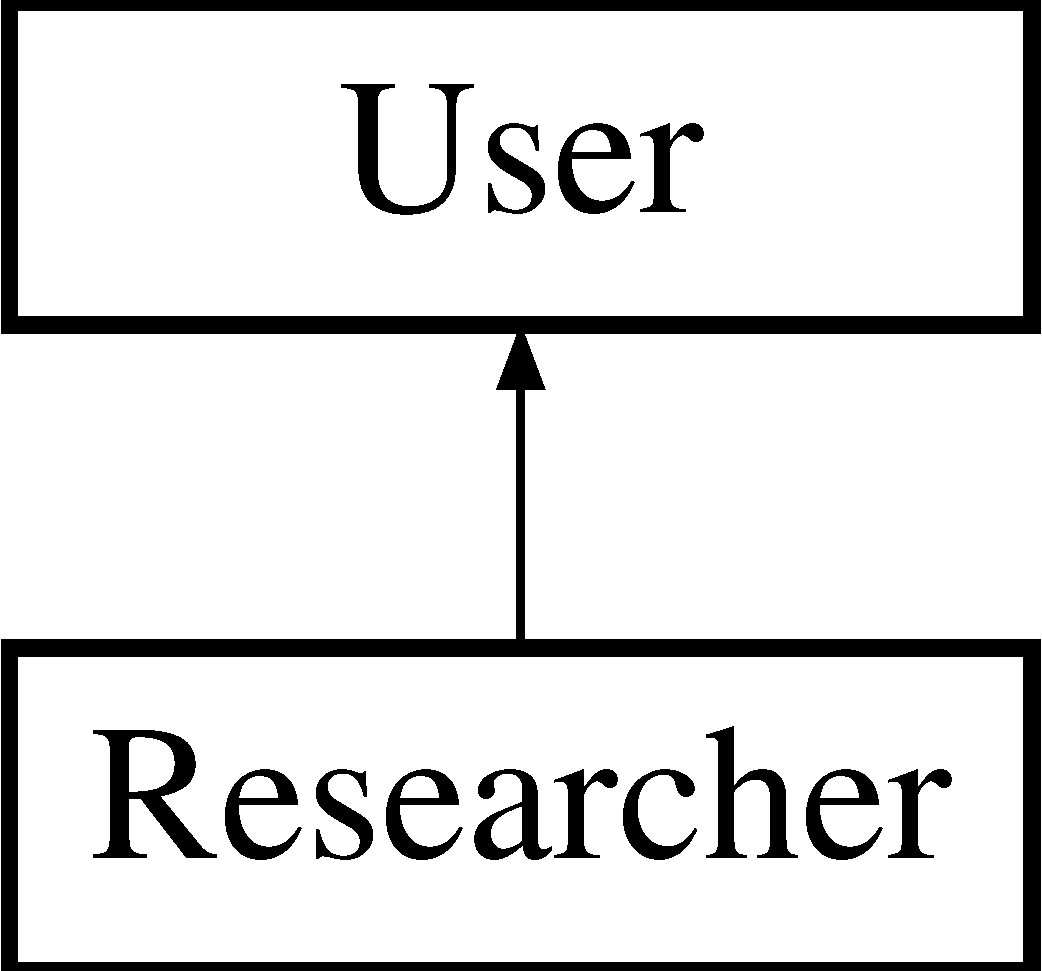
\includegraphics[height=2.000000cm]{class_researcher}
\end{center}
\end{figure}
\subsection*{Public Member Functions}
\begin{DoxyCompactItemize}
\item 
\mbox{\Hypertarget{class_researcher_a9c851cb4b8427bf22d4658df25ebcd02}\label{class_researcher_a9c851cb4b8427bf22d4658df25ebcd02}} 
{\bfseries Researcher} (int new\+Budget, int newid, double cap=1600.\+0)
\end{DoxyCompactItemize}


The documentation for this class was generated from the following files\+:\begin{DoxyCompactItemize}
\item 
D\+:/\+Cranfield work/\+Requirements Analysis and System Design/simulator project/\+Source\+Code/Researcher.\+h\item 
D\+:/\+Cranfield work/\+Requirements Analysis and System Design/simulator project/\+Source\+Code/Researcher.\+cpp\end{DoxyCompactItemize}

\hypertarget{class_scheduler}{}\section{Scheduler Class Reference}
\label{class_scheduler}\index{Scheduler@{Scheduler}}
\subsection*{Public Member Functions}
\begin{DoxyCompactItemize}
\item 
\mbox{\Hypertarget{class_scheduler_a9a97c1e371779013d1f391047831132b}\label{class_scheduler_a9a97c1e371779013d1f391047831132b}} 
void {\bfseries treat\+Job\+In\+Queue} (\mbox{\hyperlink{class_job_queue}{Job\+Queue}} \&job\+Queue, \mbox{\hyperlink{class_node}{Node}} \&node, int time)
\end{DoxyCompactItemize}
\subsection*{Public Attributes}
\begin{DoxyCompactItemize}
\item 
\mbox{\Hypertarget{class_scheduler_a230bcf2e686da11204241df858aee185}\label{class_scheduler_a230bcf2e686da11204241df858aee185}} 
\mbox{\hyperlink{class_short_job_queue}{Short\+Job\+Queue}} {\bfseries sjq}
\item 
\mbox{\Hypertarget{class_scheduler_a64b5c8f9d4801e0ce53b20a3915ba72a}\label{class_scheduler_a64b5c8f9d4801e0ce53b20a3915ba72a}} 
\mbox{\hyperlink{class_medium_job_queue}{Medium\+Job\+Queue}} {\bfseries mjq}
\item 
\mbox{\Hypertarget{class_scheduler_a235ae26896fab67995f166678bf0b506}\label{class_scheduler_a235ae26896fab67995f166678bf0b506}} 
\mbox{\hyperlink{class_large_job_queue}{Large\+Job\+Queue}} {\bfseries ljq}
\item 
\mbox{\Hypertarget{class_scheduler_a6f057765dd7084c1b0f37517eb90fcdb}\label{class_scheduler_a6f057765dd7084c1b0f37517eb90fcdb}} 
\mbox{\hyperlink{class_huge_job_queue}{Huge\+Job\+Queue}} {\bfseries hjq}
\item 
\mbox{\Hypertarget{class_scheduler_a14db1ba2a7ea1e676e75bd254e0418a4}\label{class_scheduler_a14db1ba2a7ea1e676e75bd254e0418a4}} 
vector$<$ int $>$ {\bfseries number\+Of\+Machine\+Hours\+Consumed}
\end{DoxyCompactItemize}


The documentation for this class was generated from the following files\+:\begin{DoxyCompactItemize}
\item 
D\+:/\+Cranfield work/\+Requirements Analysis and System Design/simulator project/\+Source\+Code/Scheduler.\+h\item 
D\+:/\+Cranfield work/\+Requirements Analysis and System Design/simulator project/\+Source\+Code/Scheduler.\+cpp\end{DoxyCompactItemize}

\hypertarget{class_short_job_queue}{}\section{Short\+Job\+Queue Class Reference}
\label{class_short_job_queue}\index{Short\+Job\+Queue@{Short\+Job\+Queue}}
Inheritance diagram for Short\+Job\+Queue\+:\begin{figure}[H]
\begin{center}
\leavevmode
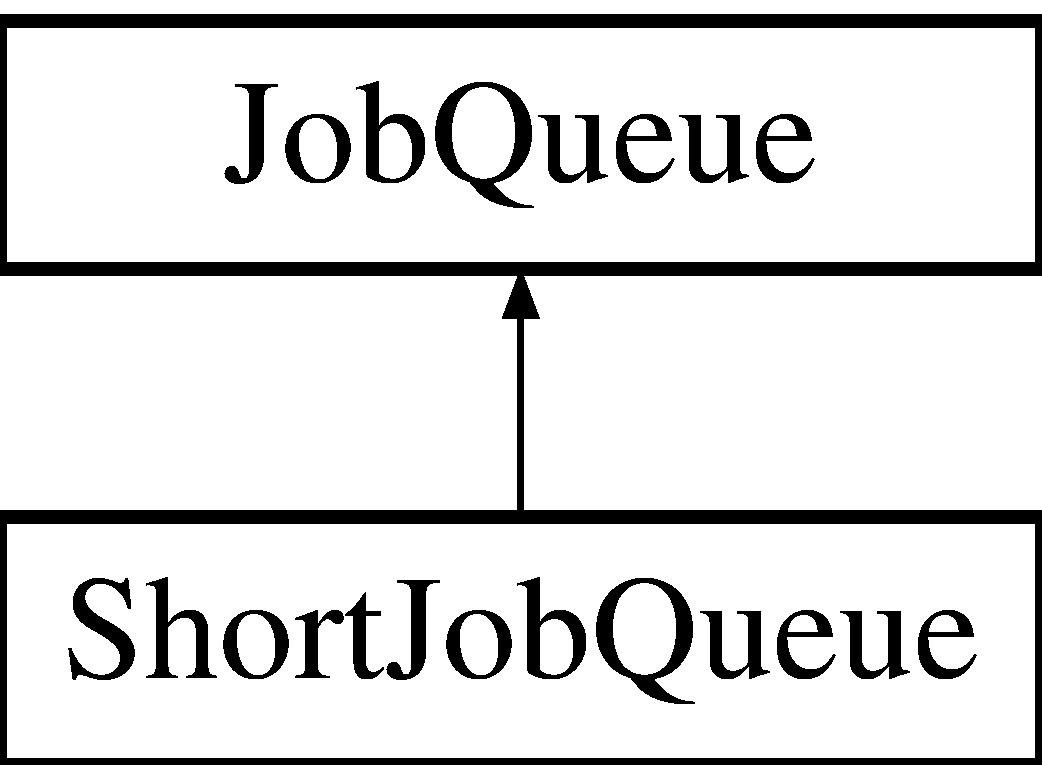
\includegraphics[height=2.000000cm]{class_short_job_queue}
\end{center}
\end{figure}
\subsection*{Additional Inherited Members}


The documentation for this class was generated from the following files\+:\begin{DoxyCompactItemize}
\item 
D\+:/\+Cranfield work/\+Requirements Analysis and System Design/simulator project/\+Source\+Code/Short\+Job\+Queue.\+h\item 
D\+:/\+Cranfield work/\+Requirements Analysis and System Design/simulator project/\+Source\+Code/Short\+Job\+Queue.\+cpp\end{DoxyCompactItemize}

\hypertarget{class_student}{}\section{Student Class Reference}
\label{class_student}\index{Student@{Student}}
Inheritance diagram for Student\+:\begin{figure}[H]
\begin{center}
\leavevmode
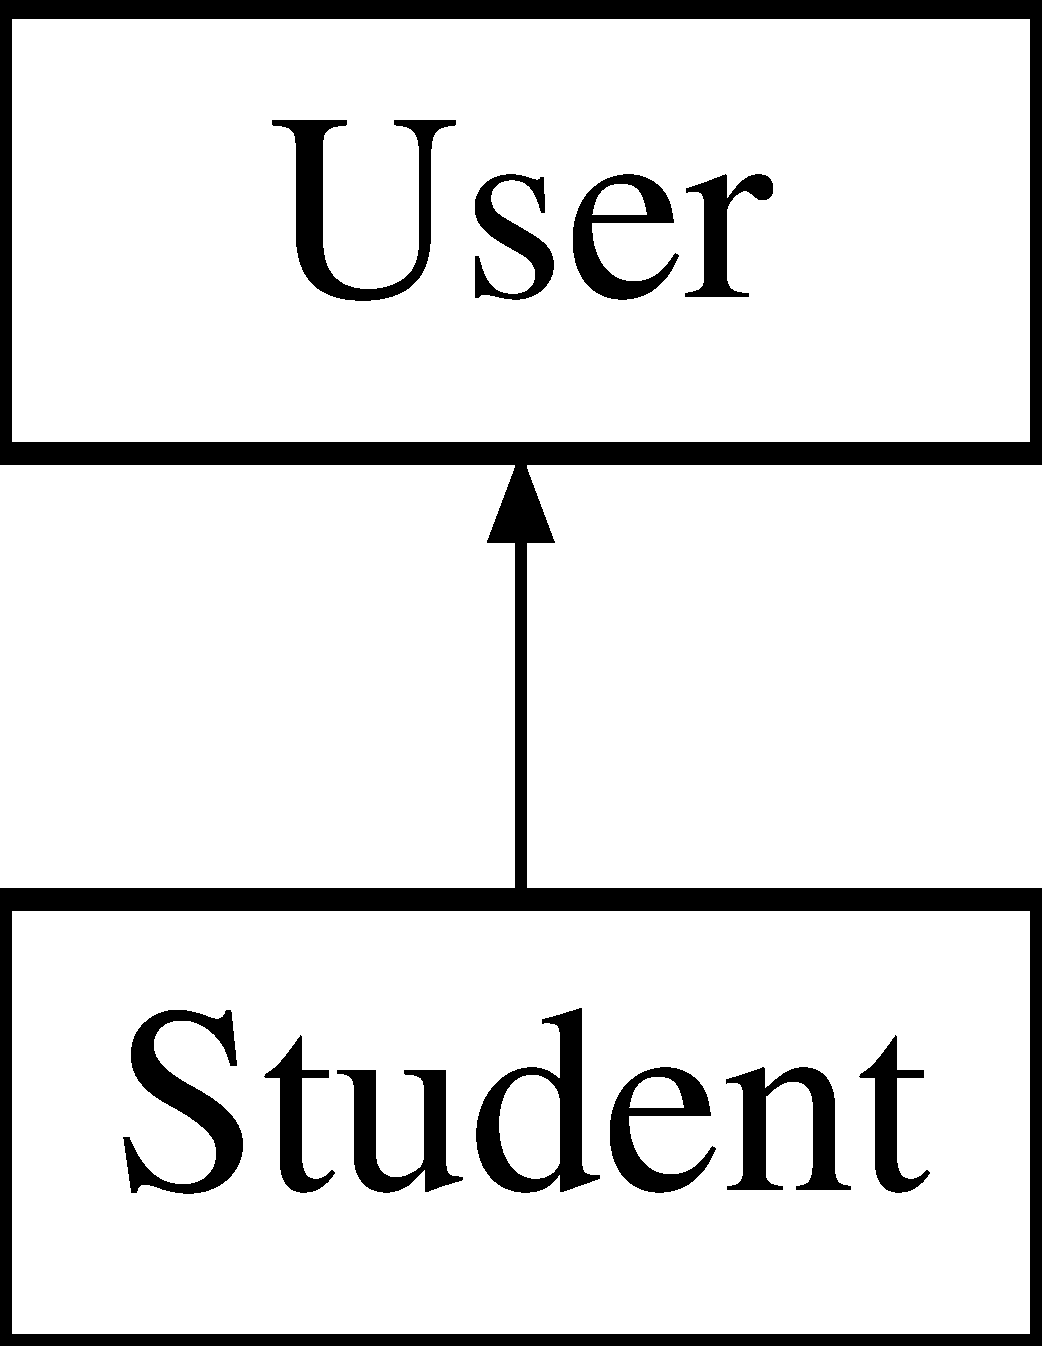
\includegraphics[height=2.000000cm]{class_student}
\end{center}
\end{figure}
\subsection*{Public Member Functions}
\begin{DoxyCompactItemize}
\item 
\mbox{\Hypertarget{class_student_a2d774a1d93be9037e9fcbda9750b9e33}\label{class_student_a2d774a1d93be9037e9fcbda9750b9e33}} 
{\bfseries Student} (int new\+Budget, int newid, double cap=100.\+0)
\end{DoxyCompactItemize}


The documentation for this class was generated from the following files\+:\begin{DoxyCompactItemize}
\item 
D\+:/\+Cranfield work/\+Requirements Analysis and System Design/simulator project/\+Source\+Code/Student.\+h\item 
D\+:/\+Cranfield work/\+Requirements Analysis and System Design/simulator project/\+Source\+Code/Student.\+cpp\end{DoxyCompactItemize}

\hypertarget{class_test}{}\section{Test Class Reference}
\label{class_test}\index{Test@{Test}}
\subsection*{Public Member Functions}
\begin{DoxyCompactItemize}
\item 
\mbox{\Hypertarget{class_test_a97d77dce48bd99f1af0a5c3a8be8b435}\label{class_test_a97d77dce48bd99f1af0a5c3a8be8b435}} 
void {\bfseries test\+Simulation} ()
\item 
\mbox{\Hypertarget{class_test_a4901403f34d65327a6fcb50b4b4387d3}\label{class_test_a4901403f34d65327a6fcb50b4b4387d3}} 
void {\bfseries test\+Input} ()
\item 
\mbox{\Hypertarget{class_test_a4a184aa153f2df4f4840fffed926cba5}\label{class_test_a4a184aa153f2df4f4840fffed926cba5}} 
void {\bfseries test\+Output} ()
\item 
\mbox{\Hypertarget{class_test_a0c0a7237b36e554b70393e9a9afb0827}\label{class_test_a0c0a7237b36e554b70393e9a9afb0827}} 
void {\bfseries test\+Job} ()
\item 
\mbox{\Hypertarget{class_test_a6c89d0a52d3737d13e7d7d559795f7f0}\label{class_test_a6c89d0a52d3737d13e7d7d559795f7f0}} 
void {\bfseries test\+Node} ()
\item 
\mbox{\Hypertarget{class_test_a153995343cf614c7196b3d64621ae62e}\label{class_test_a153995343cf614c7196b3d64621ae62e}} 
void {\bfseries test\+Scheduler} ()
\item 
\mbox{\Hypertarget{class_test_a9bd9be841180b6597b709bba9b057e90}\label{class_test_a9bd9be841180b6597b709bba9b057e90}} 
void {\bfseries test\+Users\+Generator} ()
\item 
\mbox{\Hypertarget{class_test_ae2a4a763ae3e91b6c4b3dc21eaa84e08}\label{class_test_ae2a4a763ae3e91b6c4b3dc21eaa84e08}} 
void {\bfseries test\+Evaluator\+Of\+Scheduler} ()
\item 
\mbox{\Hypertarget{class_test_a8ead44ebf288f773db2497712989286b}\label{class_test_a8ead44ebf288f773db2497712989286b}} 
void {\bfseries test\+Job\+Queue} ()
\item 
\mbox{\Hypertarget{class_test_ad556a698bd0eb5c9717d8c3e1143369b}\label{class_test_ad556a698bd0eb5c9717d8c3e1143369b}} 
void {\bfseries test\+Huge\+Job\+Queue} ()
\item 
\mbox{\Hypertarget{class_test_a139b768530114e54813d672dd0b88388}\label{class_test_a139b768530114e54813d672dd0b88388}} 
void {\bfseries test\+Large\+Job\+Queue} ()
\item 
\mbox{\Hypertarget{class_test_a8e49cb775161256e71bda76826cc3208}\label{class_test_a8e49cb775161256e71bda76826cc3208}} 
void {\bfseries test\+Medium\+Job\+Queue} ()
\item 
\mbox{\Hypertarget{class_test_abc29314e9cf9979de46392407b891220}\label{class_test_abc29314e9cf9979de46392407b891220}} 
void {\bfseries test\+Short\+Job\+Queue} ()
\item 
\mbox{\Hypertarget{class_test_a0e61f8c2dad4fdf5d60dd98a42c9f2a9}\label{class_test_a0e61f8c2dad4fdf5d60dd98a42c9f2a9}} 
void {\bfseries test\+User} ()
\item 
\mbox{\Hypertarget{class_test_a596b84b3a78ae1ed51f307c6641b3a3a}\label{class_test_a596b84b3a78ae1ed51f307c6641b3a3a}} 
void {\bfseries test\+I\+T\+Staff} ()
\item 
\mbox{\Hypertarget{class_test_a072c839b417675b9f34d4011e7d54147}\label{class_test_a072c839b417675b9f34d4011e7d54147}} 
void {\bfseries test\+Researcher} ()
\item 
\mbox{\Hypertarget{class_test_a44ed9c72e9610a1d492533445db23a5b}\label{class_test_a44ed9c72e9610a1d492533445db23a5b}} 
void {\bfseries test\+Student} ()
\end{DoxyCompactItemize}


The documentation for this class was generated from the following files\+:\begin{DoxyCompactItemize}
\item 
D\+:/\+Cranfield work/\+Requirements Analysis and System Design/simulator project/\+Source\+Code/Test.\+h\item 
D\+:/\+Cranfield work/\+Requirements Analysis and System Design/simulator project/\+Source\+Code/Test.\+cpp\end{DoxyCompactItemize}

\hypertarget{class_user}{}\section{User Class Reference}
\label{class_user}\index{User@{User}}
Inheritance diagram for User\+:\begin{figure}[H]
\begin{center}
\leavevmode
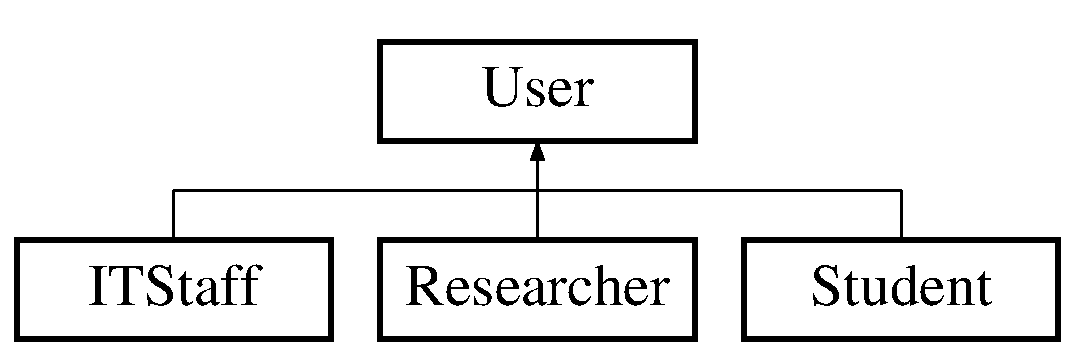
\includegraphics[height=2.000000cm]{class_user}
\end{center}
\end{figure}
\subsection*{Public Member Functions}
\begin{DoxyCompactItemize}
\item 
\mbox{\Hypertarget{class_user_ac5bc283639864f3d7f88ede4f0a8a332}\label{class_user_ac5bc283639864f3d7f88ede4f0a8a332}} 
{\bfseries User} (double user\+Budget, int user\+Id, double cap=1680.\+0)
\item 
\mbox{\Hypertarget{class_user_ae32aaa5d9ea260235599c9e4c4052046}\label{class_user_ae32aaa5d9ea260235599c9e4c4052046}} 
double {\bfseries get\+Budget} ()
\item 
\mbox{\Hypertarget{class_user_aec39d775c97e0c9f0234f45892d61f0d}\label{class_user_aec39d775c97e0c9f0234f45892d61f0d}} 
double {\bfseries get\+Budget\+Spent} ()
\item 
\mbox{\Hypertarget{class_user_a1e393732cd9838ab29445d9153333046}\label{class_user_a1e393732cd9838ab29445d9153333046}} 
int {\bfseries get\+Id} ()
\item 
\mbox{\Hypertarget{class_user_a792d82405cd2fd41f8e8b377d3f74827}\label{class_user_a792d82405cd2fd41f8e8b377d3f74827}} 
double {\bfseries get\+Instantaneous\+Cap} ()
\item 
\mbox{\Hypertarget{class_user_a842dee214d1c05758a362a5944b07cd1}\label{class_user_a842dee214d1c05758a362a5944b07cd1}} 
void {\bfseries spend\+Budget} (double budget\+User\+Spent)
\item 
\mbox{\Hypertarget{class_user_adcbf63de0acbc62bbb3c717e7652a91c}\label{class_user_adcbf63de0acbc62bbb3c717e7652a91c}} 
\mbox{\hyperlink{class_job}{Job}} {\bfseries create\+Job\+And\+Send\+Tosend\+Job\+To\+Job\+Queue} (int nb\+Of\+Nodes, int nb\+Of\+Hours, int type\+Node, \mbox{\hyperlink{class_job_queue}{Job\+Queue}} \&jobq, \mbox{\hyperlink{class_node}{Node}} \&node, int time, \mbox{\hyperlink{class_scheduler}{Scheduler}} \&sch)
\end{DoxyCompactItemize}
\subsection*{Private Attributes}
\begin{DoxyCompactItemize}
\item 
\mbox{\Hypertarget{class_user_a43dfb87a97cd57a69f2c6e56699c2148}\label{class_user_a43dfb87a97cd57a69f2c6e56699c2148}} 
double {\bfseries budget}
\item 
\mbox{\Hypertarget{class_user_a32e65c79e5f293afeaab91fa4f9e26ae}\label{class_user_a32e65c79e5f293afeaab91fa4f9e26ae}} 
double {\bfseries budget\+Spent}
\item 
\mbox{\Hypertarget{class_user_aa7e6e39b43020bbe9c3a196b3689b0f7}\label{class_user_aa7e6e39b43020bbe9c3a196b3689b0f7}} 
int {\bfseries id}
\item 
\mbox{\Hypertarget{class_user_adf08970f798ea619121d972dde81dad3}\label{class_user_adf08970f798ea619121d972dde81dad3}} 
double {\bfseries instantaneous\+Cap}
\end{DoxyCompactItemize}


The documentation for this class was generated from the following files\+:\begin{DoxyCompactItemize}
\item 
D\+:/\+Cranfield work/\+Requirements Analysis and System Design/simulator project/\+Source\+Code/User.\+h\item 
D\+:/\+Cranfield work/\+Requirements Analysis and System Design/simulator project/\+Source\+Code/User.\+cpp\end{DoxyCompactItemize}

\hypertarget{class_users_generator}{}\section{Users\+Generator Class Reference}
\label{class_users_generator}\index{Users\+Generator@{Users\+Generator}}
\subsection*{Public Member Functions}
\begin{DoxyCompactItemize}
\item 
\mbox{\Hypertarget{class_users_generator_aba9dc7527b95d02b466a9328bcfda268}\label{class_users_generator_aba9dc7527b95d02b466a9328bcfda268}} 
{\bfseries Users\+Generator} (int nb\+I\+T\+Staff, int nb\+Researchers, int nb\+Students, bool is\+Budget\+In\+Input)
\item 
\mbox{\Hypertarget{class_users_generator_a5d6afb5f6fea2830431eb39e56bfb904}\label{class_users_generator_a5d6afb5f6fea2830431eb39e56bfb904}} 
double {\bfseries get\+Budget\+I\+T\+Staff} ()
\item 
\mbox{\Hypertarget{class_users_generator_a5a6158b447c5c8b5bc48c771f127b893}\label{class_users_generator_a5a6158b447c5c8b5bc48c771f127b893}} 
double {\bfseries get\+Budget\+Researchers} ()
\item 
\mbox{\Hypertarget{class_users_generator_a42b91ad7272b8bb79a9f4aa5c3220480}\label{class_users_generator_a42b91ad7272b8bb79a9f4aa5c3220480}} 
double {\bfseries get\+Budget\+Students} ()
\item 
\mbox{\Hypertarget{class_users_generator_a90ed8eb2e6b3fd62abb97f5f4e1a6559}\label{class_users_generator_a90ed8eb2e6b3fd62abb97f5f4e1a6559}} 
double {\bfseries get\+Budget\+Spent\+I\+T\+Staff} ()
\item 
\mbox{\Hypertarget{class_users_generator_acea0ae4a4aa518a2db58e6dde2bf44ce}\label{class_users_generator_acea0ae4a4aa518a2db58e6dde2bf44ce}} 
double {\bfseries get\+Budget\+Spent\+Researchers} ()
\item 
\mbox{\Hypertarget{class_users_generator_ae6f2cb5583598a843029981d177a7c11}\label{class_users_generator_ae6f2cb5583598a843029981d177a7c11}} 
double {\bfseries get\+Budget\+Spent\+Students} ()
\end{DoxyCompactItemize}
\subsection*{Public Attributes}
\begin{DoxyCompactItemize}
\item 
\mbox{\Hypertarget{class_users_generator_a80b10f8dcb7620067a7075ed88ea2a45}\label{class_users_generator_a80b10f8dcb7620067a7075ed88ea2a45}} 
int {\bfseries nb\+Of\+I\+T\+Staff}
\item 
\mbox{\Hypertarget{class_users_generator_a259450d4f3b905f64ba6808c8a7a02f5}\label{class_users_generator_a259450d4f3b905f64ba6808c8a7a02f5}} 
int {\bfseries nb\+Of\+Researchers}
\item 
\mbox{\Hypertarget{class_users_generator_adee64bd85db36bc2843672655c63ae89}\label{class_users_generator_adee64bd85db36bc2843672655c63ae89}} 
int {\bfseries nb\+Of\+Students}
\item 
\mbox{\Hypertarget{class_users_generator_a4f1465aa85ef7f9df34d53ceb975d0ac}\label{class_users_generator_a4f1465aa85ef7f9df34d53ceb975d0ac}} 
vector$<$ \mbox{\hyperlink{class_i_t_staff}{I\+T\+Staff}} $>$ {\bfseries I\+T\+Staff\+List}
\item 
\mbox{\Hypertarget{class_users_generator_ad0f9f79843590cfb3cc184d13b978e5f}\label{class_users_generator_ad0f9f79843590cfb3cc184d13b978e5f}} 
vector$<$ \mbox{\hyperlink{class_researcher}{Researcher}} $>$ {\bfseries Researcher\+List}
\item 
\mbox{\Hypertarget{class_users_generator_a57ce948f6af95b98ec2fe3e629988217}\label{class_users_generator_a57ce948f6af95b98ec2fe3e629988217}} 
vector$<$ \mbox{\hyperlink{class_student}{Student}} $>$ {\bfseries Student\+List}
\end{DoxyCompactItemize}


The documentation for this class was generated from the following files\+:\begin{DoxyCompactItemize}
\item 
D\+:/\+Cranfield work/\+Requirements Analysis and System Design/simulator project/\+Source\+Code/Users\+Generator.\+h\item 
D\+:/\+Cranfield work/\+Requirements Analysis and System Design/simulator project/\+Source\+Code/Users\+Generator.\+cpp\end{DoxyCompactItemize}

%--- End generated contents ---

% Index
\backmatter
\newpage
\phantomsection
\clearemptydoublepage
\addcontentsline{toc}{chapter}{Index}
\printindex







\clearpage
\section{Source code of the project}
For a better visibility the source code will be upload in its files.
\subsection{Main.cpp}
\lstinputlisting[language=C++]{sourceCode/Main.cpp}
\subsection{IncludeFiles.h}
\lstinputlisting[language=C++]{sourceCode/IncludeFiles.h}

\subsection{EvaluatorOfScheduler.h}
\lstinputlisting[language=C++]{sourceCode/EvaluatorOfScheduler.h}
\subsection{EvaluatorOfScheduler.cpp}
\lstinputlisting[language=C++]{sourceCode/EvaluatorOfScheduler.cpp}

\subsection{JobQueue.h}
\lstinputlisting[language=C++]{sourceCode/JobQueue.h}
\subsection{JobQueue.cpp}
\lstinputlisting[language=C++]{sourceCode/JobQueue.cpp}

\subsection{HugeJobQueue.h}
\lstinputlisting[language=C++]{sourceCode/HugeJobQueue.h}
\subsection{HugeJobQueue.cpp}
\lstinputlisting[language=C++]{sourceCode/HugeJobQueue.cpp}

\subsection{LargeJobQueue.h}
\lstinputlisting[language=C++]{sourceCode/LargeJobQueue.h}
\subsection{LargeJobQueue.cpp}
\lstinputlisting[language=C++]{sourceCode/LargeJobQueue.cpp}

\subsection{MediumJobQueue.h}
\lstinputlisting[language=C++]{sourceCode/MediumJobQueue.h}
\subsection{MediumJobQueue.cpp}
\lstinputlisting[language=C++]{sourceCode/MediumJobQueue.cpp}

\subsection{ShortJobQueue.h}
\lstinputlisting[language=C++]{sourceCode/ShortJobQueue.h}
\subsection{ShortJobQueue.cpp}
\lstinputlisting[language=C++]{sourceCode/ShortJobQueue.cpp}

\subsection{Input.h}
\lstinputlisting[language=C++]{sourceCode/Input.h}
\subsection{Input.cpp}
\lstinputlisting[language=C++]{sourceCode/Input.cpp}

\subsection{User.h}
\lstinputlisting[language=C++]{sourceCode/User.h}
\subsection{User.cpp}
\lstinputlisting[language=C++]{sourceCode/User.cpp}

\subsection{ITStaff.h}
\lstinputlisting[language=C++]{sourceCode/ITStaff.h}
\subsection{ITStaff.cpp}
\lstinputlisting[language=C++]{sourceCode/ITStaff.cpp}

\subsection{Researcher.h}
\lstinputlisting[language=C++]{sourceCode/Researcher.h}
\subsection{Researcher.cpp}
\lstinputlisting[language=C++]{sourceCode/Researcher.cpp}

\subsection{Student.h}
\lstinputlisting[language=C++]{sourceCode/Student.h}
\subsection{Student.cpp}
\lstinputlisting[language=C++]{sourceCode/Student.cpp}

\subsection{Job.h}
\lstinputlisting[language=C++]{sourceCode/Job.h}
\subsection{Job.cpp}
\lstinputlisting[language=C++]{sourceCode/Job.cpp}

\subsection{Node.h}
\lstinputlisting[language=C++]{sourceCode/Node.h}
\subsection{Node.cpp}
\lstinputlisting[language=C++]{sourceCode/Node.cpp}

\subsection{Output.h}
\lstinputlisting[language=C++]{sourceCode/Output.h}
\subsection{Output.cpp}
\lstinputlisting[language=C++]{sourceCode/Output.cpp}

\subsection{Scheduler.h}
\lstinputlisting[language=C++]{sourceCode/Scheduler.h}
\subsection{Scheduler.cpp}
\lstinputlisting[language=C++]{sourceCode/Scheduler.cpp}

\subsection{UsersGenerator.h}
\lstinputlisting[language=C++]{sourceCode/UsersGenerator.h}
\subsection{UsersGenerator.cpp}
\lstinputlisting[language=C++]{sourceCode/UsersGenerator.cpp}

\subsection{Test.h}
\lstinputlisting[language=C++]{sourceCode/Test.h}
\subsection{Test.cpp}
\lstinputlisting[language=C++]{sourceCode/Test.cpp}



\clearpage
\section{Result of launching the simulation}
The following file will be sent with the code for a better readability

\begin{lstlisting}[caption=Output of the simulation once it is finished, label={lst:code1}, frame=single]
The job lasts too long to be started before Friday 5pm
The job lasts too long to be started before Friday 5pm
The job lasts too long to be started before Friday 5pm
The job lasts too long to be started before Friday 5pm
The job lasts too long to be started before Friday 5pm
The job lasts too long to be started before Friday 5pm
The job lasts too long to be started before Friday 5pm
The job lasts too long to be started before Friday 5pm
Instantaneous cap too low to create this job! Budget needed: 124 Cap: 100
Instantaneous cap too low to create this job! Budget needed: 106 Cap: 100
Instantaneous cap too low to create this job! Budget needed: 116 Cap: 100
Instantaneous cap too low to create this job! Budget needed: 116 Cap: 100
Instantaneous cap too low to create this job! Budget needed: 112 Cap: 100
Instantaneous cap too low to create this job! Budget needed: 128 Cap: 100
Instantaneous cap too low to create this job! Budget needed: 116 Cap: 100
Instantaneous cap too low to create this job! Budget needed: 106 Cap: 100
Instantaneous cap too low to create this job! Budget needed: 104 Cap: 100
Instantaneous cap too low to create this job! Budget needed: 124 Cap: 100


Results of the simulation
Number of jobs processed in each queue:
Short job queue: 102
Medium job queue: 65
Large job queue: 47
Huge job queue: 117

Actual number of machine hours consumed by each job:
Job 1: 1
Job 2: 1
Job 3: 1
Job 4: 2
Job 5: 1
Job 6: 1
Job 7: 1
Job 8: 1
Job 9: 1
Job 10: 1
Job 11: 1
Job 12: 1
Job 13: 1
Job 14: 1
Job 15: 4
Job 16: 14
Job 17: 9
Job 18: 6
Job 19: 1
Job 20: 1
Job 21: 4
Job 22: 3
Job 23: 4
Job 24: 3
Job 25: 1
Job 26: 1
Job 27: 2
Job 28: 7
Job 29: 6
Job 30: 5
Job 31: 8
Job 32: 1
Job 33: 12
Job 34: 1
Job 35: 3
Job 36: 1
Job 37: 1
Job 38: 1
Job 39: 1
Job 40: 1
Job 41: 3
Job 42: 6
Job 43: 5
Job 44: 7
Job 45: 2
Job 46: 1
Job 47: 3
Job 48: 5
Job 49: 8
Job 50: 1
Job 51: 1
Job 52: 13
Job 53: 7
Job 54: 1
Job 55: 1
Job 56: 1
Job 57: 1
Job 58: 1
Job 59: 7
Job 60: 3
Job 61: 1
Job 62: 16
Job 63: 8
Job 64: 1
Job 65: 1
Job 66: 1
Job 67: 4
Job 68: 1
Job 69: 1
Job 70: 1
Job 71: 1
Job 72: 16
Job 73: 3
Job 74: 1
Job 75: 1
Job 76: 1
Job 77: 1
Job 78: 1
Job 79: 1
Job 80: 1
Job 81: 1
Job 82: 1
Job 83: 1
Job 84: 5
Job 85: 14
Job 86: 6
Job 87: 8
Job 88: 1
Job 89: 1
Job 90: 1
Job 91: 1
Job 92: 6
Job 93: 6
Job 94: 1
Job 95: 1
Job 96: 1
Job 97: 1
Job 98: 1
Job 99: 1
Job 100: 1
Job 101: 1
Job 102: 1
Job 103: 1
Job 104: 5
Job 105: 1
Job 106: 1
Job 107: 6
Job 108: 5
Job 109: 4
Job 110: 1
Job 111: 6
Job 112: 1
Job 113: 14
Job 114: 1
Job 115: 1
Job 116: 1
Job 117: 1
Job 118: 5
Job 119: 2
Job 120: 1
Job 121: 1
Job 122: 1
Job 123: 1
Job 124: 2
Job 125: 7
Job 126: 4
Job 127: 8
Job 128: 8
Job 129: 6
Job 130: 6
Job 131: 4
Job 132: 7
Job 133: 1
Job 134: 7
Job 135: 5
Job 136: 11
Job 137: 10
Job 138: 1
Job 139: 1
Job 140: 1
Job 141: 1
Job 142: 1
Job 143: 1
Job 144: 1
Job 145: 3
Job 146: 3
Job 147: 4
Job 148: 8
Job 149: 3
Job 150: 10
Job 151: 11
Job 152: 3
Job 153: 2
Job 154: 16
Job 155: 14
Job 156: 1
Job 157: 3
Job 158: 1
Job 159: 10
Job 160: 2
Job 161: 4
Job 162: 1
Job 163: 7
Job 164: 3
Job 165: 8
Job 166: 8
Job 167: 8
Job 168: 6
Job 169: 4
Job 170: 2
Job 171: 8
Job 172: 7
Job 173: 9
Job 174: 4
Job 175: 1
Job 176: 1
Job 177: 1
Job 178: 4
Job 179: 7
Job 180: 7
Job 181: 1
Job 182: 1
Job 183: 1
Job 184: 1
Job 185: 1
Job 186: 1
Job 187: 1
Job 188: 1
Job 189: 1
Job 190: 6
Job 191: 12
Job 192: 1
Job 193: 1
Job 194: 14
Job 195: 1
Job 196: 6
Job 197: 8
Job 198: 7
Job 199: 5
Job 200: 1
Job 201: 1
Job 202: 1
Job 203: 1
Job 204: 1
Job 205: 1
Job 206: 1
Job 207: 1
Job 208: 1
Job 209: 6
Job 210: 1
Job 211: 1
Job 212: 2
Job 213: 1
Job 214: 1
Job 215: 13
Job 216: 27
Job 217: 15
Job 218: 26
Job 219: 33
Job 220: 50
Job 221: 46
Job 222: 2
Job 223: 40
Job 224: 38
Job 225: 32
Job 226: 25
Job 227: 22
Job 228: 1
Job 229: 63
Job 230: 18
Job 231: 5
Job 232: 48
Job 233: 16
Job 234: 20
Job 235: 4
Job 236: 48
Job 237: 11
Job 238: 22
Job 239: 20
Job 240: 22
Job 241: 27
Job 242: 38
Job 243: 43
Job 244: 8
Job 245: 34
Job 246: 38
Job 247: 1
Job 248: 51
Job 249: 10
Job 250: 14
Job 251: 16
Job 252: 23
Job 253: 28
Job 254: 9
Job 255: 25
Job 256: 9
Job 257: 57
Job 258: 44
Job 259: 19
Job 260: 17
Job 261: 50
Job 262: 9
Job 263: 14
Job 264: 42
Job 265: 7
Job 266: 26
Job 267: 28
Job 268: 29
Job 269: 16
Job 270: 57
Job 271: 49
Job 272: 24
Job 273: 32
Job 274: 45
Job 275: 14
Job 276: 26
Job 277: 4
Job 278: 18
Job 279: 38
Job 280: 22
Job 281: 33
Job 282: 33
Job 283: 47
Job 284: 60
Job 285: 28
Job 286: 11
Job 287: 16
Job 288: 29
Job 289: 38
Job 290: 11
Job 291: 51
Job 292: 34
Job 293: 5
Job 294: 4
Job 295: 40
Job 296: 11
Job 297: 47
Job 298: 48
Job 299: 48
Job 300: 43
Job 301: 17
Job 302: 28
Job 303: 2
Job 304: 42
Job 305: 11
Job 306: 42
Job 307: 8
Job 308: 2
Job 309: 50
Job 310: 14
Job 311: 31
Job 312: 2
Job 313: 13
Job 314: 17
Job 315: 27
Job 316: 14
Job 317: 24
Job 318: 17
Job 319: 64
Job 320: 29
Job 321: 4
Job 322: 10
Job 323: 33
Job 324: 38
Job 325: 3
Job 326: 3
Job 327: 14
Job 328: 55
Job 329: 45
Job 330: 57
Job 331: 18

Utilization ratio of the machine: 0.97619

Price paid by each user:
By the IT staff members:
IT staff member 1: 751
IT staff member 2: 746
By the researchers:
Researcher 1: 472
Researcher 2: 712
Researcher 3: 610
Researcher 4: 743
Researcher 5: 759
By the students:
Student 1: 263
Student 2: 116
Student 3: 198
Student 4: 135
Student 5: 352
Student 6: 76
Student 7: 124
Student 8: 439
Student 9: 24
Student 10: 270
Student 11: 107
Student 12: 467
Student 13: 118
Student 14: 88
Student 15: 241
Student 16: 131
Student 17: 43
Student 18: 30
Student 19: 251
Student 20: 55

Average wait time in each queue:
Short job queue: 1.82353
Medium job queue: 2.92308
Large job queue: 2.19149
Huge job queue: 6.86325

Average turnaround time ratio: 5.41756

Economic balance of the center: 7817


Traditional Nodes:
0 0 0 0 0 0 0 0 0 0 0 0 0 0 0 0 0 0 0 0 0 0 0 0 0 0 0 0 0 0 0 0 0 0 0 0 0 0 0 0 0 0 0 0 0 0 0 0 0 0 0 0 0 0 0 0 0 0 0 0 0 0 0 0
1 1 1 1 1 1 1 1 0 0 0 0 0 0 0 0 0 0 0 0 0 0 0 0 0 0 0 0 0 0 0 0 0 0 0 0 0 0 0 0 0 0 0 0 0 0 0 0 0 0 0 0 0 0 0 0 0 0 0 0 0 0 0 0
1 1 1 1 0 0 0 0 0 0 0 0 0 0 0 0 0 0 0 0 0 0 0 0 0 0 0 0 0 0 0 0 0 0 0 0 0 0 0 0 0 0 0 0 0 0 0 0 0 0 0 0 0 0 0 0 0 0 0 0 0 0 0 0
1 0 0 0 0 0 0 0 0 0 0 0 0 0 0 0 0 0 0 0 0 0 0 0 0 0 0 0 0 0 0 0 0 0 0 0 0 0 0 0 0 0 0 0 0 0 0 0 0 0 0 0 0 0 0 0 0 0 0 0 0 0 0 0
1 1 1 1 0 0 0 0 0 0 0 0 0 0 0 0 0 0 0 0 0 0 0 0 0 0 0 0 0 0 0 0 0 0 0 0 0 0 0 0 0 0 0 0 0 0 0 0 0 0 0 0 0 0 0 0 0 0 0 0 0 0 0 0
0 0 0 0 0 0 0 0 0 0 0 0 0 0 0 0 0 0 0 0 0 0 0 0 0 0 0 0 0 0 0 0 0 0 0 0 0 0 0 0 0 0 0 0 0 0 0 0 0 0 0 0 0 0 0 0 0 0 0 0 0 0 0 0
1 1 1 1 1 1 1 1 1 1 1 1 1 1 1 1 1 1 1 1 1 1 1 1 1 1 1 1 1 1 1 1 1 1 1 1 1 1 1 1 1 1 1 1 1 1 1 1 1 1 1 1 1 1 1 1 1 1 1 1 1 1 1 1
1 1 1 1 1 1 1 1 1 1 1 1 1 1 1 1 1 1 1 1 1 1 1 1 1 1 1 1 1 1 1 1 1 1 1 1 1 1 1 1 1 1 1 1 1 1 1 1 1 1 1 1 1 1 1 1 1 1 1 1 1 1 1 1
1 1 1 1 1 1 1 1 1 1 1 1 1 1 1 1 1 1 1 1 1 1 1 1 1 1 1 1 1 1 1 1 1 1 1 1 1 1 1 1 1 1 1 1 1 1 1 1 1 1 1 1 1 1 1 1 1 1 1 1 1 1 1 1
1 1 1 1 1 1 1 1 1 1 1 1 1 1 1 1 1 1 1 1 1 1 1 1 1 1 1 1 1 1 1 1 1 1 1 1 1 1 1 1 1 1 1 1 1 1 1 1 1 1 1 1 1 1 1 1 1 1 1 1 1 1 1 1
1 1 1 1 1 1 1 1 1 1 1 1 1 1 1 1 1 1 1 1 1 1 1 1 1 1 1 1 1 1 1 1 1 1 1 1 1 1 1 1 1 1 1 1 1 1 1 1 1 1 1 1 1 1 1 1 1 1 1 1 1 1 1 1
1 1 1 1 1 1 1 1 1 1 1 1 1 1 1 1 1 1 1 0 0 0 0 0 0 0 0 0 0 0 0 0 0 0 0 0 0 0 0 0 0 0 0 0 0 0 0 0 0 0 0 0 0 0 0 0 0 0 0 0 0 0 0 0
0 0 0 0 0 0 0 0 0 0 0 0 0 0 0 0 0 0 0 0 0 0 0 0 0 0 0 0 0 0 0 0 0 0 0 0 0 0 0 0 0 0 0 0 0 0 0 0 0 0 0 0 0 0 0 0 0 0 0 0 0 0 0 0
1 0 0 0 0 0 0 0 0 0 0 0 0 0 0 0 0 0 0 0 0 0 0 0 0 0 0 0 0 0 0 0 0 0 0 0 0 0 0 0 0 0 0 0 0 0 0 0 0 0 0 0 0 0 0 0 0 0 0 0 0 0 0 0
0 0 0 0 0 0 0 0 0 0 0 0 0 0 0 0 0 0 0 0 0 0 0 0 0 0 0 0 0 0 0 0 0 0 0 0 0 0 0 0 0 0 0 0 0 0 0 0 0 0 0 0 0 0 0 0 0 0 0 0 0 0 0 0
0 0 0 0 0 0 0 0 0 0 0 0 0 0 0 0 0 0 0 0 0 0 0 0 0 0 0 0 0 0 0 0 0 0 0 0 0 0 0 0 0 0 0 0 0 0 0 0 0 0 0 0 0 0 0 0 0 0 0 0 0 0 0 0
0 0 0 0 0 0 0 0 0 0 0 0 0 0 0 0 0 0 0 0 0 0 0 0 0 0 0 0 0 0 0 0 0 0 0 0 0 0 0 0 0 0 0 0 0 0 0 0 0 0 0 0 0 0 0 0 0 0 0 0 0 0 0 0
1 1 1 1 1 1 1 1 1 1 1 1 1 1 1 1 1 1 1 1 1 1 1 1 1 1 1 1 1 1 1 1 1 1 1 1 1 1 1 1 1 1 1 1 1 1 1 1 1 1 1 1 1 1 1 1 1 1 1 1 1 1 1 1
1 1 1 1 1 1 1 1 1 1 1 1 1 1 1 1 1 1 1 1 1 1 1 1 1 1 1 1 1 1 1 1 1 1 1 1 1 1 1 1 1 1 1 1 1 1 1 1 1 1 1 1 1 1 1 1 1 1 1 1 1 1 1 1
1 1 1 1 1 1 1 1 1 1 1 1 1 1 1 1 1 1 1 1 1 1 1 1 1 1 1 1 1 1 1 1 1 1 1 1 1 1 1 1 1 1 1 1 1 1 1 1 1 1 1 1 1 1 1 1 1 1 1 1 1 1 1 1
1 1 1 1 1 1 1 1 1 1 1 1 1 1 1 1 1 1 1 1 1 1 1 1 1 1 1 1 1 1 1 1 1 1 1 1 1 1 1 1 1 1 1 1 1 1 1 1 1 1 1 1 1 1 1 1 1 1 1 1 1 1 1 1
1 1 1 1 1 1 1 1 1 1 1 1 1 1 1 1 1 1 1 1 1 1 1 1 1 1 1 1 1 1 1 1 1 1 1 1 1 1 1 1 1 1 1 1 1 1 1 1 1 1 1 1 1 1 1 1 1 1 1 1 1 1 1 1
1 1 1 1 1 1 1 1 1 1 1 1 1 1 1 1 1 1 1 1 1 1 1 1 1 1 1 1 1 1 1 1 1 1 1 1 1 1 1 1 1 1 1 1 1 1 1 1 1 1 1 1 1 1 1 1 1 1 1 1 1 1 1 1
1 1 1 1 1 1 1 1 1 1 1 1 1 1 1 0 0 0 0 0 0 0 0 0 0 0 0 0 0 0 0 0 0 0 0 0 0 0 0 0 0 0 0 0 0 0 0 0 0 0 0 0 0 0 0 0 0 0 0 0 0 0 0 0
0 0 0 0 0 0 0 0 0 0 0 0 0 0 0 0 0 0 0 0 0 0 0 0 0 0 0 0 0 0 0 0 0 0 0 0 0 0 0 0 0 0 0 0 0 0 0 0 0 0 0 0 0 0 0 0 0 0 0 0 0 0 0 0
1 1 0 0 0 0 0 0 0 0 0 0 0 0 0 0 0 0 0 0 0 0 0 0 0 0 0 0 0 0 0 0 0 0 0 0 0 0 0 0 0 0 0 0 0 0 0 0 0 0 0 0 0 0 0 0 0 0 0 0 0 0 0 0
0 0 0 0 0 0 0 0 0 0 0 0 0 0 0 0 0 0 0 0 0 0 0 0 0 0 0 0 0 0 0 0 0 0 0 0 0 0 0 0 0 0 0 0 0 0 0 0 0 0 0 0 0 0 0 0 0 0 0 0 0 0 0 0
1 1 1 1 1 1 1 1 1 1 1 1 1 1 1 1 1 1 1 1 1 1 1 1 1 1 1 1 1 1 1 1 1 1 1 1 1 1 1 1 1 1 1 1 1 1 1 1 1 1 1 1 1 1 1 1 1 1 1 1 1 1 1 0
1 1 1 1 1 1 1 1 1 1 1 1 1 1 1 1 1 1 1 1 1 1 1 1 1 1 1 1 1 1 1 1 1 1 1 1 1 1 1 1 1 1 1 1 1 1 1 1 1 1 1 1 1 1 1 1 1 1 1 1 1 1 1 1
1 1 1 1 1 1 1 1 1 1 1 1 1 1 1 1 1 1 1 1 1 1 1 1 1 1 1 1 1 1 1 1 1 1 1 1 1 1 1 1 1 1 1 1 1 1 1 1 1 1 1 1 1 1 1 1 1 1 1 1 1 1 1 1
1 1 1 1 1 1 1 1 1 1 1 1 1 1 1 1 1 1 1 1 1 1 1 1 1 1 1 1 1 1 0 0 0 0 0 0 0 0 0 0 0 0 0 0 0 0 0 0 0 0 0 0 0 0 0 0 0 0 0 0 0 0 0 0
0 0 0 0 0 0 0 0 0 0 0 0 0 0 0 0 0 0 0 0 0 0 0 0 0 0 0 0 0 0 0 0 0 0 0 0 0 0 0 0 0 0 0 0 0 0 0 0 0 0 0 0 0 0 0 0 0 0 0 0 0 0 0 0
0 0 0 0 0 0 0 0 0 0 0 0 0 0 0 0 0 0 0 0 0 0 0 0 0 0 0 0 0 0 0 0 0 0 0 0 0 0 0 0 0 0 0 0 0 0 0 0 0 0 0 0 0 0 0 0 0 0 0 0 0 0 0 0
1 1 1 0 0 0 0 0 0 0 0 0 0 0 0 0 0 0 0 0 0 0 0 0 0 0 0 0 0 0 0 0 0 0 0 0 0 0 0 0 0 0 0 0 0 0 0 0 0 0 0 0 0 0 0 0 0 0 0 0 0 0 0 0
0 0 0 0 0 0 0 0 0 0 0 0 0 0 0 0 0 0 0 0 0 0 0 0 0 0 0 0 0 0 0 0 0 0 0 0 0 0 0 0 0 0 0 0 0 0 0 0 0 0 0 0 0 0 0 0 0 0 0 0 0 0 0 0
1 1 0 0 0 0 0 0 0 0 0 0 0 0 0 0 0 0 0 0 0 0 0 0 0 0 0 0 0 0 0 0 0 0 0 0 0 0 0 0 0 0 0 0 0 0 0 0 0 0 0 0 0 0 0 0 0 0 0 0 0 0 0 0
1 1 0 0 0 0 0 0 0 0 0 0 0 0 0 0 0 0 0 0 0 0 0 0 0 0 0 0 0 0 0 0 0 0 0 0 0 0 0 0 0 0 0 0 0 0 0 0 0 0 0 0 0 0 0 0 0 0 0 0 0 0 0 0
1 0 0 0 0 0 0 0 0 0 0 0 0 0 0 0 0 0 0 0 0 0 0 0 0 0 0 0 0 0 0 0 0 0 0 0 0 0 0 0 0 0 0 0 0 0 0 0 0 0 0 0 0 0 0 0 0 0 0 0 0 0 0 0
1 1 0 0 0 0 0 0 0 0 0 0 0 0 0 0 0 0 0 0 0 0 0 0 0 0 0 0 0 0 0 0 0 0 0 0 0 0 0 0 0 0 0 0 0 0 0 0 0 0 0 0 0 0 0 0 0 0 0 0 0 0 0 0
1 1 1 1 1 1 1 1 1 1 1 1 1 1 1 1 1 1 1 1 1 1 1 1 1 1 1 1 1 1 1 1 1 1 0 0 0 0 0 0 0 0 0 0 0 0 0 0 0 0 0 0 0 0 0 0 0 0 0 0 0 0 0 0
1 1 1 1 1 1 1 1 1 1 1 1 1 1 1 1 1 1 1 1 1 1 1 1 1 1 1 1 1 1 1 1 1 1 1 1 1 1 1 1 1 1 1 1 1 1 1 1 1 1 1 1 1 1 1 1 1 1 1 1 1 1 1 1
1 1 1 1 1 1 1 1 1 1 1 1 1 1 1 1 1 1 1 1 1 1 1 1 1 1 1 1 1 1 1 1 1 1 1 1 1 1 1 1 1 1 1 1 1 1 1 1 1 1 1 1 1 1 1 1 1 1 1 1 1 1 1 1
1 1 1 1 1 1 1 1 1 1 1 1 1 1 1 1 1 1 1 1 1 1 1 1 1 1 1 1 1 1 1 1 1 1 0 0 0 0 0 0 0 0 0 0 0 0 0 0 0 0 0 0 0 0 0 0 0 0 0 0 0 0 0 0
0 0 0 0 0 0 0 0 0 0 0 0 0 0 0 0 0 0 0 0 0 0 0 0 0 0 0 0 0 0 0 0 0 0 0 0 0 0 0 0 0 0 0 0 0 0 0 0 0 0 0 0 0 0 0 0 0 0 0 0 0 0 0 0
0 0 0 0 0 0 0 0 0 0 0 0 0 0 0 0 0 0 0 0 0 0 0 0 0 0 0 0 0 0 0 0 0 0 0 0 0 0 0 0 0 0 0 0 0 0 0 0 0 0 0 0 0 0 0 0 0 0 0 0 0 0 0 0
1 0 0 0 0 0 0 0 0 0 0 0 0 0 0 0 0 0 0 0 0 0 0 0 0 0 0 0 0 0 0 0 0 0 0 0 0 0 0 0 0 0 0 0 0 0 0 0 0 0 0 0 0 0 0 0 0 0 0 0 0 0 0 0
1 1 0 0 0 0 0 0 0 0 0 0 0 0 0 0 0 0 0 0 0 0 0 0 0 0 0 0 0 0 0 0 0 0 0 0 0 0 0 0 0 0 0 0 0 0 0 0 0 0 0 0 0 0 0 0 0 0 0 0 0 0 0 0
0 0 0 0 0 0 0 0 0 0 0 0 0 0 0 0 0 0 0 0 0 0 0 0 0 0 0 0 0 0 0 0 0 0 0 0 0 0 0 0 0 0 0 0 0 0 0 0 0 0 0 0 0 0 0 0 0 0 0 0 0 0 0 0
1 1 1 0 0 0 0 0 0 0 0 0 0 0 0 0 0 0 0 0 0 0 0 0 0 0 0 0 0 0 0 0 0 0 0 0 0 0 0 0 0 0 0 0 0 0 0 0 0 0 0 0 0 0 0 0 0 0 0 0 0 0 0 0
0 0 0 0 0 0 0 0 0 0 0 0 0 0 0 0 0 0 0 0 0 0 0 0 0 0 0 0 0 0 0 0 0 0 0 0 0 0 0 0 0 0 0 0 0 0 0 0 0 0 0 0 0 0 0 0 0 0 0 0 0 0 0 0
0 0 0 0 0 0 0 0 0 0 0 0 0 0 0 0 0 0 0 0 0 0 0 0 0 0 0 0 0 0 0 0 0 0 0 0 0 0 0 0 0 0 0 0 0 0 0 0 0 0 0 0 0 0 0 0 0 0 0 0 0 0 0 0
1 1 1 1 1 1 1 1 1 1 1 1 1 1 1 1 1 1 1 1 1 1 1 1 1 1 1 1 1 1 1 1 1 1 1 1 1 1 1 1 1 1 1 1 1 1 1 1 1 1 1 1 1 1 1 1 1 1 1 1 1 0 0 0
1 1 1 1 1 1 1 1 1 1 1 1 1 1 1 1 1 1 1 1 1 1 1 1 1 1 1 1 1 1 1 1 1 1 1 1 1 1 1 1 1 1 1 1 1 1 1 1 1 1 1 1 1 1 1 1 1 1 1 1 1 1 1 1
1 1 1 1 1 1 1 1 1 1 1 1 1 1 1 1 1 1 1 1 1 1 1 1 1 1 1 1 1 1 1 1 1 1 1 1 1 1 1 1 1 1 1 1 1 1 1 1 1 1 1 1 1 1 1 1 1 1 1 1 1 1 0 0
1 1 1 1 1 1 1 1 1 1 1 1 1 1 1 1 1 1 1 1 1 1 1 1 1 1 1 1 1 1 1 1 1 1 1 1 1 1 1 1 1 1 0 0 0 0 0 0 0 0 0 0 0 0 0 0 0 0 0 0 0 0 0 0
0 0 0 0 0 0 0 0 0 0 0 0 0 0 0 0 0 0 0 0 0 0 0 0 0 0 0 0 0 0 0 0 0 0 0 0 0 0 0 0 0 0 0 0 0 0 0 0 0 0 0 0 0 0 0 0 0 0 0 0 0 0 0 0
0 0 0 0 0 0 0 0 0 0 0 0 0 0 0 0 0 0 0 0 0 0 0 0 0 0 0 0 0 0 0 0 0 0 0 0 0 0 0 0 0 0 0 0 0 0 0 0 0 0 0 0 0 0 0 0 0 0 0 0 0 0 0 0
1 1 1 1 1 1 1 1 1 1 1 1 1 1 1 1 1 1 1 1 1 1 1 1 1 1 1 1 1 1 1 1 1 1 1 1 1 1 1 1 1 1 1 1 1 1 1 1 1 1 1 1 1 1 1 1 1 1 1 1 1 1 0 0
0 0 0 0 0 0 0 0 0 0 0 0 0 0 0 0 0 0 0 0 0 0 0 0 0 0 0 0 0 0 0 0 0 0 0 0 0 0 0 0 0 0 0 0 0 0 0 0 0 0 0 0 0 0 0 0 0 0 0 0 0 0 0 0
1 1 1 1 1 1 1 1 1 1 1 1 1 1 1 1 1 1 1 1 1 1 1 1 1 1 0 0 0 0 0 0 0 0 0 0 0 0 0 0 0 0 0 0 0 0 0 0 0 0 0 0 0 0 0 0 0 0 0 0 0 0 0 0
1 1 1 1 1 1 1 1 1 1 1 1 1 1 1 1 1 1 1 1 1 1 1 1 1 1 1 1 1 1 1 1 1 1 1 1 1 1 1 1 1 1 1 1 1 1 1 1 1 1 1 1 1 1 1 1 1 1 1 1 1 1 1 1
1 1 1 1 1 1 1 1 1 1 1 1 1 1 1 1 1 1 1 1 1 1 1 1 1 1 1 1 1 1 1 1 1 1 1 1 1 1 1 1 1 1 1 1 1 1 1 1 1 1 1 1 1 1 1 1 1 1 1 1 1 1 1 1
1 1 1 1 1 1 1 1 1 1 1 1 1 1 1 1 1 1 1 1 1 1 1 1 1 1 1 1 1 1 1 1 1 1 1 1 1 1 1 1 1 1 1 1 1 1 1 1 1 1 1 1 1 1 1 1 1 1 1 1 1 1 1 1
1 1 1 1 1 1 1 1 1 1 1 1 1 1 1 1 1 1 1 1 1 1 1 1 1 1 1 1 1 1 1 1 1 1 1 1 1 1 1 1 1 1 1 1 1 1 1 1 1 1 1 1 1 1 1 1 1 1 1 1 1 1 1 1
1 1 1 1 1 1 1 1 1 1 1 1 1 1 1 1 1 1 1 1 1 1 1 1 1 1 1 1 1 1 1 1 1 1 1 1 1 1 1 1 1 1 1 1 1 1 1 1 1 0 0 0 0 0 0 0 0 0 0 0 0 0 0 0
0 0 0 0 0 0 0 0 0 0 0 0 0 0 0 0 0 0 0 0 0 0 0 0 0 0 0 0 0 0 0 0 0 0 0 0 0 0 0 0 0 0 0 0 0 0 0 0 0 0 0 0 0 0 0 0 0 0 0 0 0 0 0 0
1 1 1 1 1 1 1 1 1 1 1 1 1 1 1 1 1 1 1 1 1 1 1 1 1 1 1 1 1 1 1 1 1 1 1 1 1 1 1 1 1 1 1 1 1 1 1 1 1 1 1 1 1 1 1 1 1 1 1 1 1 1 1 1
1 1 1 1 1 1 1 1 1 1 1 1 1 1 1 1 1 1 1 1 1 1 1 1 1 1 1 1 1 1 1 1 1 1 1 1 1 1 1 1 1 1 1 1 1 1 1 1 1 1 1 0 0 0 0 0 0 0 0 0 0 0 0 0
0 0 0 0 0 0 0 0 0 0 0 0 0 0 0 0 0 0 0 0 0 0 0 0 0 0 0 0 0 0 0 0 0 0 0 0 0 0 0 0 0 0 0 0 0 0 0 0 0 0 0 0 0 0 0 0 0 0 0 0 0 0 0 0
0 0 0 0 0 0 0 0 0 0 0 0 0 0 0 0 0 0 0 0 0 0 0 0 0 0 0 0 0 0 0 0 0 0 0 0 0 0 0 0 0 0 0 0 0 0 0 0 0 0 0 0 0 0 0 0 0 0 0 0 0 0 0 0
1 1 1 1 1 1 1 1 1 1 1 1 1 1 1 1 1 1 1 1 1 1 1 1 1 1 1 1 1 1 1 1 1 1 1 1 1 1 1 1 1 1 1 1 1 1 1 1 1 1 1 1 1 1 1 1 1 1 1 1 1 1 1 1
1 1 1 1 1 1 1 1 1 1 1 1 1 1 1 0 0 0 0 0 0 0 0 0 0 0 0 0 0 0 0 0 0 0 0 0 0 0 0 0 0 0 0 0 0 0 0 0 0 0 0 0 0 0 0 0 0 0 0 0 0 0 0 0
0 0 0 0 0 0 0 0 0 0 0 0 0 0 0 0 0 0 0 0 0 0 0 0 0 0 0 0 0 0 0 0 0 0 0 0 0 0 0 0 0 0 0 0 0 0 0 0 0 0 0 0 0 0 0 0 0 0 0 0 0 0 0 0
1 0 0 0 0 0 0 0 0 0 0 0 0 0 0 0 0 0 0 0 0 0 0 0 0 0 0 0 0 0 0 0 0 0 0 0 0 0 0 0 0 0 0 0 0 0 0 0 0 0 0 0 0 0 0 0 0 0 0 0 0 0 0 0
1 1 1 1 1 1 1 1 1 1 1 1 1 1 1 1 1 1 1 1 1 1 1 1 1 1 1 1 1 1 1 1 1 1 1 1 1 1 1 1 1 1 1 1 1 1 1 1 1 1 1 1 1 1 1 1 1 1 1 1 1 1 1 1
1 1 1 1 1 1 1 1 1 1 1 1 1 1 1 1 1 1 1 1 1 1 1 1 1 1 1 1 1 1 1 1 1 1 1 1 1 1 1 1 1 1 1 1 1 1 1 1 1 1 1 1 1 1 1 1 1 1 1 1 1 1 1 1
1 1 1 1 1 1 1 1 1 1 1 1 1 1 1 1 1 1 1 1 1 1 1 1 1 1 1 1 1 1 1 1 1 1 1 1 1 1 1 1 1 1 1 1 1 1 1 1 1 1 1 1 1 1 1 1 1 1 1 1 1 1 1 1
1 1 1 1 1 1 1 1 1 1 1 1 1 1 1 1 1 1 1 1 1 1 1 1 1 1 1 1 1 1 1 1 1 1 1 1 1 1 1 1 1 1 1 1 1 1 1 1 1 1 1 1 1 1 1 1 1 1 1 1 1 1 1 1
1 1 1 1 1 1 1 1 1 1 1 1 1 1 1 1 1 1 1 1 1 1 1 1 1 1 1 1 1 1 1 1 1 1 1 1 1 1 1 1 1 1 1 1 1 1 1 1 1 1 1 1 1 1 1 1 1 1 1 1 1 1 1 1
1 1 1 1 1 1 1 1 1 1 1 1 1 1 1 1 1 1 1 1 1 1 1 1 1 1 1 1 1 1 1 1 1 1 1 1 1 1 1 1 1 1 1 1 1 1 1 1 1 1 1 1 1 1 1 1 1 1 1 1 1 1 1 1
1 1 1 1 1 1 1 1 1 1 1 1 1 1 1 1 1 1 1 1 1 1 1 1 1 1 1 1 1 1 1 1 1 1 1 1 1 1 1 1 1 1 1 1 1 1 1 1 1 1 1 1 1 1 1 1 1 1 1 1 1 1 1 1
1 1 1 1 1 1 1 1 1 1 1 1 1 1 1 1 1 1 1 1 1 1 1 1 1 1 1 1 1 1 1 1 1 1 1 1 1 1 1 1 1 1 1 1 1 1 1 1 1 1 1 1 1 1 1 1 1 1 1 1 1 1 1 1
1 1 1 1 1 1 1 1 1 1 1 1 1 1 1 1 1 1 1 1 1 1 1 1 1 1 1 1 1 1 1 1 1 1 1 1 1 1 1 1 1 1 1 1 1 1 1 1 1 1 1 1 1 1 1 1 1 1 1 1 1 1 1 1
1 1 1 1 1 1 1 1 1 1 1 1 1 1 1 1 1 1 1 1 1 1 1 1 1 1 1 1 1 1 1 1 1 1 1 1 1 1 1 1 1 1 1 1 1 1 1 1 1 1 1 1 1 1 1 1 1 1 1 1 1 1 1 1
1 1 1 1 1 1 1 1 1 1 1 1 1 1 1 1 1 1 1 1 1 1 1 1 1 1 1 1 1 1 1 1 1 1 1 1 1 1 1 1 1 1 1 1 1 1 1 1 1 1 1 1 1 1 1 1 1 1 1 1 1 1 1 1
1 1 1 1 1 1 1 1 1 1 1 1 1 1 1 1 1 1 1 1 1 1 1 1 1 1 1 1 1 1 1 1 1 1 1 1 1 1 1 1 1 1 1 1 1 1 1 1 1 1 1 1 1 1 1 1 1 1 1 1 1 1 1 1
1 1 1 1 1 1 1 1 1 1 1 1 1 1 1 1 1 1 1 1 1 1 1 1 1 1 1 1 1 1 1 1 1 1 1 1 1 1 1 1 1 1 1 1 1 1 1 1 1 1 1 1 1 1 1 1 1 1 1 1 1 1 1 1
1 1 1 1 1 1 1 1 1 1 1 1 1 1 1 1 1 1 1 1 1 1 1 1 1 1 1 1 1 1 1 1 1 1 1 1 1 1 1 1 1 1 1 1 1 1 1 1 1 1 1 1 1 1 1 1 1 1 1 1 1 1 1 1
1 1 1 1 1 1 1 1 1 1 1 1 1 1 1 1 1 1 1 1 1 1 1 1 1 1 1 1 1 1 1 1 1 1 1 1 1 1 1 1 1 1 1 1 1 1 1 1 1 1 1 1 1 1 1 1 1 1 1 1 1 1 1 1
1 1 1 1 1 1 1 1 1 1 1 1 1 1 1 1 1 1 1 1 1 1 1 1 1 1 1 1 1 1 1 1 1 1 1 1 1 1 1 1 1 1 1 1 1 1 1 1 1 1 1 1 1 1 1 1 1 1 1 1 1 1 1 1
0 0 0 0 0 0 0 0 0 0 0 0 0 0 0 0 0 0 0 0 0 0 0 0 0 0 0 0 0 0 0 0 0 0 0 0 0 0 0 0 0 0 0 0 0 0 0 0 0 0 0 0 0 0 0 0 0 0 0 0 0 0 0 0
1 1 1 1 1 1 1 1 1 1 1 1 1 1 1 1 1 1 1 1 1 1 1 1 1 1 1 1 1 1 1 1 1 1 1 1 1 1 1 1 1 1 1 1 1 1 1 1 1 1 1 1 1 1 1 1 1 1 1 1 1 1 1 1
1 1 1 1 1 1 1 1 1 1 1 1 1 1 1 1 1 1 1 1 1 1 1 1 1 1 1 1 1 1 1 1 1 1 1 1 1 1 1 1 1 1 1 1 1 1 1 1 1 1 1 1 1 1 1 1 1 1 1 1 1 1 1 1
1 1 1 1 1 1 1 1 1 1 1 1 1 1 1 1 1 1 1 1 1 1 1 1 1 1 1 1 1 1 1 1 1 1 1 1 1 1 1 1 1 1 1 1 1 1 1 1 1 1 1 1 1 1 1 1 1 1 1 1 1 1 1 1
1 1 1 1 1 1 1 1 1 1 1 1 1 1 1 1 1 1 1 1 1 1 1 1 1 1 1 1 1 1 1 1 1 1 1 1 1 1 1 1 1 1 1 1 1 1 1 1 1 1 1 1 1 1 1 1 1 1 1 1 1 1 1 1
1 1 1 1 1 1 1 1 1 1 1 1 1 1 1 1 1 1 1 1 1 1 1 1 1 1 1 1 1 1 1 1 1 1 1 1 1 1 1 1 1 1 1 1 1 1 1 1 1 1 1 1 1 1 1 1 1 1 1 1 1 1 1 1
1 1 1 1 1 1 1 1 1 1 1 1 1 1 1 1 1 1 1 1 1 1 1 1 1 1 1 1 1 1 1 1 1 1 1 1 1 1 1 1 1 1 1 1 1 1 1 1 1 1 1 1 1 1 1 1 1 1 1 1 1 1 1 1
1 1 1 1 1 1 1 1 1 1 1 1 1 1 1 1 1 1 1 1 1 1 1 1 1 1 1 1 1 1 1 1 1 1 1 1 1 1 1 1 1 1 1 1 1 1 1 1 1 1 1 1 1 1 1 1 1 1 1 1 1 1 1 1
1 1 1 1 1 1 1 1 1 1 1 1 1 1 1 1 1 1 1 1 1 1 1 1 1 1 1 1 1 1 1 1 1 1 1 1 1 1 1 1 1 1 1 1 1 1 1 1 1 1 1 1 1 1 1 1 1 1 1 1 1 1 1 1
1 1 1 1 1 1 1 1 1 1 0 0 0 0 0 0 0 0 0 0 0 0 0 0 0 0 0 0 0 0 0 0 0 0 0 0 0 0 0 0 0 0 0 0 0 0 0 0 0 0 0 0 0 0 0 0 0 0 0 0 0 0 0 0
0 0 0 0 0 0 0 0 0 0 0 0 0 0 0 0 0 0 0 0 0 0 0 0 0 0 0 0 0 0 0 0 0 0 0 0 0 0 0 0 0 0 0 0 0 0 0 0 0 0 0 0 0 0 0 0 0 0 0 0 0 0 0 0
0 0 0 0 0 0 0 0 0 0 0 0 0 0 0 0 0 0 0 0 0 0 0 0 0 0 0 0 0 0 0 0 0 0 0 0 0 0 0 0 0 0 0 0 0 0 0 0 0 0 0 0 0 0 0 0 0 0 0 0 0 0 0 0
1 0 0 0 0 0 0 0 0 0 0 0 0 0 0 0 0 0 0 0 0 0 0 0 0 0 0 0 0 0 0 0 0 0 0 0 0 0 0 0 0 0 0 0 0 0 0 0 0 0 0 0 0 0 0 0 0 0 0 0 0 0 0 0
0 0 0 0 0 0 0 0 0 0 0 0 0 0 0 0 0 0 0 0 0 0 0 0 0 0 0 0 0 0 0 0 0 0 0 0 0 0 0 0 0 0 0 0 0 0 0 0 0 0 0 0 0 0 0 0 0 0 0 0 0 0 0 0
0 0 0 0 0 0 0 0 0 0 0 0 0 0 0 0 0 0 0 0 0 0 0 0 0 0 0 0 0 0 0 0 0 0 0 0 0 0 0 0 0 0 0 0 0 0 0 0 0 0 0 0 0 0 0 0 0 0 0 0 0 0 0 0
1 1 1 1 1 1 1 1 1 1 1 1 1 1 1 1 1 1 1 1 1 1 1 1 1 1 1 1 1 1 1 1 1 1 1 1 0 0 0 0 0 0 0 0 0 0 0 0 0 0 0 0 0 0 0 0 0 0 0 0 0 0 0 0
0 0 0 0 0 0 0 0 0 0 0 0 0 0 0 0 0 0 0 0 0 0 0 0 0 0 0 0 0 0 0 0 0 0 0 0 0 0 0 0 0 0 0 0 0 0 0 0 0 0 0 0 0 0 0 0 0 0 0 0 0 0 0 0
1 1 1 1 1 1 1 1 1 1 1 1 1 1 1 1 1 1 1 1 1 1 1 1 1 1 1 1 1 1 1 1 1 1 1 1 1 1 1 1 1 1 1 1 1 1 1 1 1 1 1 1 1 1 1 1 1 1 1 1 1 1 1 1
1 1 1 1 1 1 1 1 1 1 1 1 1 1 1 1 1 1 1 1 1 1 1 1 1 1 1 1 1 1 1 1 1 1 1 1 1 1 1 1 1 1 1 1 1 1 1 1 1 1 1 1 1 1 1 1 1 1 1 1 1 1 1 1
1 1 1 1 1 1 1 1 1 1 1 1 1 1 1 1 1 1 1 1 1 1 1 1 1 1 1 1 1 1 1 1 1 1 1 1 1 1 1 1 1 1 1 1 1 1 1 1 1 1 1 1 1 1 1 1 1 1 1 1 1 1 1 1
1 1 1 1 1 1 1 1 1 1 1 1 1 1 1 1 1 1 1 1 1 1 1 1 1 1 1 1 1 1 1 1 1 1 1 1 1 1 1 1 1 1 1 1 1 1 1 1 1 1 1 1 1 1 1 1 1 1 1 1 1 1 1 1
1 1 1 1 1 1 1 1 1 1 1 1 1 1 1 1 1 1 1 1 1 1 1 1 1 1 1 1 1 1 1 1 1 1 1 1 1 1 1 1 1 1 1 1 1 1 1 1 1 1 1 1 1 1 1 1 1 1 1 1 1 1 1 1
1 1 1 1 1 1 1 1 1 1 1 1 1 1 1 1 1 1 1 1 1 1 1 1 1 1 1 1 1 1 1 1 1 1 1 1 1 1 1 1 1 1 1 1 1 1 1 1 1 1 1 1 1 1 1 1 1 1 1 1 1 1 1 1
1 1 1 1 1 1 1 1 1 1 1 1 1 1 1 1 1 1 1 1 1 1 1 1 1 1 1 1 1 1 1 1 1 1 1 1 1 1 1 1 1 1 1 1 1 1 1 1 1 1 1 1 1 1 1 1 1 1 1 1 1 1 1 1
1 1 1 1 1 1 1 1 1 1 1 1 1 1 1 1 1 1 1 1 1 1 1 1 1 1 1 1 1 1 1 1 1 1 1 1 1 1 1 1 1 1 1 1 1 1 1 1 1 1 1 1 1 1 1 1 1 1 1 1 1 1 1 1
1 1 1 1 1 1 1 1 1 1 1 1 1 1 1 1 1 1 1 1 1 1 1 1 1 1 1 1 1 1 1 1 1 1 1 1 1 1 1 1 1 1 1 1 1 1 1 1 1 1 1 1 1 1 1 1 1 1 1 1 1 1 1 1
1 1 1 1 1 1 1 1 0 0 0 0 0 0 0 0 0 0 0 0 0 0 0 0 0 0 0 0 0 0 0 0 0 0 0 0 0 0 0 0 0 0 0 0 0 0 0 0 0 0 0 0 0 0 0 0 0 0 0 0 0 0 0 0
1 1 1 1 1 1 1 1 1 1 1 1 1 1 1 1 1 1 1 1 1 1 1 1 1 1 1 1 1 1 1 1 1 1 1 1 1 1 1 1 1 1 1 1 1 1 1 1 1 1 1 1 1 1 1 1 1 1 1 1 1 1 1 1
1 1 1 1 1 1 1 1 1 1 1 1 1 1 1 1 1 1 1 1 1 1 1 1 1 1 1 1 1 1 1 1 1 1 1 1 1 1 1 1 1 1 1 0 0 0 0 0 0 0 0 0 0 0 0 0 0 0 0 0 0 0 0 0
1 1 1 1 1 1 1 1 1 1 1 1 1 1 1 1 1 1 1 1 1 1 1 1 1 1 1 1 1 1 1 1 1 1 1 1 1 1 1 1 1 1 1 1 1 1 1 1 1 1 1 1 1 1 1 1 1 1 1 1 1 1 1 1
1 1 1 1 1 1 1 1 1 1 1 1 1 1 1 1 1 1 1 1 1 1 1 1 1 1 1 1 1 1 1 1 1 1 1 1 1 1 1 1 1 1 1 1 1 1 1 1 1 1 1 1 1 1 1 1 1 1 1 1 1 1 1 1
1 1 1 1 1 1 1 1 1 1 1 1 1 1 1 1 1 1 1 1 1 1 1 1 1 1 1 1 1 1 1 1 1 1 1 1 1 1 1 1 1 1 1 1 1 1 1 1 1 1 1 1 1 1 1 1 1 1 1 1 1 1 1 1
1 1 1 1 1 1 1 1 1 1 1 1 1 1 1 1 1 1 1 1 1 1 1 1 1 1 1 1 1 1 1 1 1 1 1 1 1 1 1 1 1 1 1 1 1 1 1 1 1 1 1 1 1 1 1 1 1 1 1 1 1 1 1 1
1 1 1 1 1 1 1 1 1 1 1 1 1 1 1 1 1 1 1 1 1 1 1 1 1 1 1 1 1 1 1 1 1 1 1 1 1 1 1 1 1 1 1 1 1 1 1 1 1 1 1 1 1 1 1 1 1 1 1 1 1 1 1 1
1 1 1 1 1 1 1 1 1 1 1 1 1 1 1 1 1 1 1 1 1 0 0 0 0 0 0 0 0 0 0 0 0 0 0 0 0 0 0 0 0 0 0 0 0 0 0 0 0 0 0 0 0 0 0 0 0 0 0 0 0 0 0 0
1 1 1 1 1 1 1 1 1 1 1 1 1 1 1 1 1 1 1 1 1 1 1 1 1 1 1 1 1 1 1 1 1 1 1 1 1 1 1 1 1 1 1 1 1 1 1 1 1 1 1 1 1 1 1 1 1 1 1 1 1 1 1 1
1 1 1 1 1 1 1 1 1 1 1 1 1 1 1 1 1 1 1 1 1 1 1 1 1 1 1 1 1 1 1 1 1 1 1 1 1 1 1 1 1 1 1 1 1 1 1 1 1 1 1 1 1 1 1 1 1 1 1 1 1 1 1 1
1 1 1 1 1 1 1 1 1 1 1 1 1 1 1 1 1 1 1 1 1 1 1 1 1 1 1 1 1 1 1 1 1 1 1 1 1 1 1 1 1 1 1 1 1 1 1 1 1 1 1 1 1 1 1 1 1 1 1 1 1 1 1 1
1 1 1 1 1 1 1 1 1 1 1 1 1 1 1 1 1 1 1 1 1 1 1 1 1 1 1 1 1 1 1 1 1 1 1 1 1 1 1 1 1 1 1 1 1 1 1 1 1 1 1 1 1 1 1 1 1 1 1 1 1 1 1 1
1 1 1 1 1 1 1 1 1 1 1 1 1 1 1 1 1 1 1 1 1 1 1 1 1 1 1 1 1 1 1 1 1 1 1 1 1 1 1 1 1 1 1 1 1 1 1 1 1 1 1 1 1 1 1 1 1 1 1 1 1 1 1 1
1 1 1 1 1 1 1 1 1 1 1 1 1 1 1 1 1 1 1 1 1 1 1 1 1 1 1 1 1 1 1 1 1 1 1 1 1 1 1 1 1 1 1 1 1 1 1 1 1 1 1 1 1 1 1 1 1 1 1 1 1 1 1 1
1 1 1 1 1 1 1 1 1 1 1 1 1 1 1 1 1 1 1 1 1 1 1 1 1 1 1 1 1 1 1 1 1 1 1 1 1 1 1 1 1 1 1 1 1 1 1 1 1 1 1 1 1 1 1 1 1 1 1 1 1 1 1 1
1 1 1 1 1 1 1 1 1 1 1 1 1 1 1 1 1 1 1 1 1 1 1 1 1 1 1 1 1 1 1 1 1 1 1 1 1 1 1 1 1 1 1 1 1 1 1 1 1 1 1 1 1 1 1 1 1 1 1 1 1 1 1 1
1 1 1 1 1 1 1 1 1 1 1 1 1 1 1 1 1 1 1 1 1 1 1 1 1 1 1 1 1 1 1 1 1 1 1 1 1 1 1 1 1 1 1 1 1 1 1 1 1 1 1 1 1 1 1 1 1 1 1 1 1 1 1 1
1 1 1 1 1 1 1 1 1 1 1 1 1 1 1 1 1 1 1 1 1 1 1 1 1 1 1 1 1 1 1 1 1 1 1 1 1 1 1 1 1 1 1 1 1 1 1 1 1 1 1 1 1 1 1 1 1 1 1 1 1 1 1 1
1 1 1 1 1 1 1 1 1 1 1 1 1 1 1 1 1 1 1 1 1 1 1 1 1 1 1 1 1 1 1 1 1 1 1 0 0 0 0 0 0 0 0 0 0 0 0 0 0 0 0 0 0 0 0 0 0 0 0 0 0 0 0 0
1 1 1 1 1 1 1 1 1 1 1 1 1 1 1 1 1 1 1 1 1 1 1 1 1 1 1 1 1 1 1 1 1 1 1 1 1 1 1 1 1 1 1 1 1 1 1 1 1 1 1 1 1 1 1 1 1 1 1 1 1 1 1 1
1 1 1 1 1 1 1 1 1 1 1 1 1 1 1 1 1 1 1 1 1 1 1 1 1 1 1 1 1 1 1 1 1 1 1 1 1 1 1 1 1 1 1 1 1 1 1 1 1 1 1 1 1 1 1 1 1 1 1 1 1 1 1 1
1 1 1 1 1 1 1 1 1 1 1 1 1 1 1 1 1 1 1 1 1 1 1 1 1 1 1 1 1 1 1 1 1 1 1 1 1 1 1 1 1 1 1 1 1 1 1 1 1 1 1 1 1 1 1 1 1 1 1 1 1 1 1 1
1 1 1 1 1 1 1 1 1 1 1 1 1 1 1 1 0 0 0 0 0 0 0 0 0 0 0 0 0 0 0 0 0 0 0 0 0 0 0 0 0 0 0 0 0 0 0 0 0 0 0 0 0 0 0 0 0 0 0 0 0 0 0 0
0 0 0 0 0 0 0 0 0 0 0 0 0 0 0 0 0 0 0 0 0 0 0 0 0 0 0 0 0 0 0 0 0 0 0 0 0 0 0 0 0 0 0 0 0 0 0 0 0 0 0 0 0 0 0 0 0 0 0 0 0 0 0 0
1 1 1 1 1 1 1 1 1 1 1 1 1 1 1 1 1 1 1 1 1 1 1 1 1 1 1 1 1 1 1 1 1 1 1 1 1 1 1 1 1 1 1 1 1 1 1 1 1 1 1 1 1 1 1 1 1 1 1 1 1 1 1 1
1 1 1 1 1 1 1 1 1 1 1 1 1 1 1 1 1 1 1 1 1 1 1 1 1 1 1 1 1 1 1 1 1 1 1 1 1 1 1 1 1 1 1 1 1 1 1 1 1 1 1 1 1 1 1 1 1 1 1 1 1 1 1 1
1 1 1 1 1 1 1 1 1 1 1 1 1 1 1 1 1 1 1 1 1 1 1 1 1 1 1 1 1 1 1 1 1 1 1 1 1 1 1 1 1 1 1 1 1 1 1 1 1 1 1 1 1 1 1 1 1 1 1 1 1 1 1 1
1 1 1 1 1 1 1 1 1 1 1 1 1 1 1 1 1 1 1 1 1 1 1 1 1 1 1 1 1 1 1 1 1 1 1 1 1 1 1 1 1 1 1 1 1 1 1 1 1 1 1 1 1 1 1 1 1 1 1 1 1 1 1 1
1 1 1 1 1 1 1 1 1 1 1 1 1 1 1 1 1 1 1 1 1 1 1 1 1 1 1 1 1 1 1 1 1 1 1 1 1 1 1 1 1 1 1 1 1 1 1 1 1 1 1 1 1 1 1 1 1 1 1 1 1 1 1 1
1 1 1 1 1 1 1 1 1 1 1 1 1 1 1 1 1 1 1 1 1 1 1 1 1 1 1 1 1 1 1 1 1 1 1 1 1 1 1 1 1 1 1 1 1 1 1 1 1 1 1 1 1 1 1 1 1 1 1 1 1 1 1 1
1 1 1 1 1 1 1 1 1 1 1 1 1 1 1 1 1 1 1 1 1 1 1 1 1 1 1 1 1 1 1 1 1 1 1 1 1 1 1 1 1 1 1 1 1 1 1 1 1 1 1 1 1 1 1 1 1 1 1 1 1 1 1 1
1 1 1 1 1 1 1 1 1 1 1 1 1 1 1 1 1 1 1 1 1 1 1 1 1 1 1 1 1 1 1 1 1 1 1 1 1 1 1 1 1 1 1 1 1 1 1 1 1 1 1 1 1 1 1 1 1 1 1 1 1 1 1 1
1 1 1 1 1 1 1 1 1 1 1 1 1 1 1 1 1 1 1 1 1 1 1 1 1 1 1 1 1 1 1 1 1 1 1 1 1 1 1 1 1 1 1 1 1 1 1 1 1 1 1 1 1 1 1 1 1 1 1 1 1 1 1 1
1 1 1 1 1 1 1 1 1 1 1 1 1 1 1 1 1 1 1 1 1 1 1 1 1 1 1 1 1 1 1 1 1 1 1 1 1 1 1 1 1 1 1 1 1 1 1 1 1 1 1 1 1 1 1 1 1 1 1 1 1 1 1 1
1 1 1 1 1 1 1 1 1 1 1 1 1 1 1 1 1 1 1 1 1 1 1 1 1 1 1 1 1 1 1 1 1 1 1 1 1 1 1 1 1 1 1 1 1 1 1 1 1 1 1 1 1 1 1 1 1 1 1 1 1 1 1 1
1 1 1 1 1 1 1 1 1 1 1 1 1 1 1 1 1 1 1 1 1 1 1 1 1 1 1 1 1 1 1 1 1 1 1 1 1 1 1 1 1 1 1 1 1 1 1 1 1 1 1 1 1 1 1 1 1 1 1 1 1 1 1 1
1 1 1 1 1 1 1 1 1 1 1 1 1 1 1 1 1 1 1 1 1 1 1 1 1 1 1 1 1 1 1 1 1 1 1 1 1 1 1 1 1 1 1 1 1 1 1 1 1 1 1 1 1 1 1 1 1 1 1 1 1 1 1 1
1 1 1 1 1 1 1 1 1 1 1 1 1 1 1 1 1 1 1 1 1 1 1 1 1 1 1 1 1 1 1 1 1 1 1 1 1 1 1 1 1 1 1 1 1 1 1 1 1 1 1 1 1 1 1 1 1 1 1 1 1 1 1 1
1 1 1 1 1 1 1 1 1 1 1 1 1 1 1 1 1 1 1 1 1 1 1 1 1 1 1 1 1 1 1 1 1 1 1 1 1 1 1 1 1 1 1 1 1 1 1 1 1 1 1 1 1 1 1 1 1 1 1 1 1 1 1 1
1 1 1 1 1 1 1 1 1 1 1 1 1 1 1 1 1 1 1 1 1 1 1 1 1 1 1 1 1 1 1 1 1 1 1 1 1 1 1 1 1 1 1 1 1 1 1 1 1 1 1 1 1 1 1 1 1 1 1 1 1 1 1 1
1 1 1 1 1 1 1 1 1 1 1 1 1 1 1 1 1 1 1 1 1 1 1 1 1 1 1 1 1 1 1 1 1 1 1 1 1 1 1 1 1 1 1 1 1 1 1 1 1 1 1 1 1 1 1 1 1 1 1 1 1 1 1 1
1 1 1 1 1 1 1 1 1 1 1 1 1 1 1 1 1 1 1 1 1 1 1 1 1 1 1 1 1 1 1 1 1 1 1 1 1 1 1 1 1 1 1 1 1 1 1 1 1 1 1 1 1 1 1 1 1 1 1 1 1 1 1 1
1 1 1 1 1 1 1 1 1 1 1 1 1 1 1 1 1 1 1 1 1 1 1 1 1 1 1 1 1 1 1 1 1 1 1 1 1 1 1 1 1 1 1 1 1 1 1 1 1 1 1 1 1 1 1 1 1 1 1 1 1 1 1 1
1 1 1 1 1 1 1 1 1 1 1 1 1 1 1 1 1 1 1 1 1 1 1 1 1 1 1 1 1 1 1 1 1 1 1 1 1 1 1 1 1 1 1 1 1 1 1 1 1 1 1 1 1 1 1 1 1 1 1 1 1 1 1 1
1 1 1 1 1 1 1 1 1 1 1 1 1 1 1 1 1 1 1 1 1 1 1 1 1 1 1 1 1 1 1 1 1 1 1 1 1 1 1 1 1 1 1 1 1 1 1 1 1 1 1 1 1 1 1 1 1 1 1 1 1 1 1 1
1 1 1 1 1 1 1 1 1 1 1 1 1 1 1 1 1 1 1 1 1 1 1 1 1 1 1 1 1 1 1 1 1 1 1 1 1 1 1 1 1 1 1 1 1 1 1 1 1 1 1 1 1 1 1 1 1 1 1 1 1 1 1 1
1 1 1 1 1 1 1 1 1 1 1 1 1 1 1 1 1 1 1 1 1 1 1 1 1 1 1 1 1 1 1 1 1 1 1 1 1 1 1 1 1 1 1 1 1 1 1 1 1 1 1 1 1 1 1 1 1 1 1 1 1 1 1 1
1 1 1 1 1 1 1 1 1 1 1 1 1 1 1 1 1 1 1 1 1 1 1 1 1 1 1 1 1 1 1 1 1 1 1 1 1 1 1 1 1 1 1 1 1 1 1 1 1 1 1 1 1 1 1 1 1 1 1 1 1 1 1 1
1 1 1 1 1 1 1 1 1 1 1 1 1 1 1 1 1 1 1 1 1 1 1 1 1 1 1 1 1 1 1 1 1 1 1 1 1 1 1 1 1 1 1 1 1 1 1 1 1 1 1 1 1 1 1 1 1 1 1 1 1 1 1 1
1 1 1 1 1 1 1 1 1 1 1 1 1 1 1 1 1 1 1 1 1 0 0 0 0 0 0 0 0 0 0 0 0 0 0 0 0 0 0 0 0 0 0 0 0 0 0 0 0 0 0 0 0 0 0 0 0 0 0 0 0 0 0 0
0 0 0 0 0 0 0 0 0 0 0 0 0 0 0 0 0 0 0 0 0 0 0 0 0 0 0 0 0 0 0 0 0 0 0 0 0 0 0 0 0 0 0 0 0 0 0 0 0 0 0 0 0 0 0 0 0 0 0 0 0 0 0 0



Accelerated Nodes:
1 1 0 0 0 0 0 0 0 0 0 0 0 0 0 0 0 0 0 0 0 0 0 0 0 0 0 0 0 0 0 0
0 0 0 0 0 0 0 0 0 0 0 0 0 0 0 0 0 0 0 0 0 0 0 0 0 0 0 0 0 0 0 0
0 0 0 0 0 0 0 0 0 0 0 0 0 0 0 0 0 0 0 0 0 0 0 0 0 0 0 0 0 0 0 0
0 0 0 0 0 0 0 0 0 0 0 0 0 0 0 0 0 0 0 0 0 0 0 0 0 0 0 0 0 0 0 0
1 1 0 0 0 0 0 0 0 0 0 0 0 0 0 0 0 0 0 0 0 0 0 0 0 0 0 0 0 0 0 0
0 0 0 0 0 0 0 0 0 0 0 0 0 0 0 0 0 0 0 0 0 0 0 0 0 0 0 0 0 0 0 0
1 1 1 1 1 1 1 1 1 1 1 1 1 1 1 1 1 1 1 1 1 1 1 1 1 1 1 1 1 1 1 1
1 1 1 1 1 1 1 1 1 1 1 1 1 1 1 1 1 1 1 1 1 1 1 1 1 1 1 1 1 1 1 1
1 1 1 1 1 1 1 1 1 1 1 1 1 1 1 1 1 1 1 1 1 1 1 1 1 1 1 1 1 1 1 1
1 1 1 1 1 1 1 1 1 1 1 1 1 1 1 1 1 1 1 1 1 1 1 1 1 1 1 1 1 1 1 1
1 1 1 1 1 1 1 1 1 1 1 1 1 1 1 1 1 1 1 1 1 1 1 1 1 1 1 1 1 1 1 1
1 1 1 1 1 1 1 1 1 1 1 1 1 1 1 1 1 1 1 1 1 1 1 1 1 1 1 1 1 1 1 1
1 1 1 1 1 1 0 0 0 0 0 0 0 0 0 0 0 0 0 0 0 0 0 0 0 0 0 0 0 0 0 0
0 0 0 0 0 0 0 0 0 0 0 0 0 0 0 0 0 0 0 0 0 0 0 0 0 0 0 0 0 0 0 0
1 1 1 1 1 1 1 1 1 1 1 1 1 1 1 1 1 1 1 1 1 1 1 1 1 1 1 1 1 1 1 1
1 1 1 1 1 1 1 1 1 1 1 1 1 1 1 1 1 1 1 1 1 1 1 0 0 0 0 0 0 0 0 0
0 0 0 0 0 0 0 0 0 0 0 0 0 0 0 0 0 0 0 0 0 0 0 0 0 0 0 0 0 0 0 0
0 0 0 0 0 0 0 0 0 0 0 0 0 0 0 0 0 0 0 0 0 0 0 0 0 0 0 0 0 0 0 0
1 1 1 0 0 0 0 0 0 0 0 0 0 0 0 0 0 0 0 0 0 0 0 0 0 0 0 0 0 0 0 0
0 0 0 0 0 0 0 0 0 0 0 0 0 0 0 0 0 0 0 0 0 0 0 0 0 0 0 0 0 0 0 0
1 1 1 1 1 1 1 1 1 1 1 1 1 1 1 1 1 1 1 1 1 0 0 0 0 0 0 0 0 0 0 0
1 1 1 1 1 1 0 0 0 0 0 0 0 0 0 0 0 0 0 0 0 0 0 0 0 0 0 0 0 0 0 0
1 1 1 1 1 1 1 1 1 1 1 1 1 1 1 1 1 1 1 1 1 1 1 1 1 1 1 1 1 0 0 0
0 0 0 0 0 0 0 0 0 0 0 0 0 0 0 0 0 0 0 0 0 0 0 0 0 0 0 0 0 0 0 0
1 1 1 1 1 1 1 1 1 1 1 1 1 1 1 1 1 1 1 1 1 1 1 1 1 1 1 1 1 1 1 1
1 1 1 1 1 1 1 1 1 1 1 1 1 1 1 1 1 1 1 1 1 1 1 1 1 1 1 1 1 1 1 1
1 1 1 1 1 1 1 1 1 1 1 1 1 1 1 1 1 1 1 1 1 1 1 1 1 1 1 1 1 1 1 1
1 1 1 1 1 1 1 1 1 1 1 1 1 1 1 1 1 1 1 1 1 1 1 1 1 1 1 1 1 1 1 1
1 1 1 1 1 1 1 1 1 1 1 1 1 1 1 1 1 1 1 1 1 1 1 1 1 1 1 1 1 1 1 1
1 1 1 1 1 1 1 1 1 1 1 1 1 1 1 1 1 1 1 1 1 1 1 1 1 1 1 1 1 1 1 1
1 1 1 1 1 1 1 1 1 1 1 1 1 1 1 1 1 1 1 1 1 1 1 1 1 1 1 1 1 1 1 1
1 1 1 1 1 1 1 1 1 1 1 1 1 1 1 1 1 1 1 1 1 1 1 1 1 1 1 1 1 1 1 1
1 1 1 1 1 1 1 1 1 1 1 1 1 1 1 1 1 1 1 1 1 1 1 1 1 1 1 1 1 1 1 1
1 1 1 1 1 1 1 1 1 1 1 1 1 1 1 1 1 1 1 0 0 0 0 0 0 0 0 0 0 0 0 0
1 1 1 1 1 1 1 1 1 1 1 1 1 1 1 1 1 1 1 1 1 1 1 1 1 1 1 1 1 1 1 1
0 0 0 0 0 0 0 0 0 0 0 0 0 0 0 0 0 0 0 0 0 0 0 0 0 0 0 0 0 0 0 0
0 0 0 0 0 0 0 0 0 0 0 0 0 0 0 0 0 0 0 0 0 0 0 0 0 0 0 0 0 0 0 0
1 1 0 0 0 0 0 0 0 0 0 0 0 0 0 0 0 0 0 0 0 0 0 0 0 0 0 0 0 0 0 0
0 0 0 0 0 0 0 0 0 0 0 0 0 0 0 0 0 0 0 0 0 0 0 0 0 0 0 0 0 0 0 0
1 1 1 1 1 1 1 1 1 1 1 1 1 1 1 1 1 1 1 1 1 1 1 1 1 1 1 1 1 1 1 1
1 1 1 1 1 1 1 1 1 1 1 1 1 1 1 1 1 1 1 1 1 1 1 1 1 1 1 1 1 1 1 1
1 1 1 1 1 1 1 1 1 1 1 1 1 1 1 1 1 1 1 1 1 1 1 1 1 1 1 1 1 1 1 1
1 1 1 1 1 1 1 1 1 1 1 1 1 1 1 1 1 1 1 1 1 1 1 1 1 1 1 1 1 1 1 1
1 1 1 1 1 1 1 1 1 1 1 1 1 1 1 1 1 1 1 1 1 1 1 1 1 1 1 1 1 1 1 1
1 1 1 1 1 1 1 1 1 1 1 1 1 1 1 1 1 1 1 1 1 1 1 1 1 1 1 1 1 1 1 1
1 1 1 1 1 1 1 1 1 1 1 1 1 1 1 1 1 0 0 0 0 0 0 0 0 0 0 0 0 0 0 0
0 0 0 0 0 0 0 0 0 0 0 0 0 0 0 0 0 0 0 0 0 0 0 0 0 0 0 0 0 0 0 0
0 0 0 0 0 0 0 0 0 0 0 0 0 0 0 0 0 0 0 0 0 0 0 0 0 0 0 0 0 0 0 0
0 0 0 0 0 0 0 0 0 0 0 0 0 0 0 0 0 0 0 0 0 0 0 0 0 0 0 0 0 0 0 0
0 0 0 0 0 0 0 0 0 0 0 0 0 0 0 0 0 0 0 0 0 0 0 0 0 0 0 0 0 0 0 0
1 1 0 0 0 0 0 0 0 0 0 0 0 0 0 0 0 0 0 0 0 0 0 0 0 0 0 0 0 0 0 0
1 1 1 1 1 1 1 1 1 1 1 1 1 1 1 1 1 1 1 1 1 1 1 1 1 1 1 1 1 1 1 1
1 1 1 1 1 1 1 1 1 1 1 1 1 1 1 1 1 1 1 1 1 1 1 1 1 1 1 1 1 1 1 1
1 1 1 1 1 1 1 1 1 1 1 1 1 1 1 1 1 1 1 1 1 1 1 1 1 1 1 1 1 1 1 1
1 1 1 1 1 1 1 1 1 1 1 1 1 1 1 1 1 1 1 1 1 1 1 1 1 1 1 1 1 1 1 1
1 1 1 1 1 1 1 1 1 1 1 1 1 1 1 1 1 1 1 1 1 1 1 1 1 1 1 1 1 1 1 1
1 1 1 1 1 1 1 1 1 1 1 1 1 1 1 1 1 1 1 1 1 1 1 1 1 1 1 1 1 1 1 1
1 1 1 1 1 1 1 1 1 1 1 1 1 1 1 1 1 1 1 1 1 1 1 1 1 1 1 1 1 1 1 1
1 1 1 1 1 1 1 1 1 1 1 1 1 1 1 1 1 1 1 1 1 1 1 1 1 1 1 1 1 1 1 1
1 1 1 1 1 1 1 1 1 1 1 1 1 1 1 1 1 1 1 1 1 1 1 1 1 1 1 1 1 1 1 1
1 1 1 1 1 1 1 1 1 1 1 1 1 1 1 1 1 1 1 1 1 1 1 1 1 1 1 1 1 1 1 1
1 1 1 1 1 1 1 1 1 1 1 1 1 1 1 1 1 1 1 1 1 1 1 1 1 1 1 1 1 1 1 1
1 1 1 1 1 1 1 1 1 1 1 1 1 1 1 1 1 1 1 1 1 1 1 1 1 1 1 1 1 1 1 1
1 1 1 1 1 1 1 1 1 1 1 1 1 1 1 1 1 0 0 0 0 0 0 0 0 0 0 0 0 0 0 0
1 1 1 0 0 0 0 0 0 0 0 0 0 0 0 0 0 0 0 0 0 0 0 0 0 0 0 0 0 0 0 0
0 0 0 0 0 0 0 0 0 0 0 0 0 0 0 0 0 0 0 0 0 0 0 0 0 0 0 0 0 0 0 0
1 1 1 1 1 1 1 1 1 1 1 1 1 1 1 1 1 1 1 1 1 1 1 1 1 1 1 1 1 1 1 1
1 1 1 1 1 1 1 1 1 1 1 1 1 1 1 1 1 1 1 1 1 1 1 1 1 1 1 1 1 1 1 1
1 1 1 1 1 1 1 1 1 1 1 1 1 1 1 1 1 1 1 1 1 1 1 1 1 1 1 1 1 1 1 1
1 1 1 1 1 1 1 1 1 1 1 1 1 1 1 1 1 1 1 1 1 1 1 1 1 1 1 1 1 1 1 1
1 1 1 1 1 1 1 1 1 1 1 1 1 1 1 1 1 1 1 1 1 1 1 1 1 1 1 1 1 1 1 1
1 1 1 1 1 1 1 1 1 1 1 1 1 1 1 1 1 1 1 1 1 1 1 1 1 1 1 1 1 1 1 1
1 1 1 1 1 1 1 1 1 1 1 1 1 1 1 1 1 1 1 1 1 1 1 1 1 1 1 1 1 1 1 1
1 1 1 1 1 1 1 1 1 1 1 1 1 1 1 1 1 1 1 1 1 1 1 1 1 1 1 1 1 1 1 1
1 1 1 1 1 1 1 1 1 1 1 1 1 1 1 1 1 1 1 1 1 1 1 1 1 1 1 1 1 1 1 1
1 1 1 1 1 1 1 1 1 1 1 1 1 1 1 1 1 1 1 1 1 1 1 1 1 1 1 1 1 1 1 1
1 1 1 1 1 1 1 1 1 1 1 1 1 1 1 1 1 1 1 1 1 1 1 1 1 1 1 1 1 1 1 1
1 1 1 1 1 1 1 1 1 1 1 1 1 1 1 1 1 1 1 1 1 1 1 1 1 1 1 1 1 1 1 1
1 1 1 1 1 1 1 1 1 1 1 1 1 1 1 1 1 1 1 1 1 1 1 1 1 1 1 1 1 1 1 1
1 1 0 0 0 0 0 0 0 0 0 0 0 0 0 0 0 0 0 0 0 0 0 0 0 0 0 0 0 0 0 0
1 0 0 0 0 0 0 0 0 0 0 0 0 0 0 0 0 0 0 0 0 0 0 0 0 0 0 0 0 0 0 0
0 0 0 0 0 0 0 0 0 0 0 0 0 0 0 0 0 0 0 0 0 0 0 0 0 0 0 0 0 0 0 0
1 1 1 1 1 1 1 1 1 1 1 0 0 0 0 0 0 0 0 0 0 0 0 0 0 0 0 0 0 0 0 0
0 0 0 0 0 0 0 0 0 0 0 0 0 0 0 0 0 0 0 0 0 0 0 0 0 0 0 0 0 0 0 0
0 0 0 0 0 0 0 0 0 0 0 0 0 0 0 0 0 0 0 0 0 0 0 0 0 0 0 0 0 0 0 0
0 0 0 0 0 0 0 0 0 0 0 0 0 0 0 0 0 0 0 0 0 0 0 0 0 0 0 0 0 0 0 0
0 0 0 0 0 0 0 0 0 0 0 0 0 0 0 0 0 0 0 0 0 0 0 0 0 0 0 0 0 0 0 0
0 0 0 0 0 0 0 0 0 0 0 0 0 0 0 0 0 0 0 0 0 0 0 0 0 0 0 0 0 0 0 0
0 0 0 0 0 0 0 0 0 0 0 0 0 0 0 0 0 0 0 0 0 0 0 0 0 0 0 0 0 0 0 0
0 0 0 0 0 0 0 0 0 0 0 0 0 0 0 0 0 0 0 0 0 0 0 0 0 0 0 0 0 0 0 0
1 0 0 0 0 0 0 0 0 0 0 0 0 0 0 0 0 0 0 0 0 0 0 0 0 0 0 0 0 0 0 0
0 0 0 0 0 0 0 0 0 0 0 0 0 0 0 0 0 0 0 0 0 0 0 0 0 0 0 0 0 0 0 0
0 0 0 0 0 0 0 0 0 0 0 0 0 0 0 0 0 0 0 0 0 0 0 0 0 0 0 0 0 0 0 0
0 0 0 0 0 0 0 0 0 0 0 0 0 0 0 0 0 0 0 0 0 0 0 0 0 0 0 0 0 0 0 0
0 0 0 0 0 0 0 0 0 0 0 0 0 0 0 0 0 0 0 0 0 0 0 0 0 0 0 0 0 0 0 0
0 0 0 0 0 0 0 0 0 0 0 0 0 0 0 0 0 0 0 0 0 0 0 0 0 0 0 0 0 0 0 0
0 0 0 0 0 0 0 0 0 0 0 0 0 0 0 0 0 0 0 0 0 0 0 0 0 0 0 0 0 0 0 0
0 0 0 0 0 0 0 0 0 0 0 0 0 0 0 0 0 0 0 0 0 0 0 0 0 0 0 0 0 0 0 0
1 1 1 0 0 0 0 0 0 0 0 0 0 0 0 0 0 0 0 0 0 0 0 0 0 0 0 0 0 0 0 0
0 0 0 0 0 0 0 0 0 0 0 0 0 0 0 0 0 0 0 0 0 0 0 0 0 0 0 0 0 0 0 0
0 0 0 0 0 0 0 0 0 0 0 0 0 0 0 0 0 0 0 0 0 0 0 0 0 0 0 0 0 0 0 0
0 0 0 0 0 0 0 0 0 0 0 0 0 0 0 0 0 0 0 0 0 0 0 0 0 0 0 0 0 0 0 0
0 0 0 0 0 0 0 0 0 0 0 0 0 0 0 0 0 0 0 0 0 0 0 0 0 0 0 0 0 0 0 0
0 0 0 0 0 0 0 0 0 0 0 0 0 0 0 0 0 0 0 0 0 0 0 0 0 0 0 0 0 0 0 0
1 1 1 1 1 1 1 1 1 1 1 1 1 1 1 1 1 1 1 1 1 1 1 1 1 1 1 1 1 1 1 1
1 1 1 1 1 1 1 1 1 1 1 1 1 1 1 1 1 1 1 1 1 1 1 1 1 1 1 1 1 1 1 1
1 1 1 1 1 1 1 1 1 1 1 1 1 1 1 1 1 1 1 1 1 1 1 1 1 1 1 1 1 1 1 1
1 1 1 1 1 1 1 1 1 1 1 1 1 1 1 1 1 1 1 1 1 1 1 1 1 1 1 1 1 1 1 1
1 1 1 1 1 1 1 1 1 1 1 1 1 1 1 1 1 1 1 1 1 1 1 1 1 1 1 1 1 1 1 1
1 1 1 1 1 1 1 1 1 1 1 1 1 1 1 1 1 1 1 1 1 1 1 1 0 0 0 0 0 0 0 0
0 0 0 0 0 0 0 0 0 0 0 0 0 0 0 0 0 0 0 0 0 0 0 0 0 0 0 0 0 0 0 0
0 0 0 0 0 0 0 0 0 0 0 0 0 0 0 0 0 0 0 0 0 0 0 0 0 0 0 0 0 0 0 0
1 1 1 1 1 1 1 1 1 1 1 1 1 1 1 1 1 1 1 1 1 1 1 1 1 1 1 1 1 1 1 1
1 1 1 1 1 1 1 1 1 1 1 1 1 1 1 1 1 1 1 1 1 1 1 1 1 1 1 1 1 1 1 1
1 1 1 1 1 1 1 1 1 1 1 1 1 1 1 1 1 1 1 1 1 1 1 1 1 1 1 1 1 1 1 1
1 1 1 1 1 1 1 1 1 1 1 1 1 1 1 1 1 1 1 1 1 1 1 1 1 1 1 1 1 1 1 1
1 1 1 1 1 1 1 1 1 1 1 1 1 1 1 1 1 1 1 1 1 1 1 1 1 1 1 1 1 1 1 1
1 1 1 1 1 1 1 1 1 1 1 1 1 1 1 1 1 1 1 1 1 1 1 1 1 1 1 1 1 1 1 1
1 1 1 1 1 1 1 1 1 1 1 1 1 1 1 1 1 1 1 1 1 1 1 1 1 1 1 1 1 1 1 1
1 1 1 1 1 1 1 1 1 1 1 1 1 1 1 1 1 1 1 1 1 1 1 1 1 1 1 1 1 1 1 1
1 1 1 1 1 1 1 1 1 1 1 1 1 1 1 1 1 1 1 1 1 1 1 1 1 1 1 1 1 1 1 1
1 1 1 1 1 1 1 1 1 1 1 1 1 1 1 1 1 1 1 1 1 1 1 1 1 1 1 1 1 1 1 1
1 1 1 1 1 1 1 1 1 1 1 1 1 1 1 1 1 1 1 1 1 1 1 1 1 1 1 1 1 1 1 1
1 1 1 1 1 1 1 1 1 1 1 1 1 1 1 1 1 1 1 1 1 1 1 1 1 1 1 1 1 1 1 1
1 1 1 1 1 1 1 1 1 1 1 1 1 1 1 1 1 1 1 1 1 1 1 1 1 1 1 1 1 1 1 1
1 1 1 1 1 1 1 1 1 1 1 1 1 1 1 1 1 1 1 1 1 1 1 1 1 1 1 1 1 1 1 1
1 1 1 1 1 1 1 1 1 1 1 1 1 1 1 1 1 1 1 1 1 1 1 1 1 1 1 1 1 1 1 1
1 1 1 1 1 1 1 1 1 1 1 1 1 1 1 1 1 1 1 1 1 1 1 1 1 1 1 1 1 1 1 1
1 1 1 1 1 1 1 1 1 1 1 1 1 1 1 1 1 1 1 1 1 1 1 1 1 1 1 1 1 1 1 1
1 1 1 1 1 1 1 1 1 1 1 1 1 1 1 1 1 1 1 1 1 1 1 1 1 1 1 1 1 1 1 1
1 1 1 1 1 1 1 1 1 1 1 1 1 1 1 1 1 1 1 1 1 1 1 1 1 1 1 1 1 1 1 1
1 1 1 1 1 1 1 1 1 1 1 1 1 1 1 1 1 1 1 1 1 1 1 1 1 1 1 1 1 1 1 1
1 1 1 1 1 1 1 1 1 1 1 1 1 1 1 1 1 1 1 1 1 1 1 1 1 1 1 1 1 1 1 1
1 1 1 1 1 1 1 1 1 1 1 1 1 1 1 1 1 1 1 1 1 1 1 1 1 1 1 1 1 1 1 1
1 1 1 1 1 1 1 1 1 1 1 1 1 1 1 1 1 1 1 1 1 1 1 1 1 1 1 1 1 1 1 1
1 1 1 1 1 1 1 1 1 1 1 1 1 1 1 1 1 1 1 1 1 1 1 1 1 1 1 1 1 1 1 1
1 1 1 1 1 1 1 1 1 1 1 1 1 1 1 1 1 1 1 1 1 1 1 1 1 1 1 1 1 1 1 1
1 1 1 1 1 1 1 1 1 1 1 0 0 0 0 0 0 0 0 0 0 0 0 0 0 0 0 0 0 0 0 0
0 0 0 0 0 0 0 0 0 0 0 0 0 0 0 0 0 0 0 0 0 0 0 0 0 0 0 0 0 0 0 0
0 0 0 0 0 0 0 0 0 0 0 0 0 0 0 0 0 0 0 0 0 0 0 0 0 0 0 0 0 0 0 0
0 0 0 0 0 0 0 0 0 0 0 0 0 0 0 0 0 0 0 0 0 0 0 0 0 0 0 0 0 0 0 0
0 0 0 0 0 0 0 0 0 0 0 0 0 0 0 0 0 0 0 0 0 0 0 0 0 0 0 0 0 0 0 0
0 0 0 0 0 0 0 0 0 0 0 0 0 0 0 0 0 0 0 0 0 0 0 0 0 0 0 0 0 0 0 0
0 0 0 0 0 0 0 0 0 0 0 0 0 0 0 0 0 0 0 0 0 0 0 0 0 0 0 0 0 0 0 0
1 1 1 1 1 1 1 1 1 1 1 1 1 1 1 1 1 1 1 1 1 1 1 1 1 1 1 1 1 1 1 1
1 1 1 1 1 1 1 1 1 1 1 1 1 1 1 1 1 1 1 1 1 1 1 1 1 1 1 1 1 1 1 1
1 1 1 1 1 1 1 1 1 1 1 1 1 1 1 1 1 1 1 1 1 1 1 1 1 1 1 1 1 1 1 1
1 1 1 1 1 1 1 1 1 1 1 1 1 1 1 1 1 1 1 1 1 1 1 1 1 1 1 1 1 1 1 1
1 1 1 1 1 1 1 1 1 1 1 1 1 1 1 1 1 1 1 1 1 1 1 1 1 1 1 1 1 1 1 1
1 1 1 1 1 1 1 1 1 1 1 1 1 1 1 1 1 1 1 1 1 1 1 1 1 1 1 1 1 1 1 1
1 1 1 1 1 1 1 1 1 1 1 1 1 1 1 1 1 1 1 1 1 1 1 1 1 1 1 1 1 1 1 1
1 1 1 1 1 1 1 1 1 1 1 1 1 1 1 1 1 1 1 1 1 1 1 1 1 1 1 1 1 1 1 1
1 1 1 1 1 1 1 1 1 1 1 1 1 1 1 1 1 1 1 1 1 1 1 1 1 1 1 1 1 1 1 1
1 1 1 1 1 1 1 1 1 1 1 1 1 1 1 1 1 1 1 1 1 1 1 1 1 1 1 1 1 1 1 1
1 1 1 1 1 1 1 1 1 1 1 1 1 1 1 1 1 1 1 1 1 1 1 1 1 1 1 1 1 1 1 1
1 1 1 1 1 1 1 1 1 1 1 1 1 1 1 1 1 1 1 1 1 1 1 1 1 1 1 1 1 1 1 1
1 1 1 1 1 1 1 1 1 1 1 1 1 1 1 1 1 1 1 1 1 1 1 1 1 1 1 1 1 1 1 1
1 1 1 1 1 1 1 1 1 1 1 1 1 1 1 1 1 1 1 1 1 1 1 1 1 1 1 1 1 1 1 1
1 1 1 1 1 1 1 1 1 1 1 1 1 1 1 1 1 1 1 1 1 1 1 1 1 1 1 1 1 1 1 1
1 1 1 1 1 1 1 1 1 1 1 1 1 1 1 1 1 1 1 1 1 1 1 1 1 1 1 1 1 1 1 1
1 1 1 1 1 1 1 1 1 1 1 1 1 1 1 1 1 1 1 1 1 1 1 1 1 1 1 1 1 1 1 1
1 1 1 1 1 1 1 1 1 1 1 1 1 1 1 1 1 1 1 1 1 1 1 1 1 1 1 1 1 1 1 1
1 1 1 1 1 1 1 1 1 1 1 1 1 1 1 1 1 1 1 1 1 1 1 1 1 1 1 1 1 1 1 1
1 1 1 1 1 1 1 1 1 1 1 1 1 1 1 1 1 1 1 1 1 1 1 1 1 1 1 1 1 1 1 1
1 1 1 1 1 1 1 1 1 1 1 1 1 1 1 1 1 1 1 1 1 1 1 1 1 1 1 1 1 1 1 1
1 1 1 1 1 1 1 1 1 1 1 1 1 1 1 1 1 1 1 1 1 1 1 1 1 1 1 1 1 1 1 1
1 1 1 1 1 1 1 1 1 1 1 1 1 1 1 1 1 1 1 1 1 1 1 1 1 1 1 1 1 1 1 1
1 1 1 1 1 1 1 1 1 1 1 1 1 1 1 1 1 1 1 1 1 1 1 1 1 1 1 1 1 1 1 1



Specialized Nodes:
1 1 0 0 0 0 0 0 0 0 0 0 0 0 0 0 0 0 0 0 0 0 0 0 0 0 0 0 0 0 0 0
0 0 0 0 0 0 0 0 0 0 0 0 0 0 0 0 0 0 0 0 0 0 0 0 0 0 0 0 0 0 0 0
1 0 0 0 0 0 0 0 0 0 0 0 0 0 0 0 0 0 0 0 0 0 0 0 0 0 0 0 0 0 0 0
1 0 0 0 0 0 0 0 0 0 0 0 0 0 0 0 0 0 0 0 0 0 0 0 0 0 0 0 0 0 0 0
0 0 0 0 0 0 0 0 0 0 0 0 0 0 0 0 0 0 0 0 0 0 0 0 0 0 0 0 0 0 0 0
0 0 0 0 0 0 0 0 0 0 0 0 0 0 0 0 0 0 0 0 0 0 0 0 0 0 0 0 0 0 0 0
1 1 1 1 1 1 1 1 1 1 1 1 1 1 1 1 1 1 1 1 1 1 1 1 1 1 1 1 1 1 1 1
1 1 1 1 1 1 0 0 0 0 0 0 0 0 0 0 0 0 0 0 0 0 0 0 0 0 0 0 0 0 0 0
1 0 0 0 0 0 0 0 0 0 0 0 0 0 0 0 0 0 0 0 0 0 0 0 0 0 0 0 0 0 0 0
0 0 0 0 0 0 0 0 0 0 0 0 0 0 0 0 0 0 0 0 0 0 0 0 0 0 0 0 0 0 0 0
1 1 1 1 1 1 1 1 1 1 1 0 0 0 0 0 0 0 0 0 0 0 0 0 0 0 0 0 0 0 0 0
0 0 0 0 0 0 0 0 0 0 0 0 0 0 0 0 0 0 0 0 0 0 0 0 0 0 0 0 0 0 0 0
0 0 0 0 0 0 0 0 0 0 0 0 0 0 0 0 0 0 0 0 0 0 0 0 0 0 0 0 0 0 0 0
1 0 0 0 0 0 0 0 0 0 0 0 0 0 0 0 0 0 0 0 0 0 0 0 0 0 0 0 0 0 0 0
1 1 1 1 1 1 1 1 1 1 1 1 1 1 1 1 1 1 1 1 1 1 1 1 1 1 1 1 1 1 1 1
1 1 1 1 1 1 1 1 0 0 0 0 0 0 0 0 0 0 0 0 0 0 0 0 0 0 0 0 0 0 0 0
0 0 0 0 0 0 0 0 0 0 0 0 0 0 0 0 0 0 0 0 0 0 0 0 0 0 0 0 0 0 0 0
0 0 0 0 0 0 0 0 0 0 0 0 0 0 0 0 0 0 0 0 0 0 0 0 0 0 0 0 0 0 0 0
1 1 0 0 0 0 0 0 0 0 0 0 0 0 0 0 0 0 0 0 0 0 0 0 0 0 0 0 0 0 0 0
1 1 0 0 0 0 0 0 0 0 0 0 0 0 0 0 0 0 0 0 0 0 0 0 0 0 0 0 0 0 0 0
0 0 0 0 0 0 0 0 0 0 0 0 0 0 0 0 0 0 0 0 0 0 0 0 0 0 0 0 0 0 0 0
1 1 1 1 1 0 0 0 0 0 0 0 0 0 0 0 0 0 0 0 0 0 0 0 0 0 0 0 0 0 0 0
1 1 1 1 1 1 1 1 1 1 1 1 1 1 1 1 1 1 1 1 1 1 1 1 1 1 1 1 1 1 1 1
1 1 1 1 1 1 1 1 1 1 1 1 1 1 1 1 1 1 1 1 1 1 1 1 1 1 1 1 1 1 1 1
1 1 1 1 1 1 1 1 1 1 1 1 1 1 1 1 1 1 1 1 1 1 1 1 1 1 1 1 1 1 1 0
0 0 0 0 0 0 0 0 0 0 0 0 0 0 0 0 0 0 0 0 0 0 0 0 0 0 0 0 0 0 0 0
0 0 0 0 0 0 0 0 0 0 0 0 0 0 0 0 0 0 0 0 0 0 0 0 0 0 0 0 0 0 0 0
1 1 1 1 1 1 1 1 1 1 1 1 1 1 1 1 1 1 1 1 1 1 1 1 1 1 1 1 1 1 1 1
1 1 1 1 1 1 1 1 1 1 1 1 1 1 1 1 1 1 1 1 1 1 1 1 1 1 1 1 1 1 1 1
1 1 1 1 1 1 1 1 1 1 1 1 1 1 1 1 1 1 1 1 1 1 1 1 1 1 1 1 1 1 1 1
1 1 1 1 1 1 1 1 1 1 1 1 1 1 1 1 1 1 1 1 1 1 1 1 1 1 1 1 1 1 1 1
1 1 1 1 1 1 1 1 1 1 1 1 1 1 1 1 1 1 1 1 1 1 1 1 1 1 1 1 1 1 1 1
1 1 1 1 1 1 1 1 1 1 1 1 1 1 1 1 1 1 1 1 1 1 1 1 1 1 1 1 1 1 1 1
0 0 0 0 0 0 0 0 0 0 0 0 0 0 0 0 0 0 0 0 0 0 0 0 0 0 0 0 0 0 0 0
1 1 1 1 1 1 1 1 1 1 1 1 1 1 1 1 1 1 1 1 1 1 1 1 1 1 1 1 1 1 1 1
1 1 1 1 1 1 1 1 1 1 1 1 1 1 1 1 1 1 1 1 1 1 1 1 1 1 1 1 1 1 1 1
1 1 1 1 1 1 1 1 1 1 1 1 1 1 1 1 1 1 1 1 1 1 1 1 1 1 1 1 1 1 1 1
1 1 1 1 1 1 1 1 1 1 1 1 1 1 1 1 1 1 1 1 1 1 1 1 1 1 1 1 1 1 1 1
1 1 1 1 1 1 1 1 1 1 1 1 1 1 1 1 1 1 1 1 1 1 1 1 1 1 1 1 1 1 1 1
1 1 1 1 1 1 1 1 1 1 1 1 1 1 1 1 1 1 1 1 1 1 1 1 1 1 1 1 1 1 1 1
1 1 1 1 1 1 1 1 1 1 1 1 1 1 1 1 1 1 1 1 1 1 1 1 1 1 1 1 1 1 1 1
1 1 1 1 1 1 1 1 1 1 1 1 1 1 1 1 1 1 1 1 1 1 1 1 1 1 1 1 1 1 1 1
1 1 1 1 1 1 1 1 1 1 1 1 1 1 1 1 1 1 1 1 1 1 1 1 1 1 1 1 1 1 1 1
1 1 1 1 1 1 1 1 1 1 1 1 1 1 1 1 1 1 1 1 1 1 1 1 1 1 1 1 1 1 1 1
1 1 1 1 1 1 1 1 1 1 1 1 1 1 1 1 1 1 1 1 1 1 1 1 1 1 1 1 1 1 1 1
1 1 1 1 1 1 1 1 1 1 1 1 1 1 1 1 1 1 1 1 1 1 1 1 1 1 1 1 1 1 1 1
1 1 1 1 1 1 1 1 1 1 1 1 1 1 1 1 1 1 1 1 1 1 1 1 1 1 1 1 1 1 1 1
1 1 1 1 1 1 1 1 1 1 1 1 1 1 1 1 1 1 1 1 1 1 1 1 1 1 1 1 1 1 1 1
1 1 1 1 1 1 1 1 1 1 1 1 1 1 1 1 1 1 1 1 1 1 1 1 1 1 0 0 0 0 0 0
1 1 1 1 1 1 1 1 1 1 1 1 1 1 1 0 0 0 0 0 0 0 0 0 0 0 0 0 0 0 0 0
1 1 0 0 0 0 0 0 0 0 0 0 0 0 0 0 0 0 0 0 0 0 0 0 0 0 0 0 0 0 0 0
0 0 0 0 0 0 0 0 0 0 0 0 0 0 0 0 0 0 0 0 0 0 0 0 0 0 0 0 0 0 0 0
0 0 0 0 0 0 0 0 0 0 0 0 0 0 0 0 0 0 0 0 0 0 0 0 0 0 0 0 0 0 0 0
1 0 0 0 0 0 0 0 0 0 0 0 0 0 0 0 0 0 0 0 0 0 0 0 0 0 0 0 0 0 0 0
0 0 0 0 0 0 0 0 0 0 0 0 0 0 0 0 0 0 0 0 0 0 0 0 0 0 0 0 0 0 0 0
1 1 1 1 1 1 1 1 1 1 1 1 1 1 1 1 1 1 1 1 1 1 1 1 1 1 1 1 1 1 1 1
1 1 1 1 1 1 1 1 1 1 1 1 1 1 1 1 0 0 0 0 0 0 0 0 0 0 0 0 0 0 0 0
0 0 0 0 0 0 0 0 0 0 0 0 0 0 0 0 0 0 0 0 0 0 0 0 0 0 0 0 0 0 0 0
1 1 1 1 1 1 1 1 0 0 0 0 0 0 0 0 0 0 0 0 0 0 0 0 0 0 0 0 0 0 0 0
0 0 0 0 0 0 0 0 0 0 0 0 0 0 0 0 0 0 0 0 0 0 0 0 0 0 0 0 0 0 0 0
0 0 0 0 0 0 0 0 0 0 0 0 0 0 0 0 0 0 0 0 0 0 0 0 0 0 0 0 0 0 0 0
0 0 0 0 0 0 0 0 0 0 0 0 0 0 0 0 0 0 0 0 0 0 0 0 0 0 0 0 0 0 0 0
0 0 0 0 0 0 0 0 0 0 0 0 0 0 0 0 0 0 0 0 0 0 0 0 0 0 0 0 0 0 0 0
0 0 0 0 0 0 0 0 0 0 0 0 0 0 0 0 0 0 0 0 0 0 0 0 0 0 0 0 0 0 0 0
1 0 0 0 0 0 0 0 0 0 0 0 0 0 0 0 0 0 0 0 0 0 0 0 0 0 0 0 0 0 0 0
1 0 0 0 0 0 0 0 0 0 0 0 0 0 0 0 0 0 0 0 0 0 0 0 0 0 0 0 0 0 0 0
0 0 0 0 0 0 0 0 0 0 0 0 0 0 0 0 0 0 0 0 0 0 0 0 0 0 0 0 0 0 0 0
0 0 0 0 0 0 0 0 0 0 0 0 0 0 0 0 0 0 0 0 0 0 0 0 0 0 0 0 0 0 0 0
0 0 0 0 0 0 0 0 0 0 0 0 0 0 0 0 0 0 0 0 0 0 0 0 0 0 0 0 0 0 0 0
0 0 0 0 0 0 0 0 0 0 0 0 0 0 0 0 0 0 0 0 0 0 0 0 0 0 0 0 0 0 0 0
1 1 1 1 1 1 1 1 1 1 1 1 1 1 1 1 1 1 1 1 1 1 1 1 1 1 1 1 1 1 1 1
1 1 1 1 1 1 1 1 1 1 1 1 1 1 1 1 1 1 1 1 1 1 1 1 1 1 1 1 1 1 1 1
1 1 1 1 1 1 1 1 1 1 1 1 1 1 1 1 1 1 1 1 1 1 1 1 1 1 1 1 1 1 1 1
1 1 1 1 1 1 1 1 1 1 1 1 1 1 1 1 1 1 1 1 1 1 1 1 1 1 1 1 1 1 1 1
1 1 1 1 1 1 1 1 1 1 1 1 1 1 1 1 1 1 1 1 1 1 1 1 1 1 1 1 1 1 1 1
1 1 1 1 1 1 1 1 1 1 1 1 1 1 1 1 1 1 1 1 1 1 1 1 1 1 1 1 1 1 1 1
1 1 1 1 1 1 1 1 1 1 1 1 1 1 1 1 1 1 1 1 1 1 1 1 1 1 1 1 1 1 1 1
1 1 1 1 1 1 1 1 1 1 1 1 1 1 1 1 1 1 1 1 1 1 1 1 1 1 1 1 1 1 1 1
1 1 1 1 1 1 1 1 1 1 1 1 1 1 1 1 1 1 1 1 1 1 1 1 1 1 1 1 1 1 1 1
1 1 1 1 1 1 1 1 1 1 1 1 1 1 1 1 1 1 1 1 1 1 1 1 1 1 1 1 1 1 1 1
1 1 1 1 1 1 1 1 1 1 1 1 1 1 1 1 1 1 1 1 1 1 1 1 1 1 1 1 1 1 1 1
1 1 1 1 1 1 1 1 1 1 1 1 1 1 1 1 1 1 1 1 1 1 1 1 1 1 1 1 1 1 1 1
1 1 1 1 1 1 1 1 1 1 1 1 1 1 1 1 1 1 1 1 1 1 1 1 1 1 1 1 1 1 1 1
1 1 1 1 1 1 1 1 1 1 1 1 1 1 1 1 1 1 1 1 1 1 1 1 1 1 1 1 1 1 1 1
1 1 1 1 1 1 1 1 1 1 1 1 1 1 1 1 1 1 1 1 1 1 1 1 1 1 1 1 1 1 1 1
1 1 1 1 1 1 1 1 1 1 1 1 1 1 1 1 1 1 1 1 1 1 1 1 1 1 1 1 1 1 1 1
1 1 1 1 1 1 1 1 1 1 1 1 1 1 1 1 1 1 1 1 1 1 1 1 1 1 1 1 1 1 1 1
1 1 1 1 1 1 1 1 1 1 1 1 1 1 1 1 1 1 1 1 1 1 1 1 1 1 1 1 1 1 1 1
1 1 1 1 1 1 1 1 1 1 1 1 1 1 1 1 1 1 1 1 1 1 1 1 1 1 1 1 1 1 1 1
1 1 1 1 1 1 1 1 1 1 1 1 1 1 1 1 1 1 1 1 1 1 1 1 1 1 1 1 1 1 1 1
1 1 1 1 1 1 1 1 1 1 1 1 1 1 1 1 1 1 1 1 1 1 1 1 1 1 1 1 1 1 1 1
1 1 1 1 1 1 1 1 1 1 1 1 1 1 1 1 1 1 1 1 1 1 1 1 1 1 1 1 1 1 1 1
1 1 1 1 1 1 1 1 1 1 1 1 1 1 1 1 1 1 1 1 1 1 1 1 1 1 1 1 1 1 1 1
1 1 1 1 1 1 1 1 1 1 1 1 1 1 1 1 1 1 1 1 1 1 1 1 0 0 0 0 0 0 0 0
1 1 0 0 0 0 0 0 0 0 0 0 0 0 0 0 0 0 0 0 0 0 0 0 0 0 0 0 0 0 0 0
0 0 0 0 0 0 0 0 0 0 0 0 0 0 0 0 0 0 0 0 0 0 0 0 0 0 0 0 0 0 0 0
1 0 0 0 0 0 0 0 0 0 0 0 0 0 0 0 0 0 0 0 0 0 0 0 0 0 0 0 0 0 0 0
0 0 0 0 0 0 0 0 0 0 0 0 0 0 0 0 0 0 0 0 0 0 0 0 0 0 0 0 0 0 0 0
0 0 0 0 0 0 0 0 0 0 0 0 0 0 0 0 0 0 0 0 0 0 0 0 0 0 0 0 0 0 0 0
0 0 0 0 0 0 0 0 0 0 0 0 0 0 0 0 0 0 0 0 0 0 0 0 0 0 0 0 0 0 0 0
0 0 0 0 0 0 0 0 0 0 0 0 0 0 0 0 0 0 0 0 0 0 0 0 0 0 0 0 0 0 0 0
0 0 0 0 0 0 0 0 0 0 0 0 0 0 0 0 0 0 0 0 0 0 0 0 0 0 0 0 0 0 0 0
0 0 0 0 0 0 0 0 0 0 0 0 0 0 0 0 0 0 0 0 0 0 0 0 0 0 0 0 0 0 0 0
1 0 0 0 0 0 0 0 0 0 0 0 0 0 0 0 0 0 0 0 0 0 0 0 0 0 0 0 0 0 0 0
0 0 0 0 0 0 0 0 0 0 0 0 0 0 0 0 0 0 0 0 0 0 0 0 0 0 0 0 0 0 0 0
0 0 0 0 0 0 0 0 0 0 0 0 0 0 0 0 0 0 0 0 0 0 0 0 0 0 0 0 0 0 0 0
1 1 1 1 1 1 1 1 1 1 1 1 1 1 1 1 1 1 1 1 1 1 1 1 1 1 1 1 1 1 1 1
1 1 1 1 1 1 1 1 1 1 1 1 1 1 1 1 1 1 1 1 1 1 1 1 1 1 1 1 1 1 1 1
1 1 1 1 1 1 1 1 1 1 1 1 1 1 1 1 1 1 1 1 1 1 1 1 1 1 1 1 1 1 1 1
1 1 1 1 1 1 1 1 1 1 1 1 1 1 1 1 1 1 1 1 1 1 1 1 1 1 1 1 1 1 1 1
1 1 1 1 1 1 1 1 1 1 1 1 1 1 1 1 1 1 1 1 1 1 1 1 1 1 1 1 1 1 1 1
1 1 1 1 1 1 1 1 1 1 1 1 1 1 1 1 1 1 1 1 1 1 1 1 1 1 1 1 1 1 1 1
1 1 1 1 1 1 1 1 1 1 1 1 1 1 1 1 1 1 1 1 1 1 1 1 1 1 1 1 1 1 1 1
1 1 1 1 1 1 1 1 1 1 1 1 1 1 1 1 1 1 1 1 1 1 1 1 1 1 1 1 1 1 1 1
1 1 1 1 1 1 1 1 1 1 1 1 1 1 1 1 1 1 1 1 1 1 1 1 1 1 1 1 1 1 1 1
1 1 1 1 1 1 1 1 1 1 1 1 1 1 1 1 1 1 1 1 1 1 1 1 1 1 1 1 1 1 1 1
1 1 1 1 1 1 1 1 1 1 1 1 1 1 1 1 1 1 1 1 1 1 1 1 1 1 1 1 1 1 1 1
1 1 1 1 1 1 1 1 1 1 1 1 1 1 1 1 1 1 1 1 1 1 1 1 1 1 1 1 1 1 1 1
1 1 1 1 1 1 1 1 1 1 1 1 1 1 1 1 1 1 1 1 1 1 1 1 1 1 1 1 1 1 1 1
1 1 1 1 1 1 1 1 1 1 1 1 1 1 1 1 1 1 1 1 1 1 1 1 1 1 1 1 1 1 1 1
1 1 1 1 1 1 1 1 1 1 1 1 1 1 1 1 1 1 1 1 1 1 1 1 1 1 1 1 1 1 1 1
1 1 1 1 1 1 1 1 1 1 1 1 1 1 1 1 1 1 1 1 1 1 1 1 1 1 1 1 1 1 1 1
1 1 1 1 1 1 1 1 1 1 1 1 1 1 1 1 1 1 1 1 1 1 1 1 1 1 1 1 1 1 1 1
1 1 1 1 1 1 1 1 1 1 1 1 1 1 1 1 1 1 1 1 1 1 1 1 1 1 1 1 1 1 1 1
1 1 1 1 1 1 1 1 1 1 1 1 1 1 1 1 1 1 1 1 1 1 1 1 1 1 1 1 1 1 1 1
1 1 1 1 1 1 1 1 1 1 1 1 1 1 1 1 1 1 1 1 1 1 1 1 1 1 1 1 1 1 1 1
1 1 1 1 1 1 1 1 1 1 1 1 1 1 1 1 1 1 1 1 1 1 1 1 1 1 1 1 1 1 1 1
1 1 1 1 1 1 1 1 1 1 1 1 1 1 1 1 1 1 1 1 1 1 1 0 0 0 0 0 0 0 0 0
1 1 1 1 1 1 1 1 1 1 1 1 1 1 1 1 1 1 1 1 1 1 1 1 1 1 1 1 1 1 1 1
1 1 1 1 1 1 1 1 1 1 1 1 1 1 1 1 1 1 1 1 1 1 1 1 1 1 1 1 1 1 1 1
1 1 1 1 1 1 1 1 1 1 1 1 1 1 1 1 1 1 1 1 1 1 1 1 1 1 1 1 1 1 1 1
1 1 1 1 1 1 1 1 1 1 1 1 1 1 1 1 1 1 1 1 1 1 1 1 1 1 1 1 1 1 1 1
1 1 1 1 1 1 1 1 1 1 1 1 1 1 1 1 1 1 1 1 1 1 1 1 1 1 1 1 1 1 1 1
1 1 1 1 1 1 1 1 1 1 1 1 1 1 1 1 1 1 1 1 1 1 1 1 1 1 1 1 1 1 1 1
1 1 1 1 1 1 1 1 1 1 1 1 1 1 1 1 1 1 1 1 1 1 1 1 1 1 1 1 1 1 1 1
1 1 1 1 1 1 1 1 1 1 1 1 1 1 1 1 1 1 1 1 1 1 1 1 1 1 1 1 1 1 1 1
1 1 1 1 1 1 1 1 1 1 1 1 1 1 1 1 1 1 1 1 1 1 1 1 1 1 1 1 1 1 1 1
1 1 1 1 1 1 1 1 1 1 1 1 1 1 1 1 1 1 1 1 1 1 1 1 1 1 1 1 1 1 1 1
1 1 1 1 1 1 1 1 1 1 1 1 1 1 1 1 1 1 1 1 1 1 1 1 1 1 1 1 1 1 1 1
1 1 1 1 1 1 1 1 1 1 1 1 1 1 1 1 1 1 1 1 1 1 1 1 1 1 1 1 1 1 1 1
1 1 1 1 1 1 1 1 1 1 1 1 1 1 1 1 1 1 1 1 1 1 1 1 1 1 1 1 1 1 1 1
1 1 1 1 1 1 1 1 1 1 1 1 1 1 1 1 1 1 1 1 1 1 1 1 1 1 1 1 1 1 1 1
1 1 1 1 1 1 1 1 1 1 1 1 1 1 1 1 1 1 1 1 1 1 1 1 1 1 1 1 1 1 1 1
1 1 1 1 1 1 1 1 1 1 1 1 1 0 0 0 0 0 0 0 0 0 0 0 0 0 0 0 0 0 0 0
1 1 1 1 1 1 1 1 1 1 1 1 1 1 1 1 1 1 1 1 1 1 1 1 1 1 1 1 1 1 1 1
1 1 1 1 1 1 1 1 1 1 1 1 1 1 1 1 1 1 1 1 1 1 1 1 1 1 1 1 1 1 1 1
1 1 1 1 1 1 1 1 1 1 1 1 1 1 1 1 1 1 1 1 1 1 1 1 1 1 1 1 1 1 1 1
1 1 1 1 1 1 1 1 1 1 1 1 1 1 1 1 1 1 1 1 1 1 1 1 1 1 1 1 1 1 1 1
1 1 1 1 1 1 1 1 1 1 1 1 1 1 1 1 1 1 1 1 1 1 1 1 1 1 1 1 1 1 1 1
1 1 1 1 1 1 1 1 1 1 1 1 1 1 1 1 1 1 1 1 1 1 1 1 1 1 1 1 1 1 1 1
1 1 1 1 1 1 1 1 1 1 1 1 1 1 1 1 1 1 1 1 1 1 1 1 1 1 1 1 1 1 1 1
1 1 1 1 1 1 1 1 1 1 1 1 1 1 1 1 1 1 1 1 1 1 1 1 1 1 1 1 1 1 1 1
1 1 1 1 1 1 1 1 1 1 1 1 1 1 1 1 1 1 1 1 1 1 1 1 1 1 1 1 1 1 1 1
1 1 1 1 1 1 1 1 1 1 1 1 1 1 1 1 1 1 1 1 1 1 1 1 1 1 1 1 1 1 1 1
1 1 1 1 1 1 1 1 1 1 1 1 1 1 1 1 1 1 1 1 1 1 1 1 1 1 1 1 1 1 1 1
1 1 1 1 1 1 1 1 1 1 1 1 1 1 1 1 1 1 1 1 1 1 1 1 1 1 1 1 1 1 1 1
1 1 1 1 1 1 1 1 1 1 1 1 1 1 1 1 1 1 1 1 1 1 1 1 1 1 1 1 1 1 1 1
1 1 1 1 1 1 1 1 1 1 1 1 1 1 1 1 1 1 1 1 1 1 1 1 1 1 1 1 1 1 1 1
1 1 1 1 1 1 1 1 1 1 1 1 1 1 1 1 1 1 1 1 1 1 1 1 1 1 1 1 1 1 1 1
1 1 1 1 1 1 1 1 1 1 1 1 1 1 1 1 1 1 1 1 1 1 1 1 1 1 1 1 1 1 1 1
1 1 1 0 0 0 0 0 0 0 0 0 0 0 0 0 0 0 0 0 0 0 0 0 0 0 0 0 0 0 0 0
1 1 1 1 1 1 1 1 1 1 1 1 1 1 1 1 1 1 1 1 1 1 1 1 1 1 1 1 1 1 1 1
1 1 1 1 1 1 1 1 1 1 1 1 1 1 1 1 1 1 1 1 1 1 1 1 1 1 1 1 1 1 1 1
1 1 1 1 1 1 1 1 1 1 1 1 1 1 1 1 1 1 1 1 1 1 1 1 1 1 1 1 1 1 1 1
1 1 1 1 1 1 1 1 1 1 1 1 1 1 1 1 1 1 1 1 1 1 1 1 1 1 1 1 1 1 1 1
1 1 1 1 1 1 1 1 1 1 1 1 1 1 1 1 1 1 1 1 1 1 1 1 1 1 1 1 1 1 1 1
1 1 1 1 1 1 1 1 1 1 1 1 1 1 1 1 1 1 1 1 1 1 1 1 1 1 1 1 1 1 1 1
1 1 1 1 1 1 1 1 1 1 1 1 1 1 1 1 1 1 1 1 1 1 1 1 1 1 1 1 1 1 1 1




Test of the simulation

The scheduler has taken 0.000383 seconds to operate on a standard example

There should not be enough budget to create this job:
Not enough budget to create this job! Budget needed: 150 Budget possessed: 37
The instantaneous cap should be too low to create this job:
Instantaneous cap too low to create this job! Budget needed: 150 Cap: 10
The number of hours should be too high to create this job:
The number of hours is too high for this queue!
The number of nodes should be too high to create this job:
The number of nodes is too high for this queue!

All the tests have been successful!

The scheduler has taken 0.0004 seconds to operate on a standard example
\end{lstlisting}






% \lstinputlisting[language=Octave]{Code1.m}

\end{document}

